\chapter{all the little lightforms} 
\label{sec:lightforms}
\rhead[]{a little look at the batalyx listing}
\lstset{style=6502Style}
\lstset{ 
   aboveskip=5pt,
   belowskip=0pt,
}

\begin{definition}[Jeffrey Says]
\setlength{\intextsep}{0pt}%
\setlength{\columnsep}{3pt}%
\begin{wrapfigure}{l}{0.12\textwidth}

\includegraphics[width=\linewidth]{src/callout/psych.png} 
\end{wrapfigure}
\small
By using the
unique Atari screen hardware and colour pallette, the effect of the program is
much improved.  The difference between Psychedelia and Colourspace is as
pronounced as the difference between a Mini and a Ferrari.  Using the Atari you
can get curved screens, hardware reflections, interlace effects, stroboscopics,
dynamic colourflows, and variable resolution screens.  
\end{definition}

Up to now we have only had to deal with the relative simplicity of painting permitted by the
Commodore 64. The screen was represented in RAM by two arrays of 1000 bytes. The first,
starting at \icode{\$4000}, contained a reference to an 8x8 pixel character to paint at
each position in the 40x25 screen. The second array, starting at \icode{\$D800}, specified
the color of the character at each position. Since \textit{Psychedelia} was primarily interested
in painting colors, this second array was the focus of most of its operations. 

\begin{figure}[H]
    \centering
    \begin{adjustbox}{width=10cm,center}
      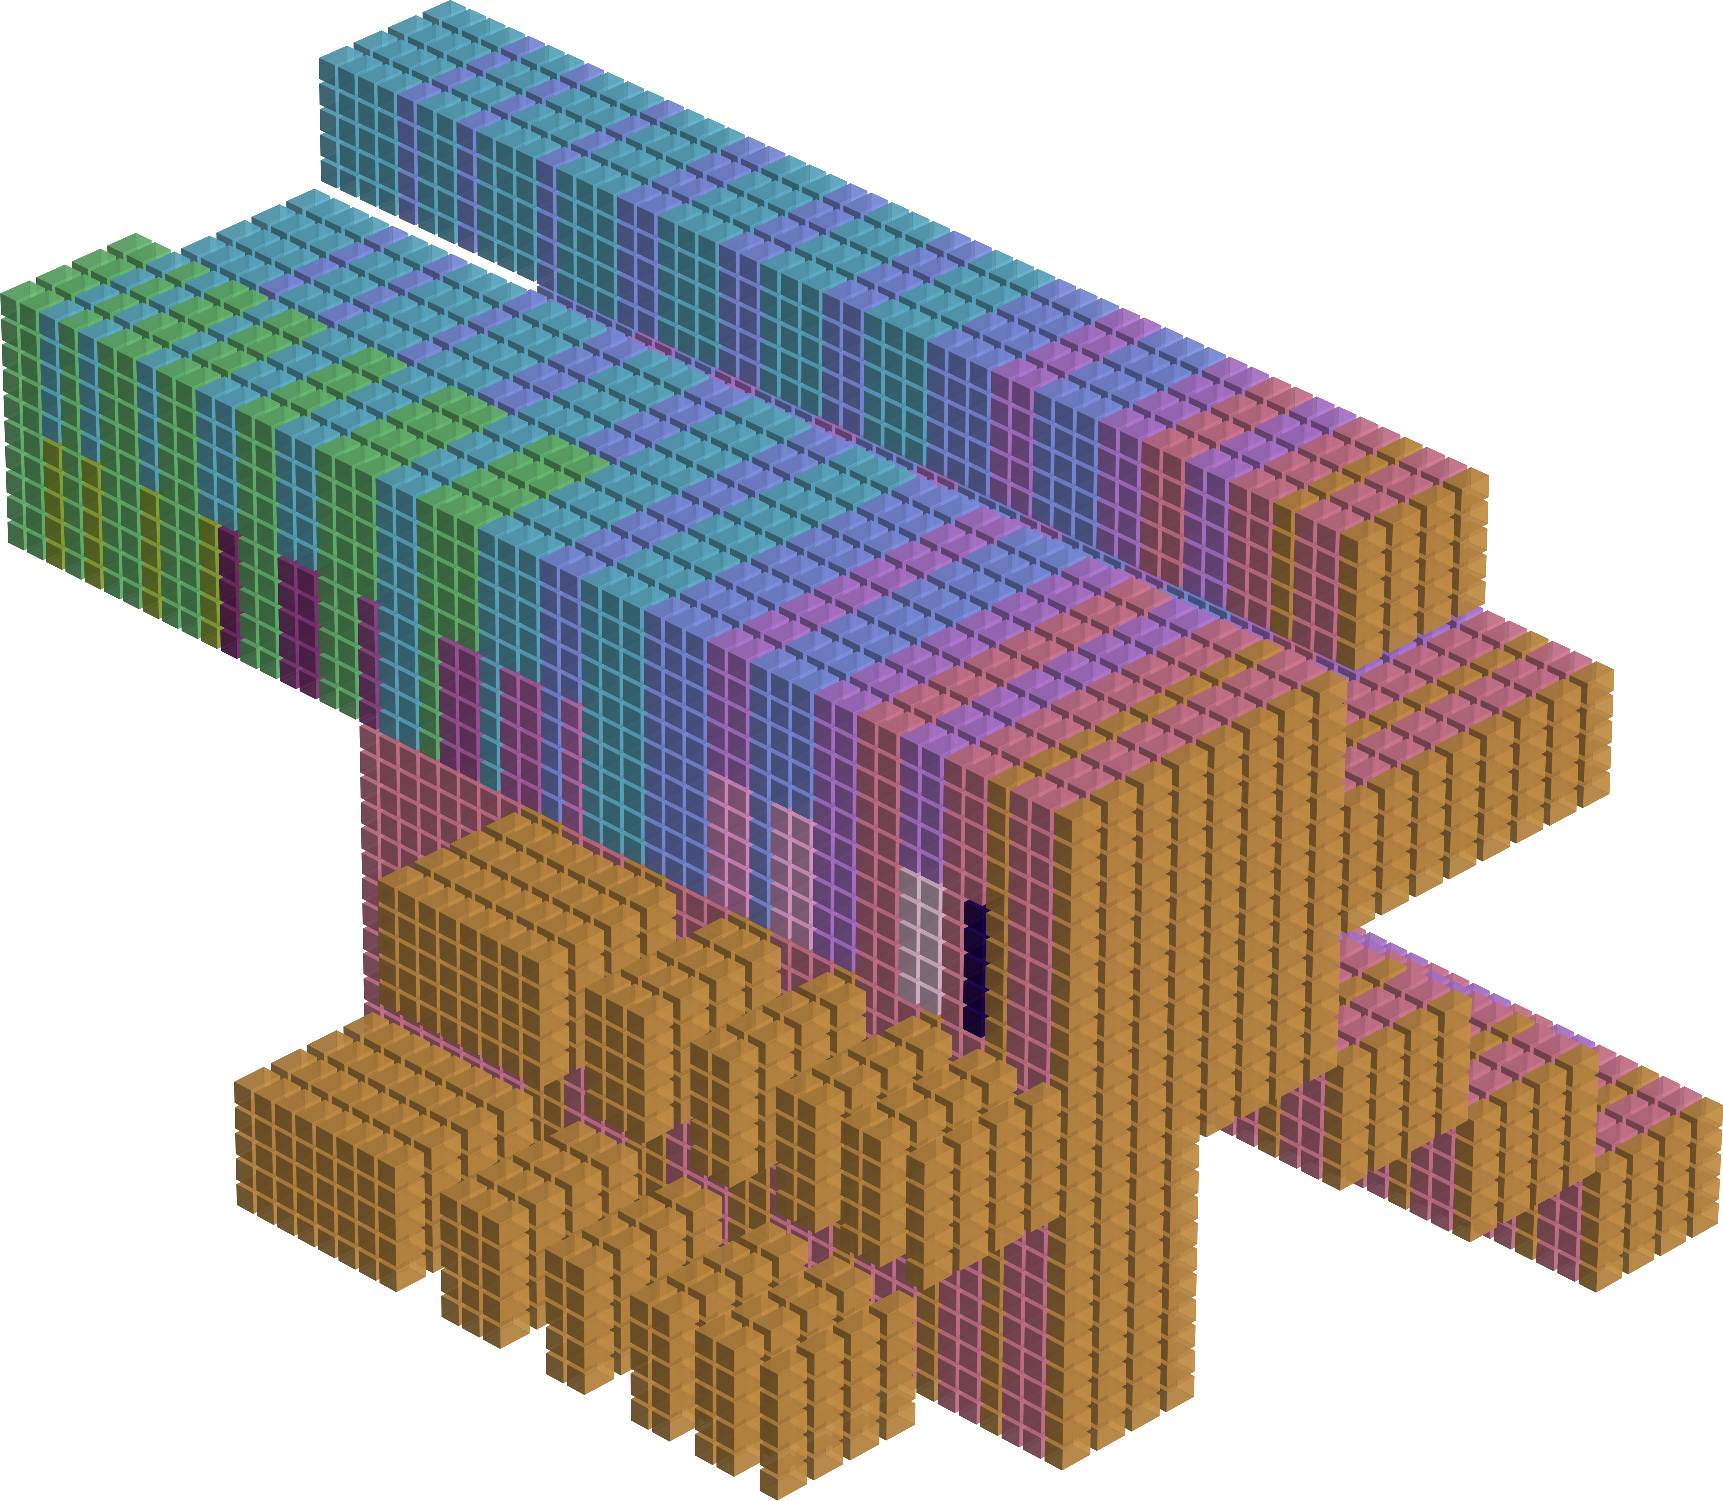
\includegraphics[width=10cm]{src/colorspace_patterns/pattern0-45.png}%
    \end{adjustbox}
    \begin{adjustbox}{width=10cm}
      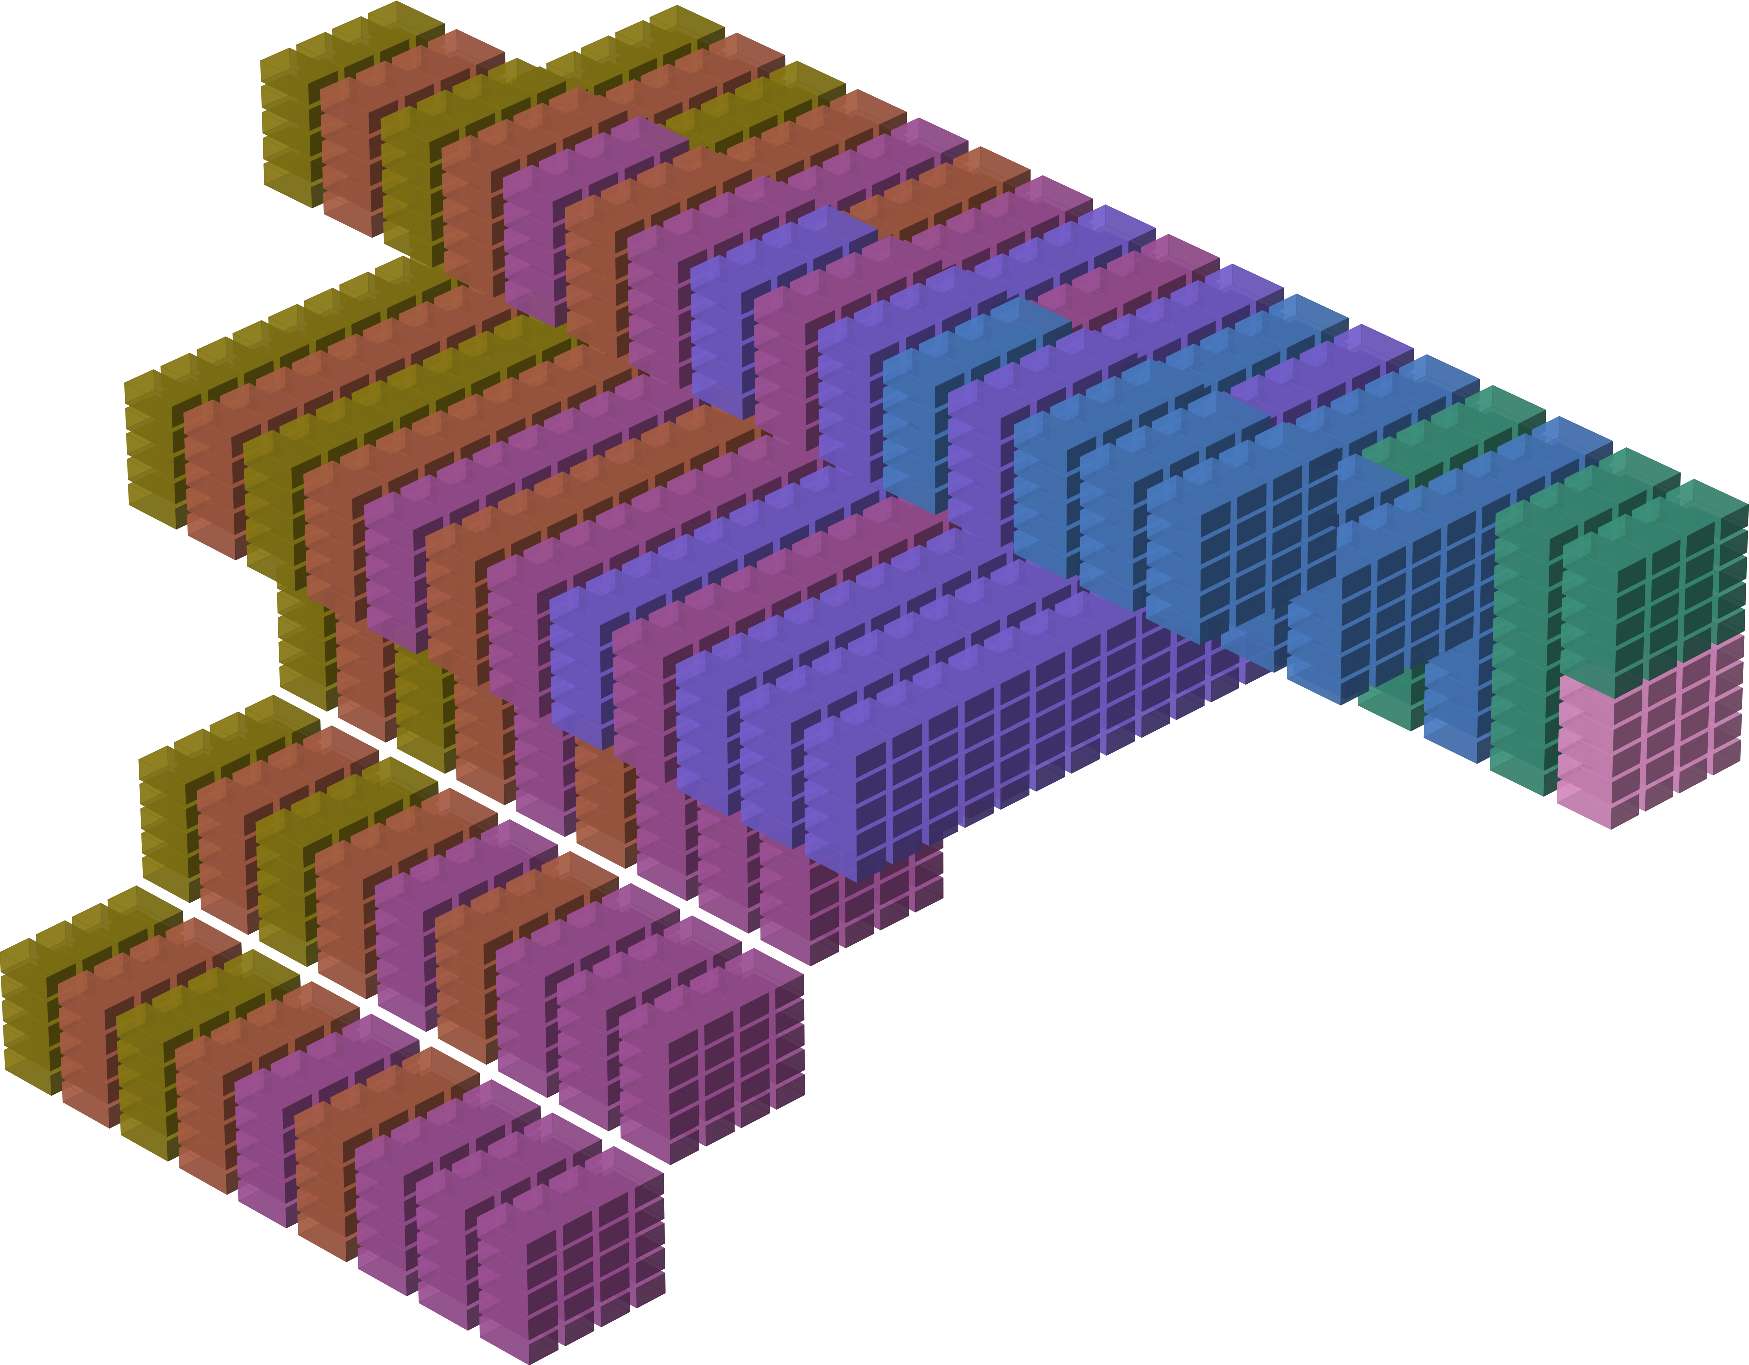
\includegraphics[width=10cm]{src/colorspace_patterns/pattern0-225.png}%
    \end{adjustbox}
\caption{Evolution of the 'Twist' pattern.}
\end{figure}
\clearpage

\rhead[]{The Twist}
\begin{lstlisting}[caption=Source code for the Twist]
theTwistXPosArray                        
        .BYTE $00,$55             ;     2  
        .BYTE $01,$02,$55         ;   12   
        .BYTE $01,$02,$03,$55     ;    333 
        .BYTE $01,$02,$03,$04,$55 ;  654   
        .BYTE $00,$00,$00,$55     ; 6 5 4  
        .BYTE $FF,$FE,$55         ;   5  4 
        .BYTE $55                 ;       4
theTwistYPosArray
        .BYTE $FF,$55
        .BYTE $FF,$FE,$55
        .BYTE $00,$00,$00,$55
        .BYTE $01,$02,$03,$04,$55
        .BYTE $01,$02,$03,$55
        .BYTE $01,$02,$55
        .BYTE $55
\end{lstlisting}

\subfile{colorspace_patterns/tables/pattern0.tex}


\clearpage
\textbf{Lines 1189-1231. \icode{\textbf{pixelXPositionLoPtrArray, pixelYPositionLoPtrArray}}} 
\begin{lstlisting}[basicstyle=\ttfamily\scriptsize,caption = All the pattern data structures in Colourspace organized into a set of arrays. 
We use these arrays to choose the correct user-selected pattern at painting time.]
; A pair of arrays together consituting a list of pointers
; to positions in memory containing X position data.
pixelXPositionLoPtrArray   
.BYTE <theTwistXPosArray,<smoothCrossflowXPosArray,<denturesXPosArray
.BYTE <deltoidsXPosArray,<pulsarCrossXPosArray,<slothMultiCrossXPosArray
.BYTE <crossAndABitXPosArray,<star2XPosArray,<userLightform0XPosArray
.BYTE <userLightform1XPosArray,<userLightform2XPosArray,<userLightform3XPosArray
.BYTE <userLightform4XPosArray,<userLightform5XPosArray,<userLightform6XPosArray
.BYTE <userLightform7XPosArray,<userLightform8XPosArray,<userLightform9XPosArray
.BYTE <userLightform10XPosArray,<userLightform11XPosArray,<userLightform12XPosArray
.BYTE <userLightform13XPosArray,<userLightform14XPosArray,<userLightform15XPosArray
.BYTE <a2800,<a2880,<a2900,<a2980,<a2A00,<a2A80,<a2B00,<a2B80

pixelXPositionHiPtrArray   
.BYTE >theTwistXPosArray,>smoothCrossflowXPosArray,>denturesXPosArray
.BYTE >deltoidsXPosArray,>pulsarCrossXPosArray,>slothMultiCrossXPosArray
.BYTE >crossAndABitXPosArray,>star2XPosArray,>userLightform0XPosArray
.BYTE >userLightform1XPosArray,>userLightform2XPosArray,>userLightform3XPosArray
.BYTE >userLightform4XPosArray,>userLightform5XPosArray,>userLightform6XPosArray
.BYTE >userLightform7XPosArray,>userLightform8XPosArray,>userLightform9XPosArray
.BYTE >userLightform10XPosArray,>userLightform11XPosArray,>userLightform12XPosArray
.BYTE >userLightform13XPosArray,>userLightform14XPosArray,>userLightform15XPosArray
.BYTE >a2800,>a2880,>a2900,>a2980,>a2A00,>a2A80,>a2B00,>a2B80

; A pair of arrays together consituting a list of pointers
; to positions in memory containing Y position data.
pixelYPositionLoPtrArray   
.BYTE <theTwistYPosArray,<smoothCrossflowYPosArray,<denturesYPosArray
.BYTE <deltoidsYPosArray,<pulsarCrossYPosArray,<slothMultiCrossYPosArray
.BYTE <crossAndABitYPosArray,<star2YPosArray,<userLightform0YPosArray
.BYTE <userLightform1YPosArray,<userLightform2YPosArray,<userLightform3YPosArray
.BYTE <userLightform4YPosArray,<userLightform5YPosArray,<userLightform6YPosArray
.BYTE <userLightform7YPosArray,<userLightform8YPosArray,<userLightform9YPosArray
.BYTE <userLightform10YPosArray,<userLightform11YPosArray,<userLightform12YPosArray
.BYTE <userLightform13YPosArray,<userLightform14YPosArray,<userLightform15YPosArray
.BYTE <a2840,<a28C0,<a2940,<a29C0,<a2A40,<a2AC0,<a2B40,<a2BC0

pixelYPositionHiPtrArray   
.BYTE >theTwistYPosArray,>smoothCrossflowYPosArray,>denturesYPosArray
.BYTE >deltoidsYPosArray,>pulsarCrossYPosArray,>slothMultiCrossYPosArray
.BYTE >crossAndABitYPosArray,>star2YPosArray,>userLightform0YPosArray
.BYTE >userLightform1YPosArray,>userLightform2YPosArray,>userLightform3YPosArray
.BYTE >userLightform4YPosArray,>userLightform5YPosArray,>userLightform6YPosArray
.BYTE >userLightform7YPosArray,>userLightform8YPosArray,>userLightform9YPosArray
.BYTE >userLightform10YPosArray,>userLightform11YPosArray,>userLightform12YPosArray
.BYTE >userLightform13YPosArray,>userLightform14YPosArray,>userLightform15YPosArray
.BYTE >a2840,>a28C0,>a2940,>a29C0,>a2A40,>a2AC0,>a2B40,>a2BC0
\end{lstlisting}
\clearpage

\rhead[]{\icode{pixelXPositionLoPtrArray/pixelXPositionHiPtrArray}}
\textbf{Lines 1189-1231. \icode{\textbf{pixelXPositionLoPtrArray/pixelXPositionHiPtrArray}}:} Psychedelia
offers 16 different pretty patterns to choose from, so requires some way of managing them, particularly
when it comes time to painting them on the screen. The four arrays on the opposite page do this job.
They allow us to reference each pattern with an index. For example, index 0 will reference the X and
Y Position data structures for the 'Star One' pattern in \icode{starOneXPosArray} and 
\icode{starOneYPosArray}, index 1 will allow us to reference the data structures for 'The Twist' pattern,
and so on.

On the following pages we'll see how we make practical use of these arrays, but for now we only really
need to make clear that each one contains one byte of the two-byte address at which each
data structure is stored. The use of \icode{<} and \icode{>} in the listing is a convention that
tells the assembler we're looking at the first byte (\icode{>}) or the second byte (\icode{<}).
Hopefully this table makes this explicit to the reader:

\begin{figure}[H]
  {
    \setlength{\tabcolsep}{3.0pt}
    \setlength\cmidrulewidth{\heavyrulewidth} % Make cmidrule = 
    \begin{adjustbox}{width=8cm,center}
      \begin{tabular}{ccccc}
        \toprule
        Element &
        \makecell[c]{\icode{pixelXPosition} \\ \icode{HiPtrArray}} & 
        \makecell[c]{\icode{pixelXPosition} \\ \icode{LoPtrArray}} & 
        Address &
        Name \\
        \midrule
        0 & \icode{\$09} & \icode{\$7C} & \icode{\$097C} & \icode{starOneXPosArray} \\ 
        1 & \icode{\$0E} & \icode{\$93} & \icode{\$0E93}  & \icode{theTwistXPosArray}\\ 
        2 & \icode{\$0E} & \icode{\$C3} & \icode{\$0EC3}  & \icode{laLlamitaXPosArray}\\ 
        3 & \icode{\$0F} & \icode{\$07} & \icode{\$0F07}  & \icode{starTwoXPosArray}\\ 
        4 & \icode{\$0F} & \icode{\$23} & \icode{\$0F23}  & \icode{deltoidXPosArray}\\ 
        5 & \icode{\$0F} & \icode{\$57} & \icode{\$0F57}  & \icode{diffusedXPosArray}\\ 
        . & . & . & . &. \\
        15 & \icode{\$CE} & \icode{\$00} & \icode{\$CE00}  & \icode{customPattern6XPosArray}\\ 
        16 & \icode{\$CF} & \icode{\$00} & \icode{\$CF00}  & \icode{customPattern7XPosArray}\\ 
        \bottomrule
      \end{tabular}
    \end{adjustbox}
  }\caption{Our two arrays and their contents - each combining to give us an address for the X
  Position data structure for each pattern. The line with ellipses indicates that we've left out some elements for the
  sake of brevity.}
\end{figure}
\vspace*{-\baselineskip}

\textbf{Lines 1189-1231. \icode{\textbf{pixelYPositionLoPtrArray/pixelYPositionHiPtrArray}}:} As for the X position array,
so for the Y position array. 
\begin{figure}[H]
  {
    \setlength{\tabcolsep}{3.0pt}
    \setlength\cmidrulewidth{\heavyrulewidth} % Make cmidrule = 
    \begin{adjustbox}{width=8cm,center}
      \begin{tabular}{ccccc}
        \toprule
        Element &
        \makecell[c]{\icode{pixelYPosition} \\ \icode{HiPtrArray}} & 
        \makecell[c]{\icode{pixelYPosition} \\ \icode{LoPtrArray}} & 
        Address &
        Name \\
        \midrule
        0 & \icode{\$09} & \icode{\$A3} & \icode{\$09A3} & \icode{starOneYPosArray} \\ 
        1 & \icode{\$0E} & \icode{\$AB} & \icode{\$0EAB}  & \icode{theTwistYPosArray}\\ 
        2 & \icode{\$0E} & \icode{\$E5} & \icode{\$0EE5}  & \icode{laLlamitaYPosArray}\\ 
        . & . & . & . &. \\
        15 & \icode{\$CE} & \icode{\$00} & \icode{\$CE00}  & \icode{customPattern6YPosArray}\\ 
        16 & \icode{\$CF} & \icode{\$00} & \icode{\$CF00}  & \icode{customPattern7YPosArray}\\ 
        \bottomrule
      \end{tabular}
    \end{adjustbox}
  }\caption{Our two arrays and their contents - each combining to give us an address for the Y
  Position data structure for each pattern. }
\end{figure}

%
\begin{minipage}[b]{0.48\linewidth}
\begin{figure}[H]
    \centering
    \begin{adjustbox}{width=5cm,margin=0cm 0cm}
      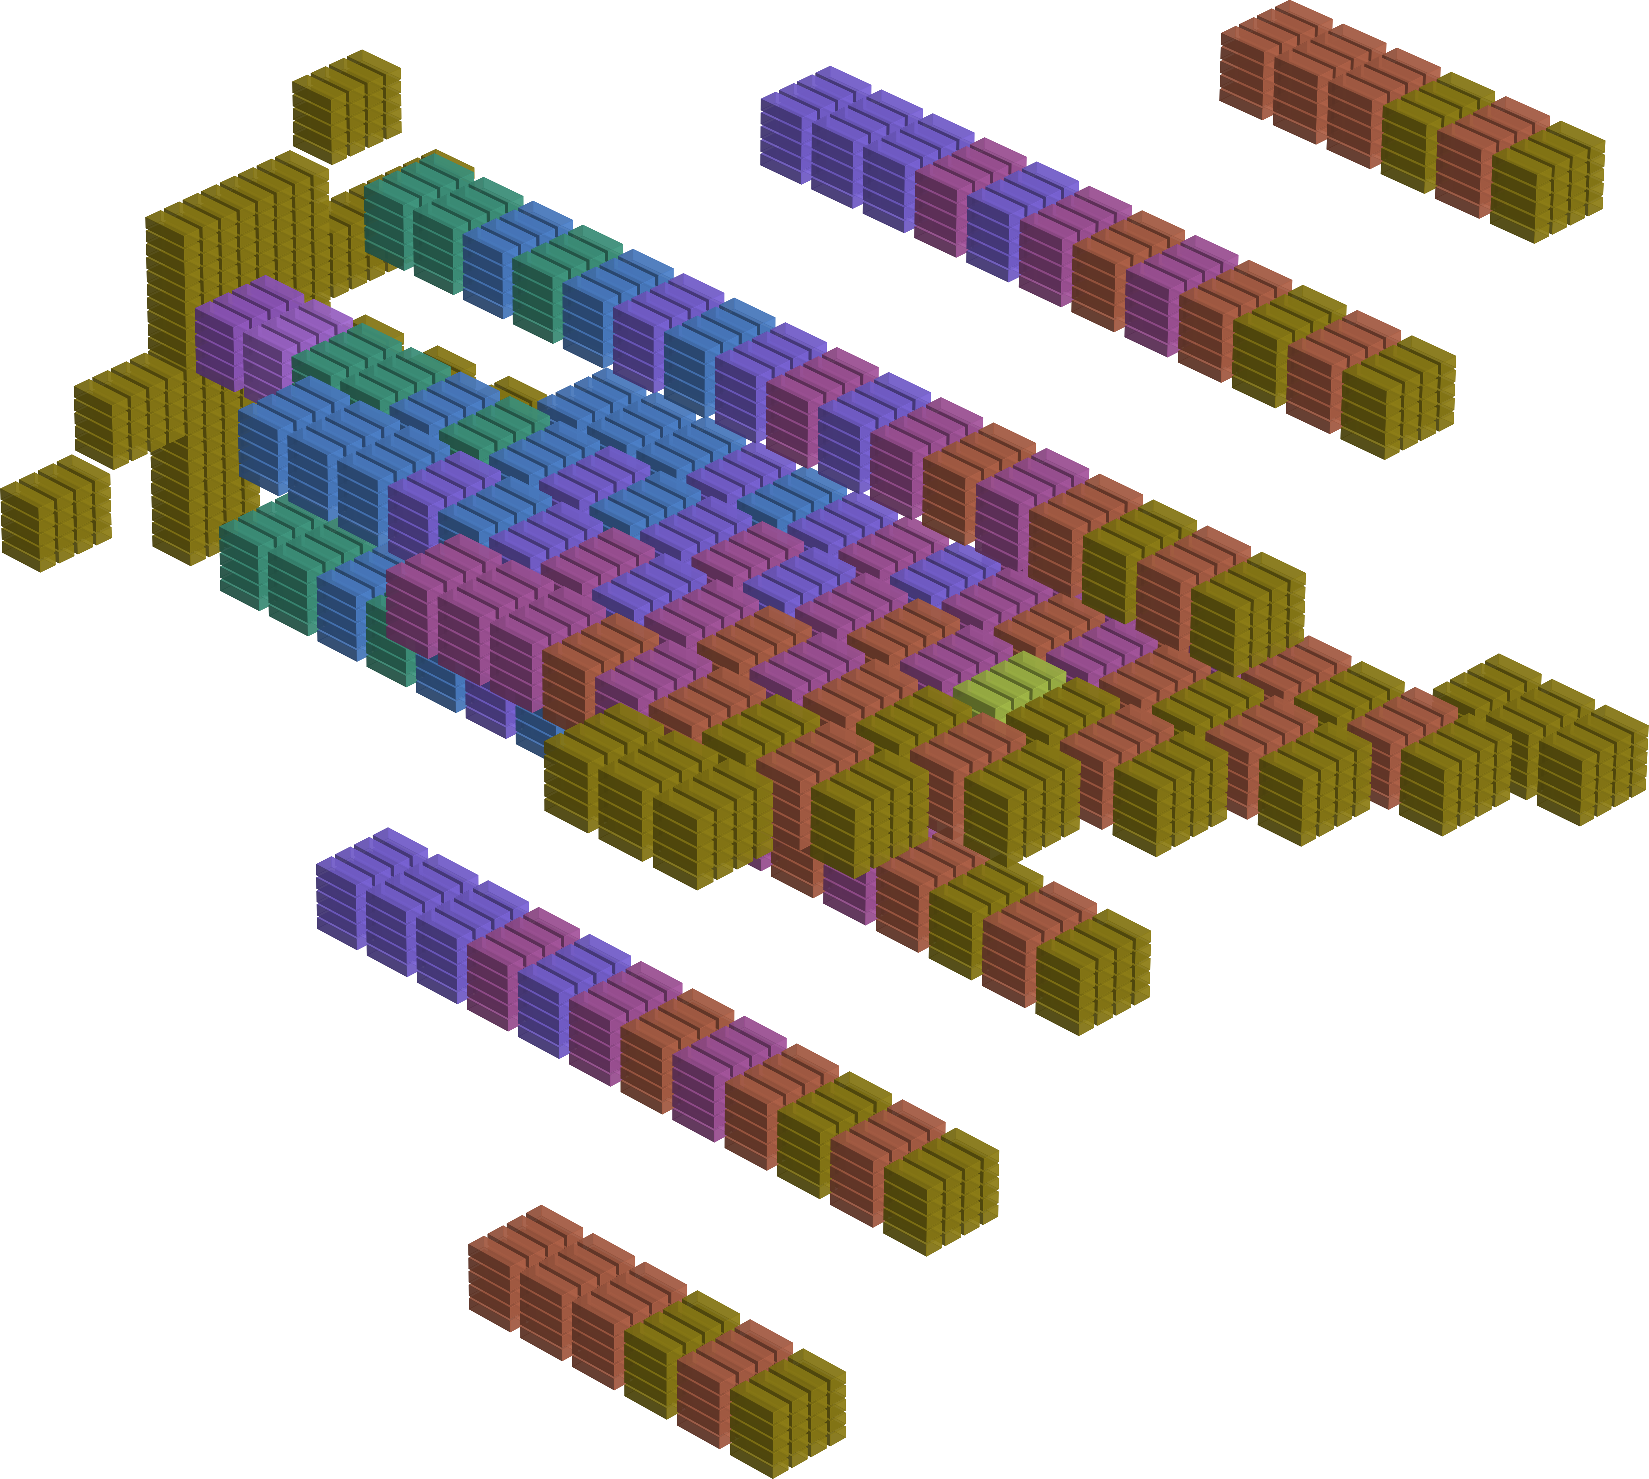
\includegraphics[width=10cm]{src/colorspace_patterns/pattern1-45.png}%
    \end{adjustbox}
    \begin{adjustbox}{width=5cm,margin=0cm 0cm}
      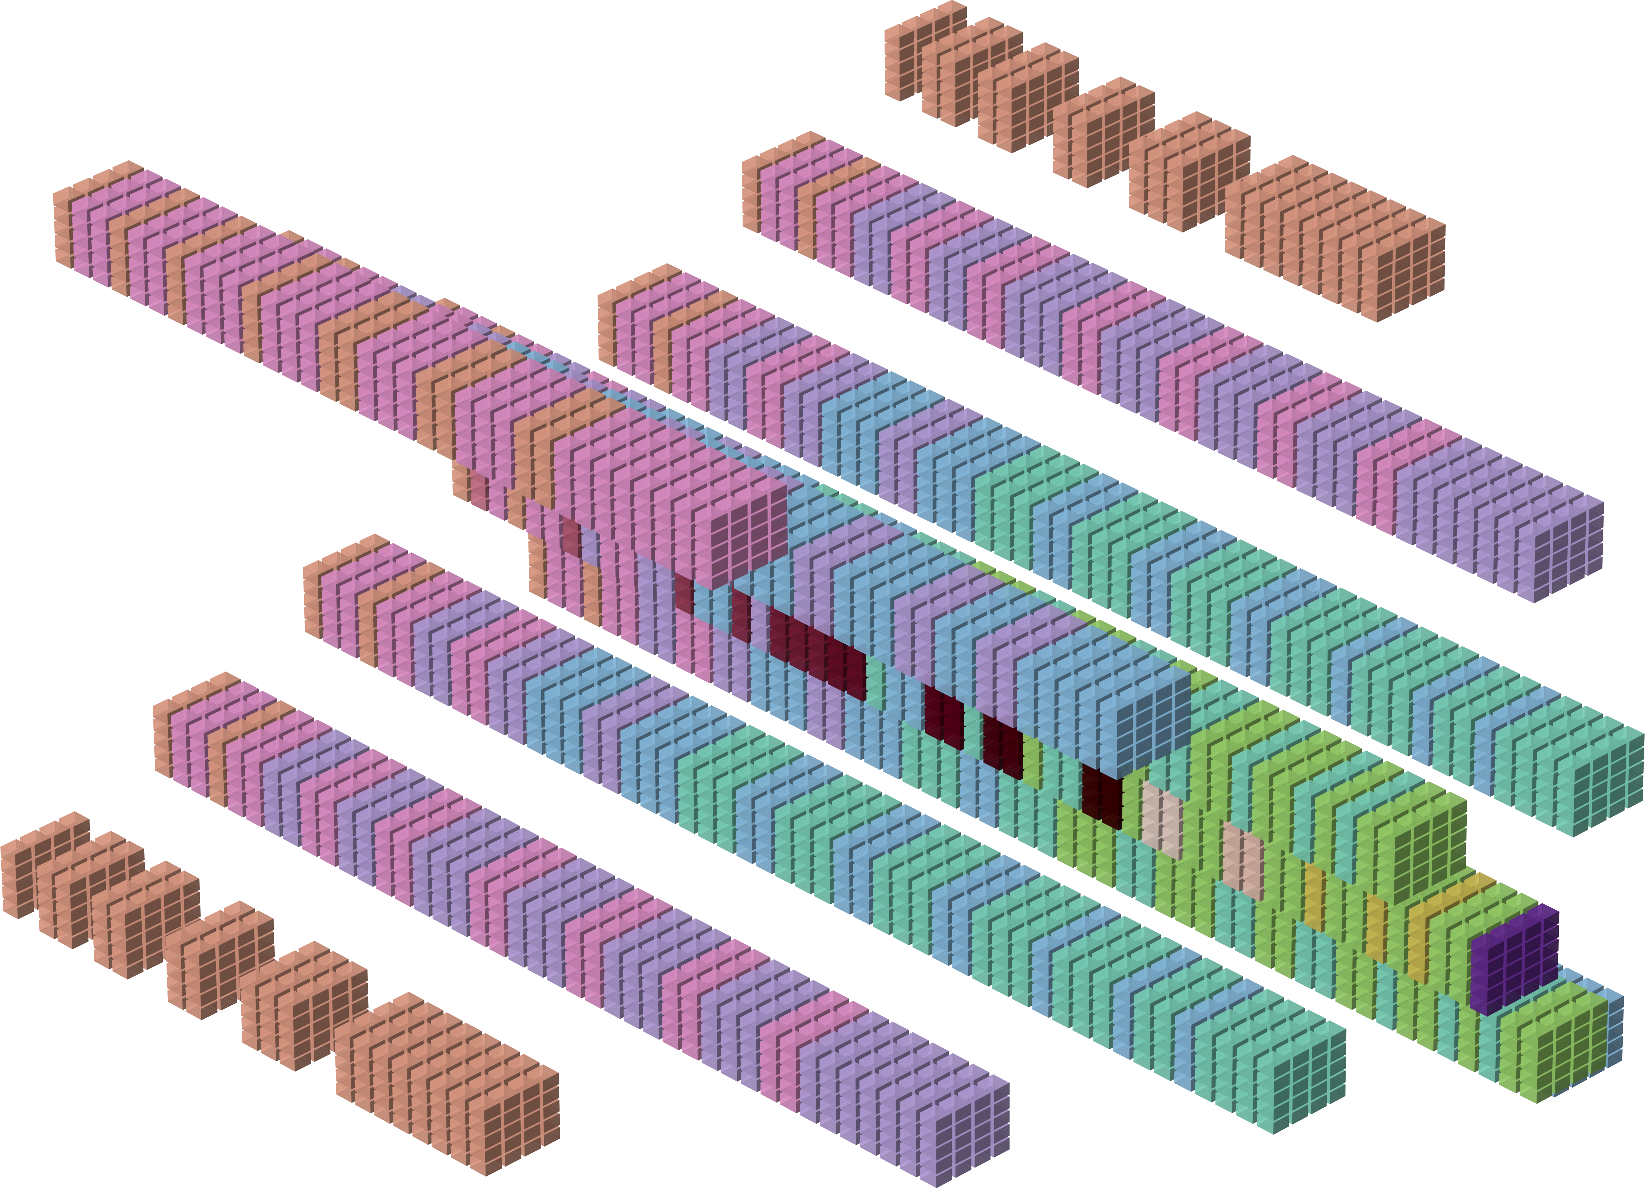
\includegraphics[width=10cm]{src/colorspace_patterns/pattern1-225.png}%
    \end{adjustbox}
\caption{The 'Smooth Crossflow'.}
\end{figure}
\end{minipage}
\begin{minipage}[b]{0.48\linewidth}
\begin{lrbox}{\mybox}%
\begin{lstlisting}[basicstyle=\ttfamily\tiny,escapechar=\%]
smoothCrossflowXPosArray
        .BYTE $FF,$01,$55        ;            5
        .BYTE $FE,$02,$55        ;              
        .BYTE $FD,$03,$55        ;          3   
        .BYTE $FC,$04,$55        ; 6            
        .BYTE $FB,$05,$55        ;   4    1     
        .BYTE $FA,$06,$55        ;     2        
        .BYTE $55                ;              
smoothCrossflowYPosArray         ;         2    
        .BYTE $02,$FE,$55        ;      1    4  
        .BYTE $FF,$01,$55        ;             6
        .BYTE $04,$FC,$55        ;    3         
        .BYTE $FE,$02,$55        ;              
        .BYTE $06,$FA,$55        ;  5           
        .BYTE $FD,$03,$55
        .BYTE $55
\end{lstlisting}
\end{lrbox}%
\scalebox{0.8}{\usebox{\mybox}}
\subfile{colorspace_patterns/tables/pattern1.tex}
\end{minipage}
%
%
\begin{minipage}[b]{0.48\linewidth}
\vspace{1cm}
\begin{figure}[H]
    \centering
    \begin{adjustbox}{width=5cm,margin=0cm 0cm}
      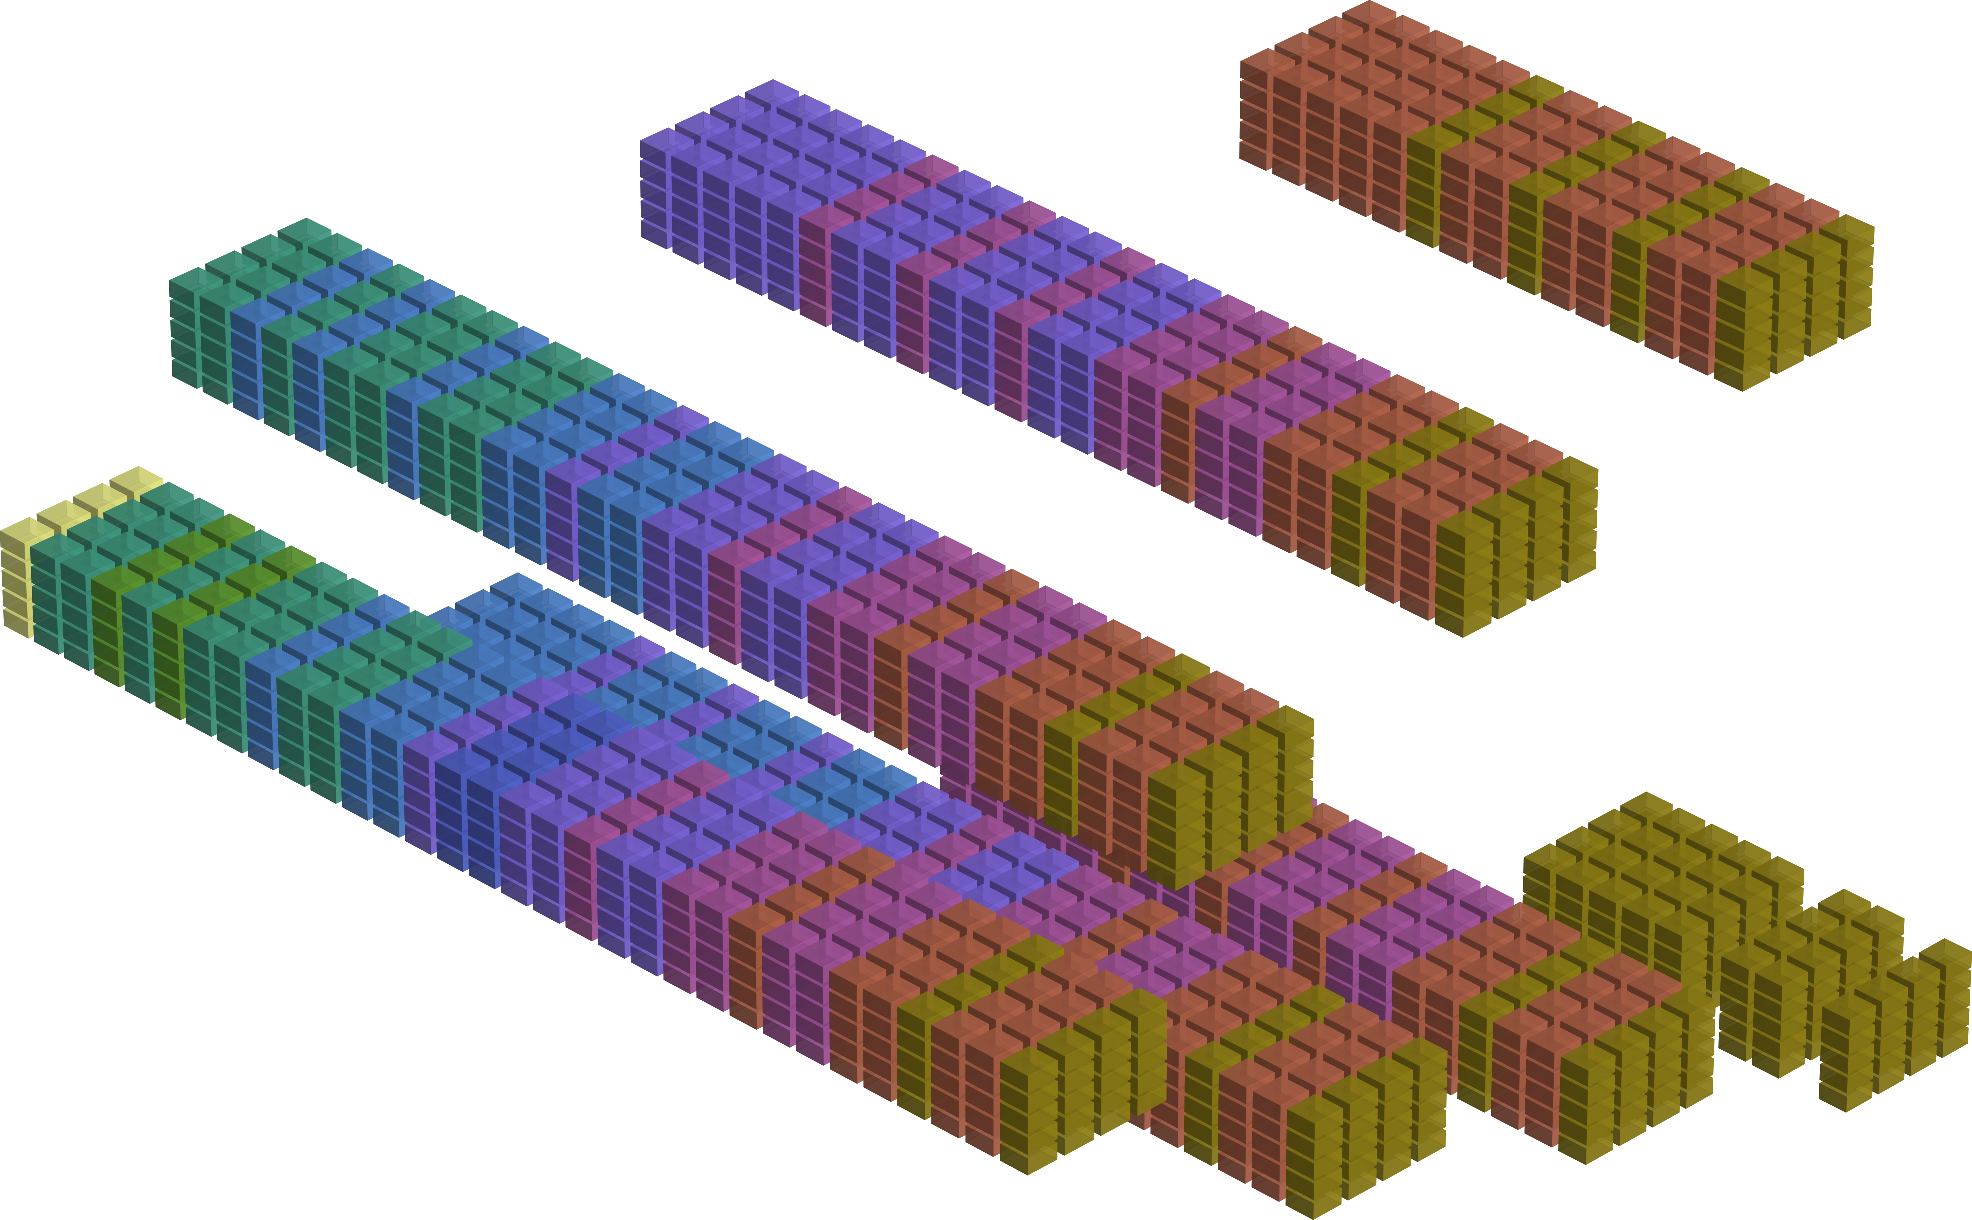
\includegraphics[width=10cm]{src/colorspace_patterns/pattern2-45.png}%
    \end{adjustbox}
    \begin{adjustbox}{width=5cm,margin=0cm 0cm}
      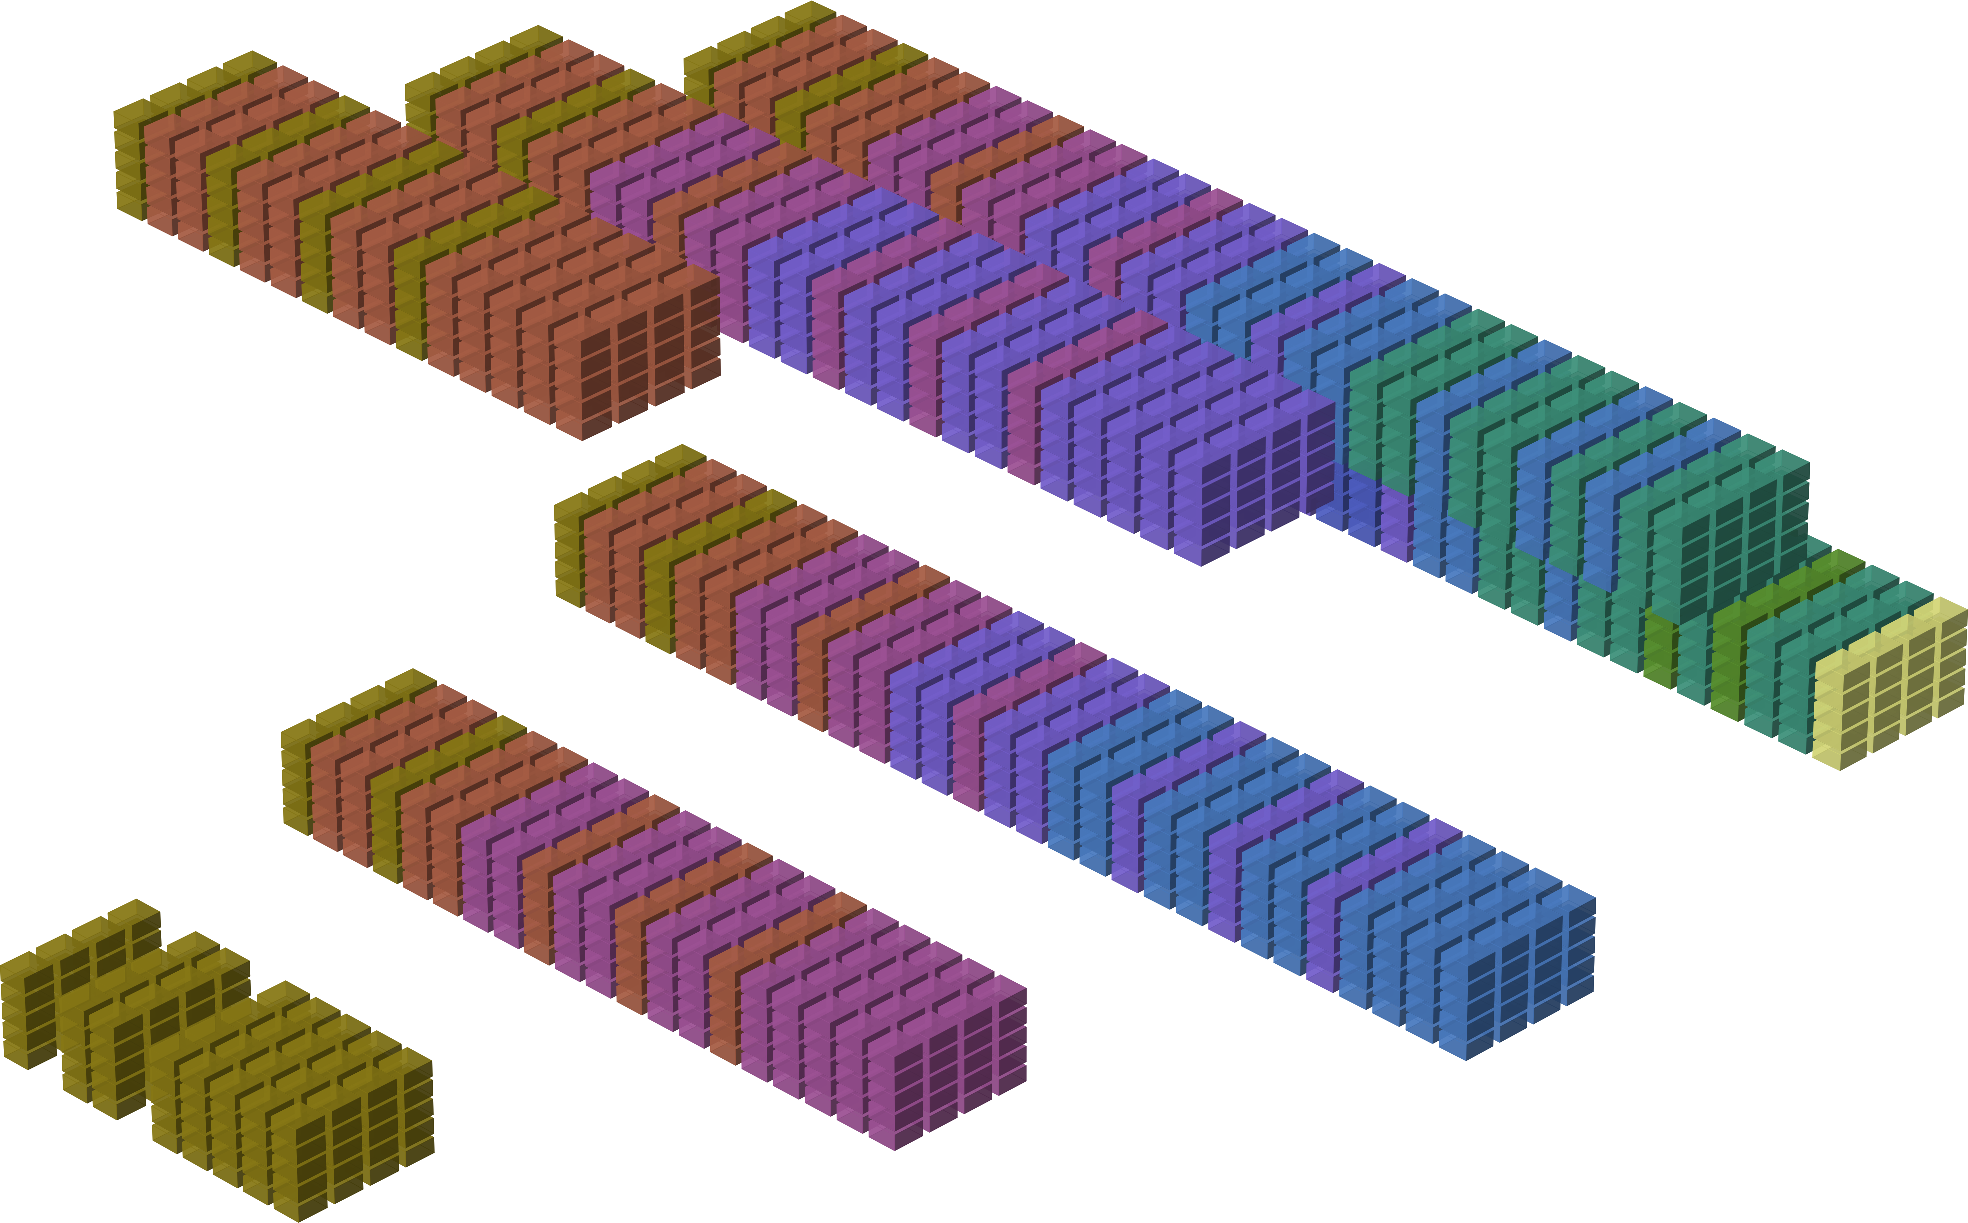
\includegraphics[width=10cm]{src/colorspace_patterns/pattern2-225.png}%
    \end{adjustbox}
\caption{'The Dentures'.}
\end{figure}
\end{minipage}
\begin{minipage}[b]{0.48\linewidth}
\vspace{1cm}
\begin{lrbox}{\mybox}%
\begin{lstlisting}[basicstyle=\ttfamily\tiny,escapechar=\%]
denturesXPosArray
        .BYTE $01,$55            ;      5 
        .BYTE $02,$55            ;    3   
        .BYTE $03,$55            ;  1     
        .BYTE $04,$55            ;        
        .BYTE $05,$55            ;        
        .BYTE $06,$55            ;        
        .BYTE $55                ;   2    
denturesYPosArray                ;     4  
        .BYTE $FE,$55            ;       6
        .BYTE $02,$55
        .BYTE $FD,$55
        .BYTE $03,$55
        .BYTE $FC,$55
        .BYTE $04,$55
        .BYTE $55
\end{lstlisting}
\end{lrbox}%
\scalebox{0.8}{\usebox{\mybox}}
\subfile{colorspace_patterns/tables/pattern2.tex}
\end{minipage}
%
%
\begin{minipage}[b]{0.48\linewidth}
\begin{figure}[H]
    \centering
    \begin{adjustbox}{width=5cm,margin=0cm 0cm}
      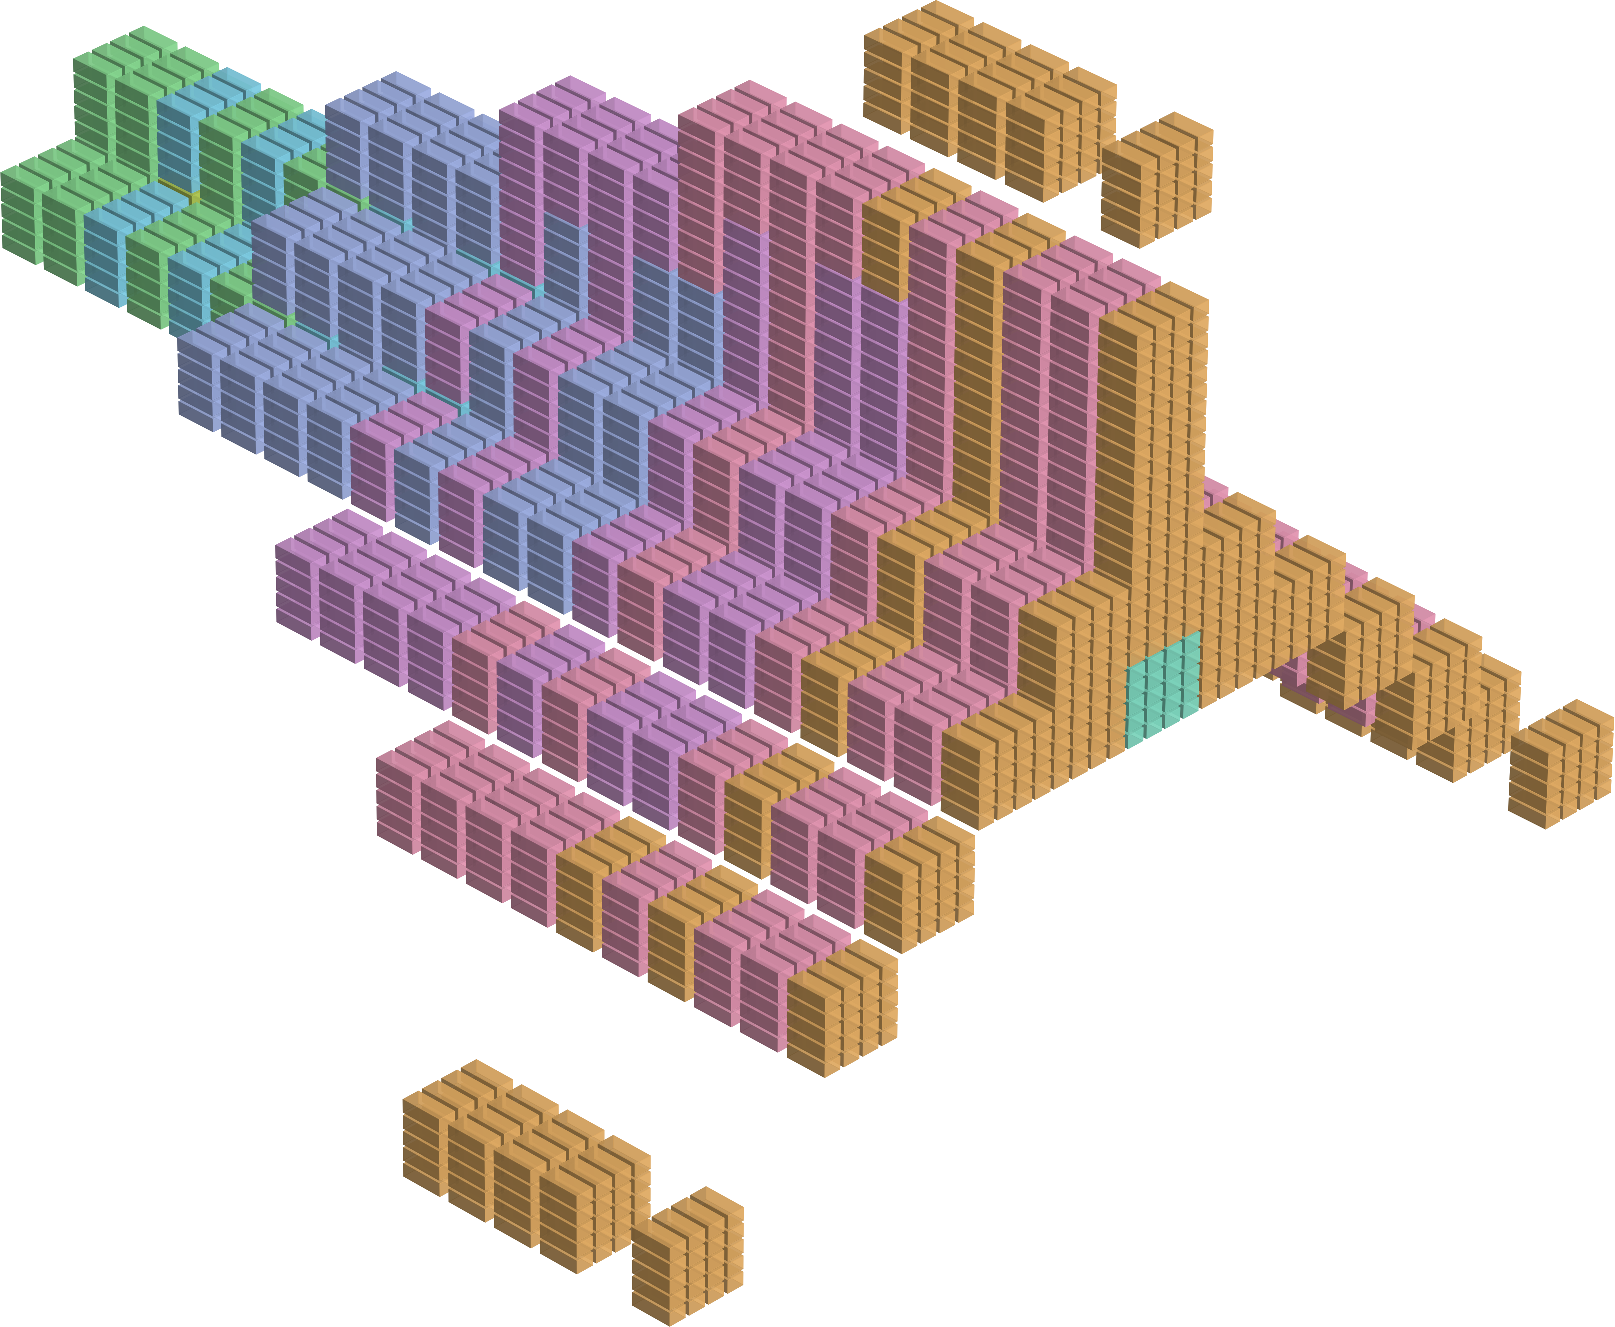
\includegraphics[width=10cm]{src/colorspace_patterns/pattern3-45.png}%
    \end{adjustbox}
    \begin{adjustbox}{width=5cm,margin=0cm 0cm}
      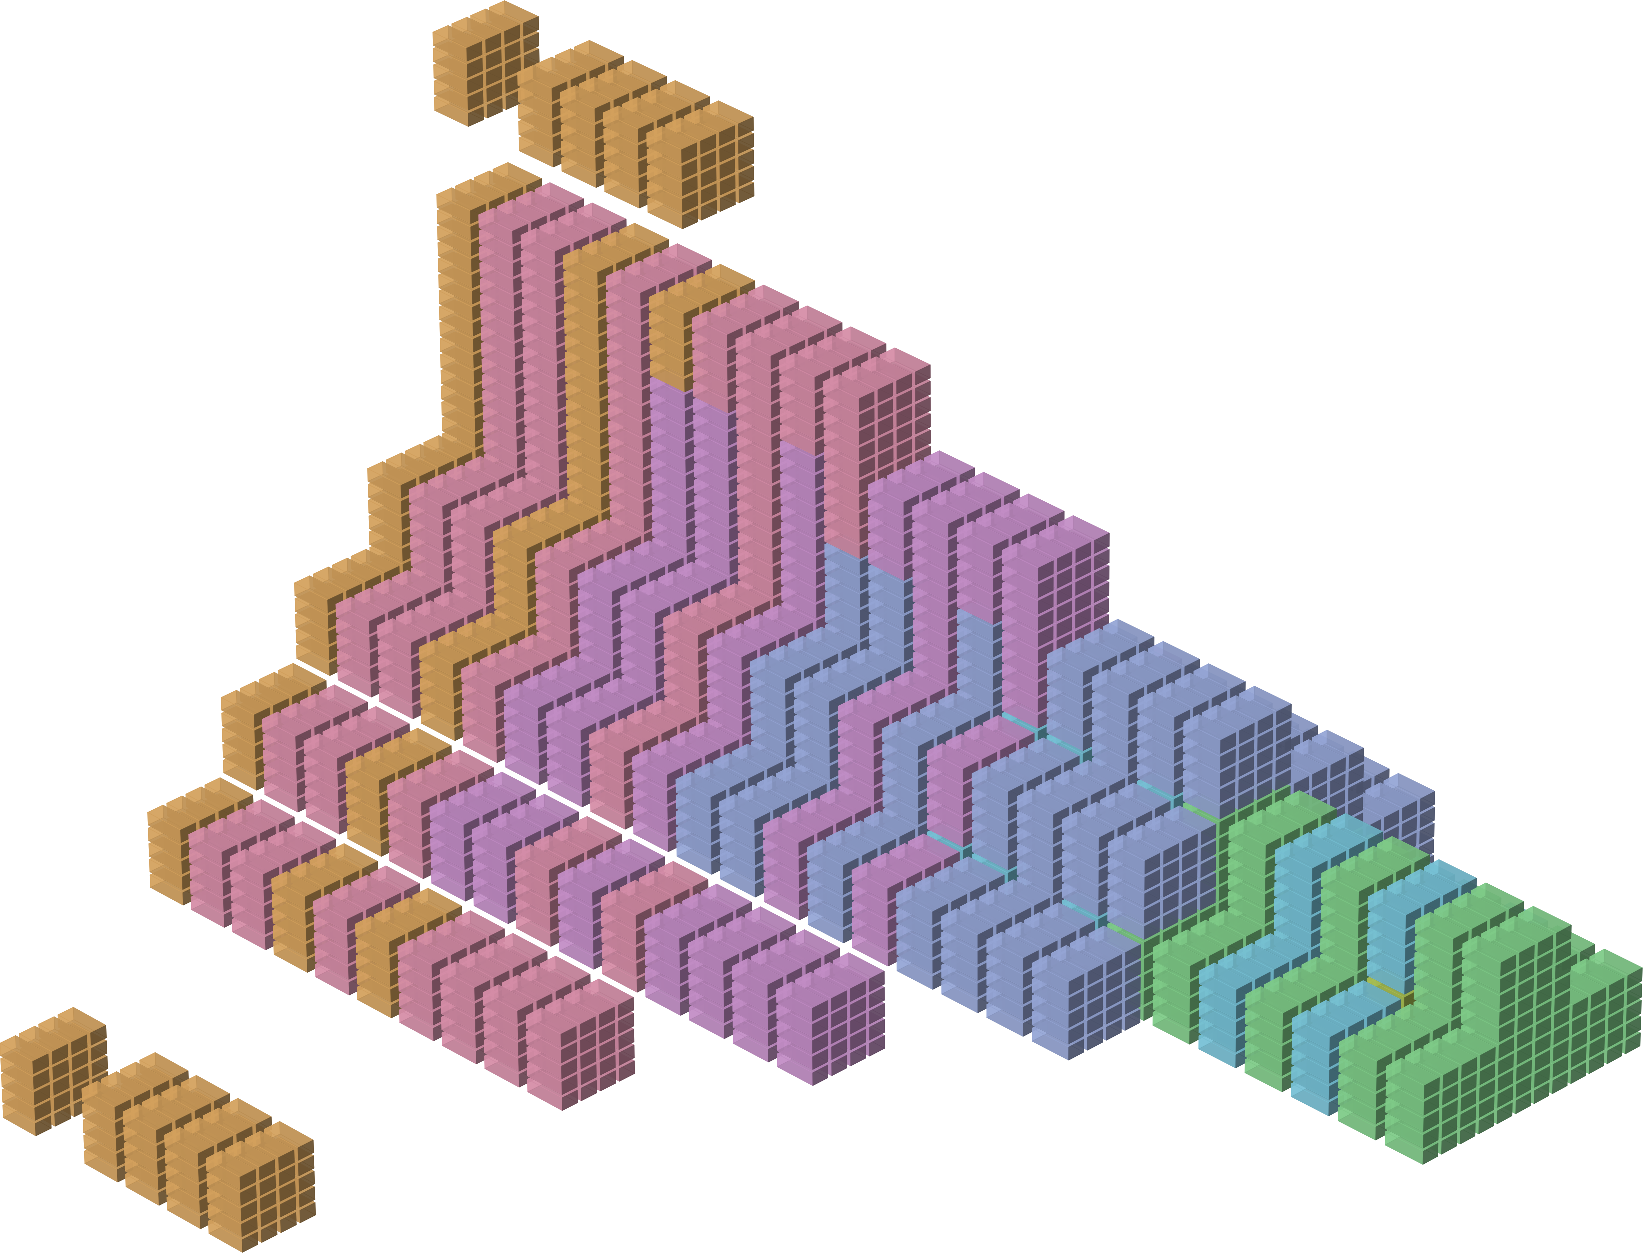
\includegraphics[width=10cm]{src/colorspace_patterns/pattern3-225.png}%
    \end{adjustbox}
\caption{'Deltoids'.}
\end{figure}
\end{minipage}
\begin{minipage}[b]{0.48\linewidth}
\begin{lrbox}{\mybox}%
\hspace{1cm}
\begin{lstlisting}[basicstyle=\ttfamily\tiny,escapechar=\%]
deltoidsXPosArray                     
        .BYTE $FF,$00,$01,$55         ;       6      
        .BYTE $55                     ;              
        .BYTE $FE,$FF,$00,$01,$02,$55 ;       5      
        .BYTE $FD,$00,$03,$55         ;       4      
        .BYTE $FC,$00,$04,$55         ;       3      
        .BYTE $FA,$00,$06,$55         ;      313     
        .BYTE $55                     ;     31 13    
deltoidsYPosArray                     ;    4     4   
        .BYTE $00,$FF,$00,$55         ;   5       5  
        .BYTE $55                     ;              
        .BYTE $00,$FF,$FE,$FF,$00,$55 ; 6           6
        .BYTE $01,$FD,$01,$55
        .BYTE $02,$FC,$02,$55
        .BYTE $04,$FA,$04,$55
        .BYTE $55
\end{lstlisting}
\end{lrbox}%
\scalebox{0.8}{\usebox{\mybox}}
\subfile{colorspace_patterns/tables/pattern3.tex}
\end{minipage}
%
%
\begin{minipage}[b]{0.48\linewidth}
\vspace{0.5cm}
\begin{figure}[H]
    \centering
    \begin{adjustbox}{width=6cm,margin=0.5cm 0cm}
      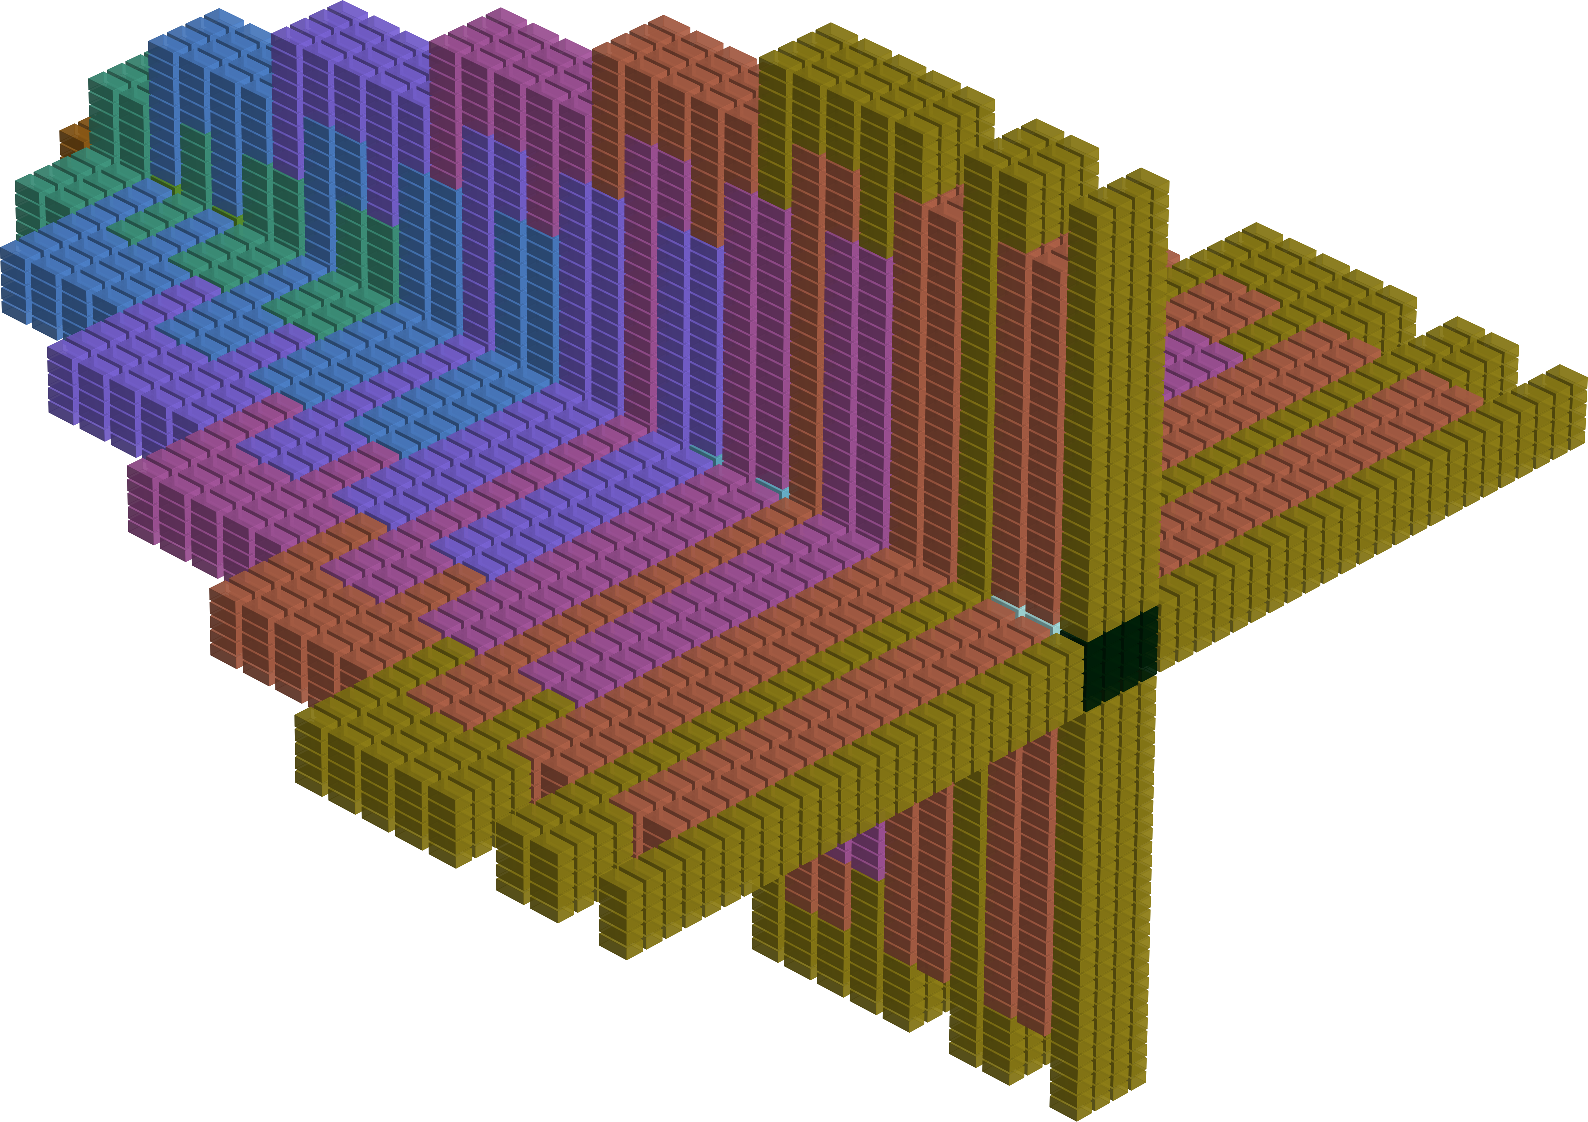
\includegraphics[width=10cm]{src/colorspace_patterns/pattern4-45.png}%
    \end{adjustbox}
    \begin{adjustbox}{width=6cm,margin=0cm 0cm}
      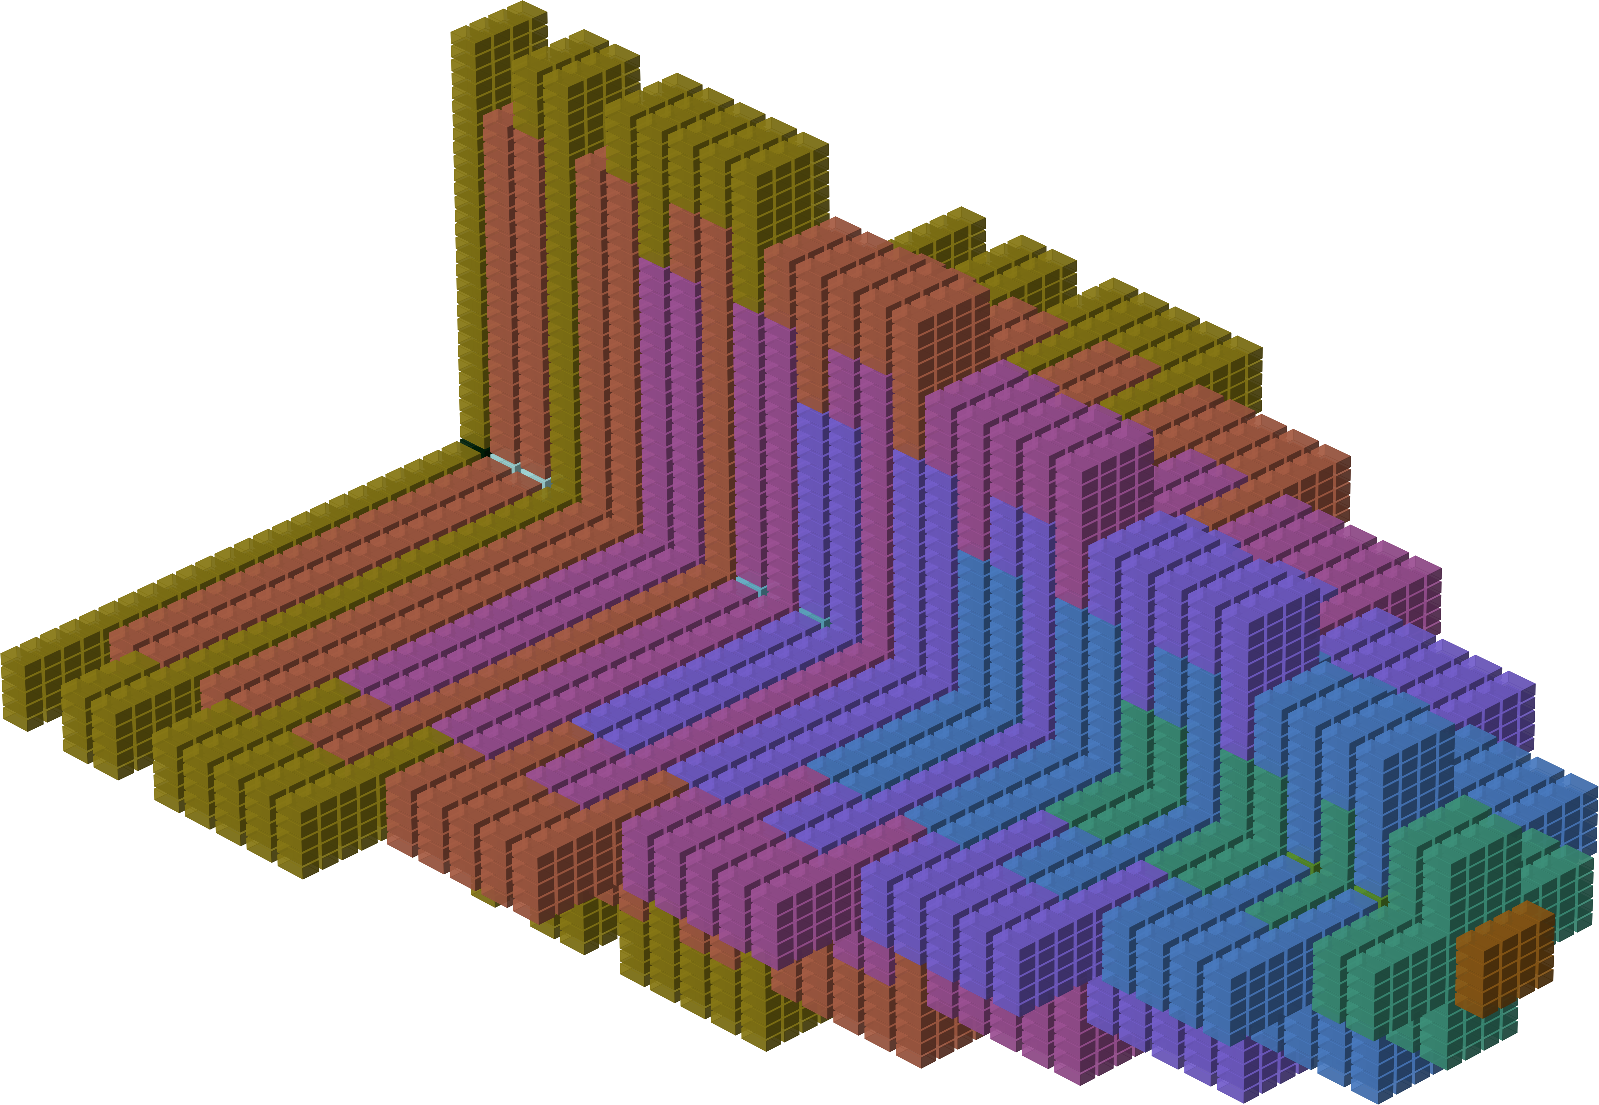
\includegraphics[width=10cm]{src/colorspace_patterns/pattern4-225.png}%
    \end{adjustbox}
\caption{'Pulsar Cross'.}
\end{figure}
\end{minipage}
\begin{minipage}[b]{0.48\linewidth}
\vspace{0.5cm}
\begin{lrbox}{\mybox}%
\hspace{1.5cm}
\begin{lstlisting}[basicstyle=\ttfamily\tiny,escapechar=\%]
pulsarCrossXPosArray
.BYTE $00,$01,$00,$FF,$55     ;       6      
.BYTE $00,$02,$00,$FE,$55     ;       5      
.BYTE $00,$03,$00,$FD,$55     ;       4      
.BYTE $00,$04,$00,$FC,$55     ;       3      
.BYTE $00,$05,$00,$FB,$55     ;       2      
.BYTE $00,$06,$00,$FA,$55     ;       1      
.BYTE $55                     ; 654321 123456
pulsarCrossYPosArray          ;       1      
.BYTE $FF,$00,$01,$00,$55     ;       2      
.BYTE $FE,$00,$02,$00,$55     ;       3      
.BYTE $FD,$00,$03,$00,$55     ;       4      
.BYTE $FC,$00,$04,$00,$55     ;       5      
.BYTE $FB,$00,$05,$00,$55     ;       6      
.BYTE $FA,$00,$06,$00,$55
.BYTE $55
\end{lstlisting}
\end{lrbox}%
\scalebox{0.8}{\usebox{\mybox}}
\subfile{colorspace_patterns/tables/pattern4.tex}
\end{minipage}
\clearpage
\textbf{Lines 1189-1231. \icode{\textbf{PaintStructureAtCurrentPosition}}} 
\begin{lstlisting}[basicstyle=\ttfamily\scriptsize, caption=The routine responsible for painting patterns.]
PaintStructureAtCurrentPosition
        LDA currentPixelXPosition
        STA previousPixelXPosition
        LDA currentPixelYPosition
        STA previousPixelYPosition
        LDA currentPaintState
        AND #$80
        BEQ DoANormalPaint
        JMP PaintExplosionMode

DoANormalPaint   
        JSR PaintPixelForCurrentSymmetry
        LDA pixelsToPaint
        CMP #NUM_ARRAYS
        BNE HasPixelsToPaint
        RTS 

HasPixelsToPaint   
        LDX patternIndex
        LDA pixelXPositionLoPtrArray,X
        STA xPosLoPtr
        LDA pixelXPositionHiPtrArray,X
        STA xPosHiPtr
        LDA pixelYPositionLoPtrArray,X
        STA yPosLoPtr
        LDA pixelYPositionHiPtrArray,X
        STA yPosHiPtr

        LDA #NUM_ARRAYS
        STA countToMatchCurrentIndex
        LDY #$00
PixelPaintLoop
        LDA (xPosLoPtr),Y
        CMP #$55
        BEQ ReachedEndOfLine
        CLC 
        ADC currentPixelXPosition
        STA previousPixelXPosition
        LDA (yPosLoPtr),Y
        CLC 
        ADC currentPixelYPosition
        STA previousPixelYPosition
        TYA 
        PHA 
        JSR PaintPixelForCurrentSymmetry
        PLA 
        TAY 
        INY 
        JMP PixelPaintLoop

ReachedEndOfLine   
        DEC countToMatchCurrentIndex
        INY 
        LDA pixelsToPaint
        CMP countToMatchCurrentIndex
        BNE PixelPaintLoop
        STA ATRACT   ;ATRACT  screen attract counter
        RTS 
\end{lstlisting}
\clearpage

\rhead[]{\icode{PaintStructureAtCurrentPosition}}
\textbf{Lines 1189-1231. \icode{\textbf{PaintStructureAtCurrentPosition}}:} We've already encountered this routine
in \hyperref[sec:listing_commentary]{\textcolor{blue}{ our walk through of the listing.}}. This is the version that shipped 
with the commercial edition of Psychedelia so has a necessary extra complication to deal with the fact that we 
are going to paint one of up to 16 possible patterns. What we want to figure out here is the X and Y position we should
paint for each element in the pattern's data structure.

The pattern the user has selected is stored as an index value in \icode{patternIndex}. We use it to fetch the element
from each array:
\begin{lstlisting}[basicstyle=\ttfamily\scriptsize]
        LDX patternIndex
        LDA pixelXPositionLoPtrArray,X
        STA xPosLoPtr
        LDA pixelXPositionHiPtrArray,X
        STA xPosHiPtr
        LDA pixelYPositionLoPtrArray,X
        STA yPosLoPtr
        LDA pixelYPositionHiPtrArray,X
        STA yPosHiPtr
\end{lstlisting}

Imagine our \icode{patternIndex} is \icode{1}. This will give us the following values: 

\begin{figure}[H]
  {
    \setlength{\tabcolsep}{3.0pt}
    \setlength\cmidrulewidth{\heavyrulewidth} % Make cmidrule = 
    \begin{adjustbox}{width=7cm,center}
      \begin{tabular}{cccc}
        \toprule
        \icode{xPosHiPtr} &
        \icode{xPosLoPtr} &
        Address &
        Name \\
        \midrule
        \icode{\$0E} & \icode{\$93} & \icode{\$0E93}  & \icode{theTwistXPosArray}\\ 
        \bottomrule
      \end{tabular}
    \end{adjustbox}
  }
\end{figure}
\vspace*{-\baselineskip}

Now, using this as our basis we can read each byte from this address onwards (from each array) and
use it to calculate the X and Y position to paint a pixel at. Recall that the way we read the 
\icode{theTwistXPosArray} and \icode{theTwistYPosArray} data structures is to treat each element
as an offset from the cursor's current X/Y position. So that means taking \icode{previousCursorXPosition}
and adding the value we read from the array  to it. The way we read in a byte from the array using \icode{xPosLoPtr}
and add it to get the new position is as follows:

\begin{lstlisting}[basicstyle=\ttfamily\scriptsize]
        LDA previousCursorXPosition
        CLC 
        ADC (xPosLoPtr),Y
        STA pixelXPosition
\end{lstlisting}

\icode{(xPosLoPtr)} in the above does something very useful: it points to the address you get from combining
\icode{xPosLoPtr} \icode{(\$93)} and \icode{xPosHiPtr} \icode{(\$0E)}. It can do this because \icode{xPosLoPtr}
and \icode{xPosHiPtr} are adjacent to each other in memory.

With \icode{Y} as an offset  (Y is the counter in our loop,
incremented at each iteration) \icode{ADC} is able to point to the next byte in the \icode{theTwistXPosArray} and add it to
the accumulator, so that we can store our result in \icode{pixelXPosition}.
 
\clearpage

\rhead[]{Pulsar Cross}
%
\begin{minipage}[b]{0.48\linewidth}
\begin{figure}[H]
    \centering
    \begin{adjustbox}{width=5cm,margin=0cm 0cm}
      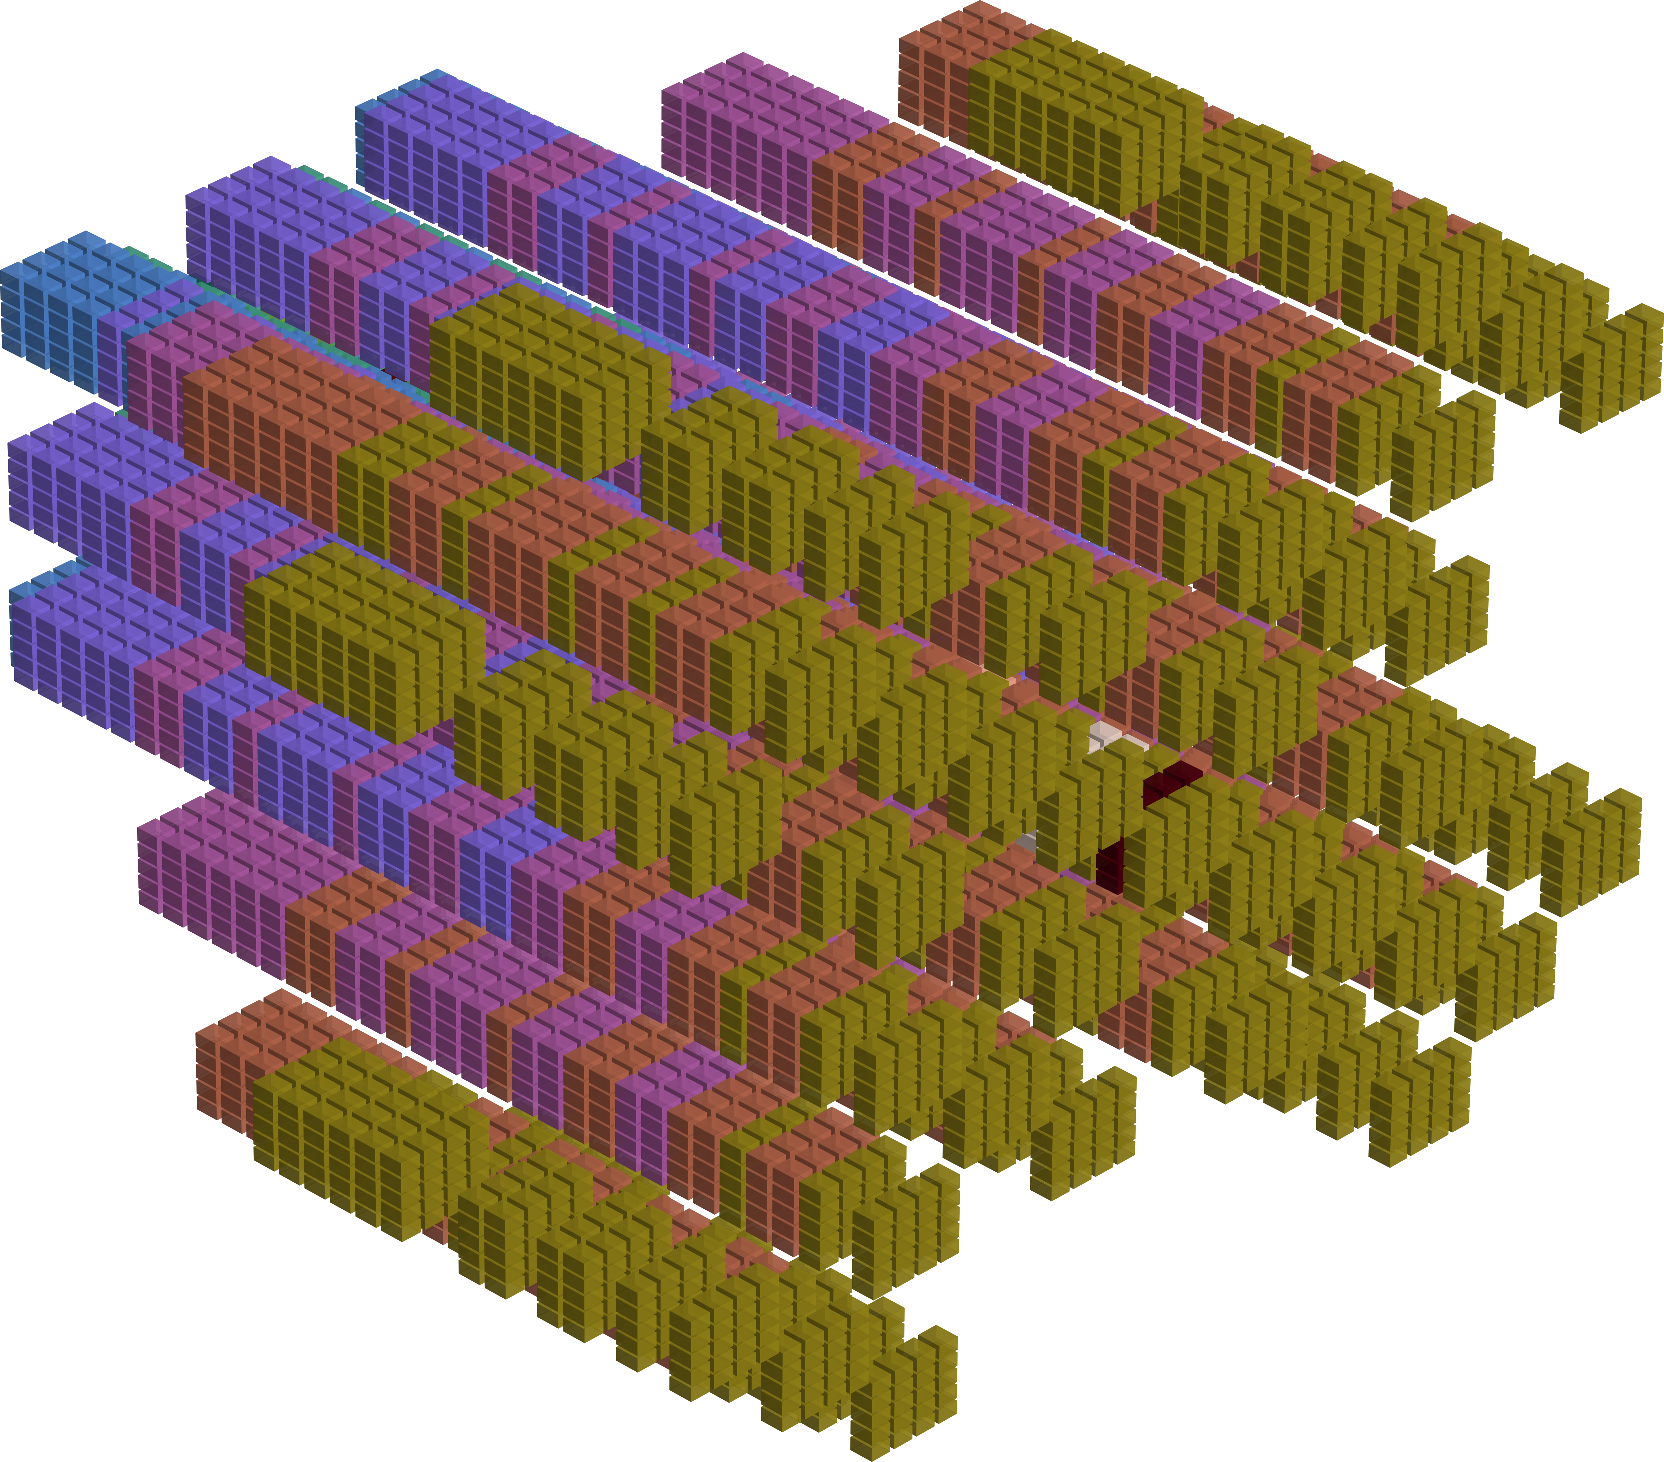
\includegraphics[width=10cm]{src/colorspace_patterns/pattern5-45.png}%
    \end{adjustbox}
    \begin{adjustbox}{width=5cm,margin=0cm 0cm}
      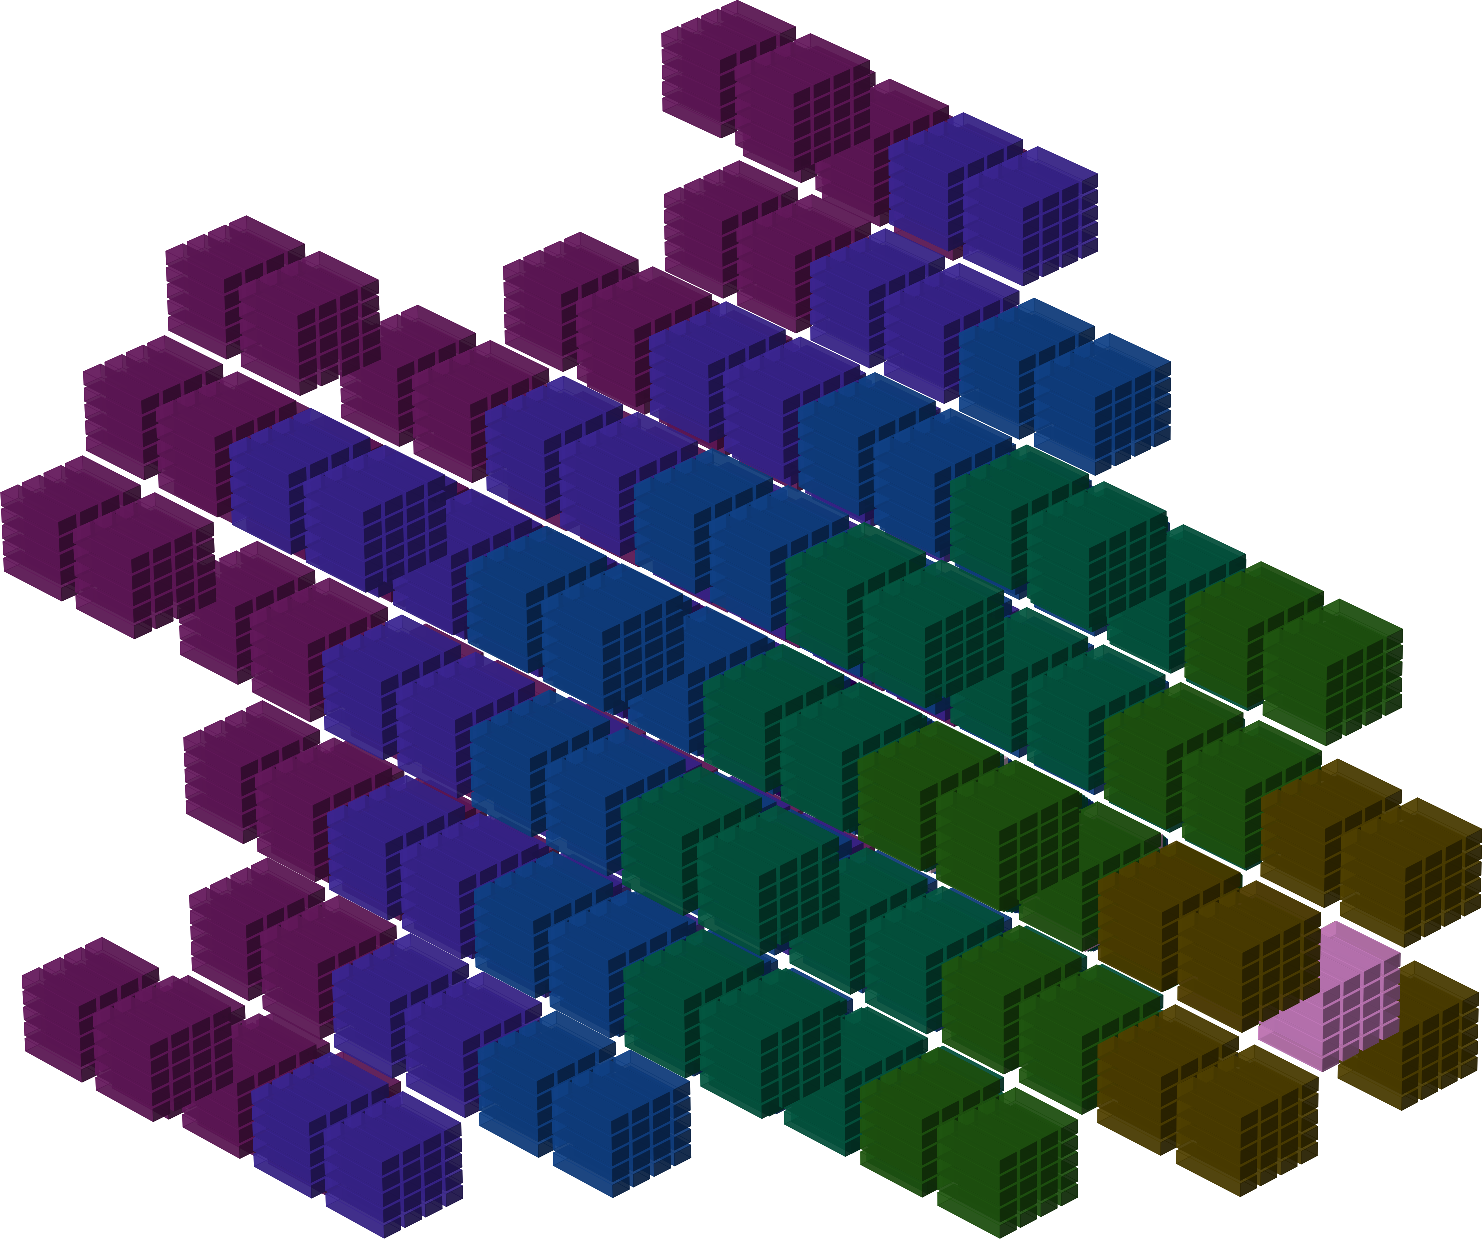
\includegraphics[width=10cm]{src/colorspace_patterns/pattern5-225.png}%
    \end{adjustbox}
\caption{'Sloth MultiCross'.}
\end{figure}
\end{minipage}
\begin{minipage}[b]{0.48\linewidth}
\begin{lrbox}{\mybox}%
\begin{lstlisting}[basicstyle=\ttfamily\tiny,escapechar=\%]
slothMultiCrossXPosArray
.BYTE $FF,$01,$01,$FF,$55                 ;   6     6  
.BYTE $FE,$02,$02,$FE,$55                 ;  5       5 
.BYTE $FD,$FF,$01,$03,$03,$01,$FF,$FD,$55 ; 6 4 3 3 4 6
.BYTE $FD,$03,$03,$FD,$55                 ;    2   2   
.BYTE $FC,$04,$04,$FC,$55                 ;   3 1 1 3  
.BYTE $FB,$FD,$03,$05,$05,$03,$FD,$FB,$55 ;            
.BYTE $55                                 ;   3 1 1 3  
slothMultiCrossYPosArray                  ;    2   2   
.BYTE $FF,$FF,$01,$01,$55                 ; 6 4 3 3 4 6
.BYTE $FE,$FE,$02,$02,$55                 ;  5       5 
.BYTE $FF,$FD,$FD,$FF,$01,$03,$03,$01,$55 ;   6     6  
.BYTE $FD,$FD,$03,$03,$55
.BYTE $FC,$FC,$04,$04,$55
.BYTE $FD,$FB,$FB,$FD,$03,$05,$05,$03,$55
.BYTE $55
\end{lstlisting}
\end{lrbox}%
\scalebox{0.8}{\usebox{\mybox}}
\subfile{colorspace_patterns/tables/pattern5.tex}
\end{minipage}
%
\begin{minipage}[b]{0.48\linewidth}
\vspace{0.5cm}
\begin{figure}[H]
    \centering
    \begin{adjustbox}{width=5cm,margin=0cm 0cm}
      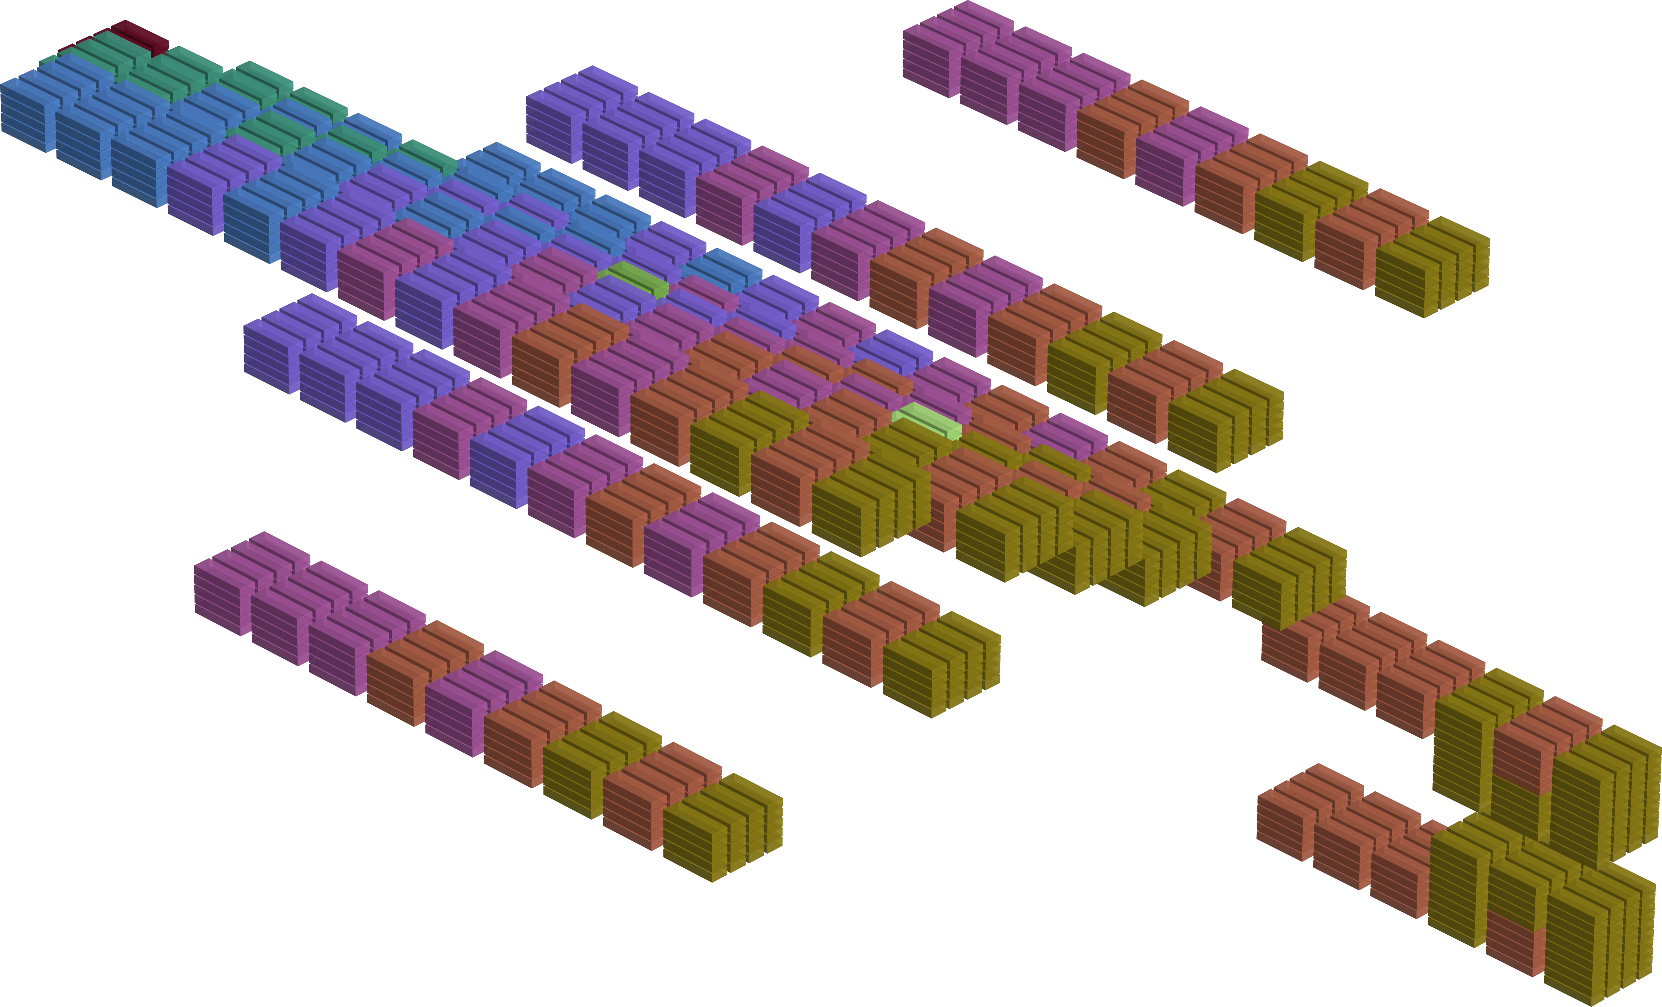
\includegraphics[width=10cm]{src/colorspace_patterns/pattern6-45.png}%
    \end{adjustbox}
    \begin{adjustbox}{width=5cm,margin=0cm 0cm}
      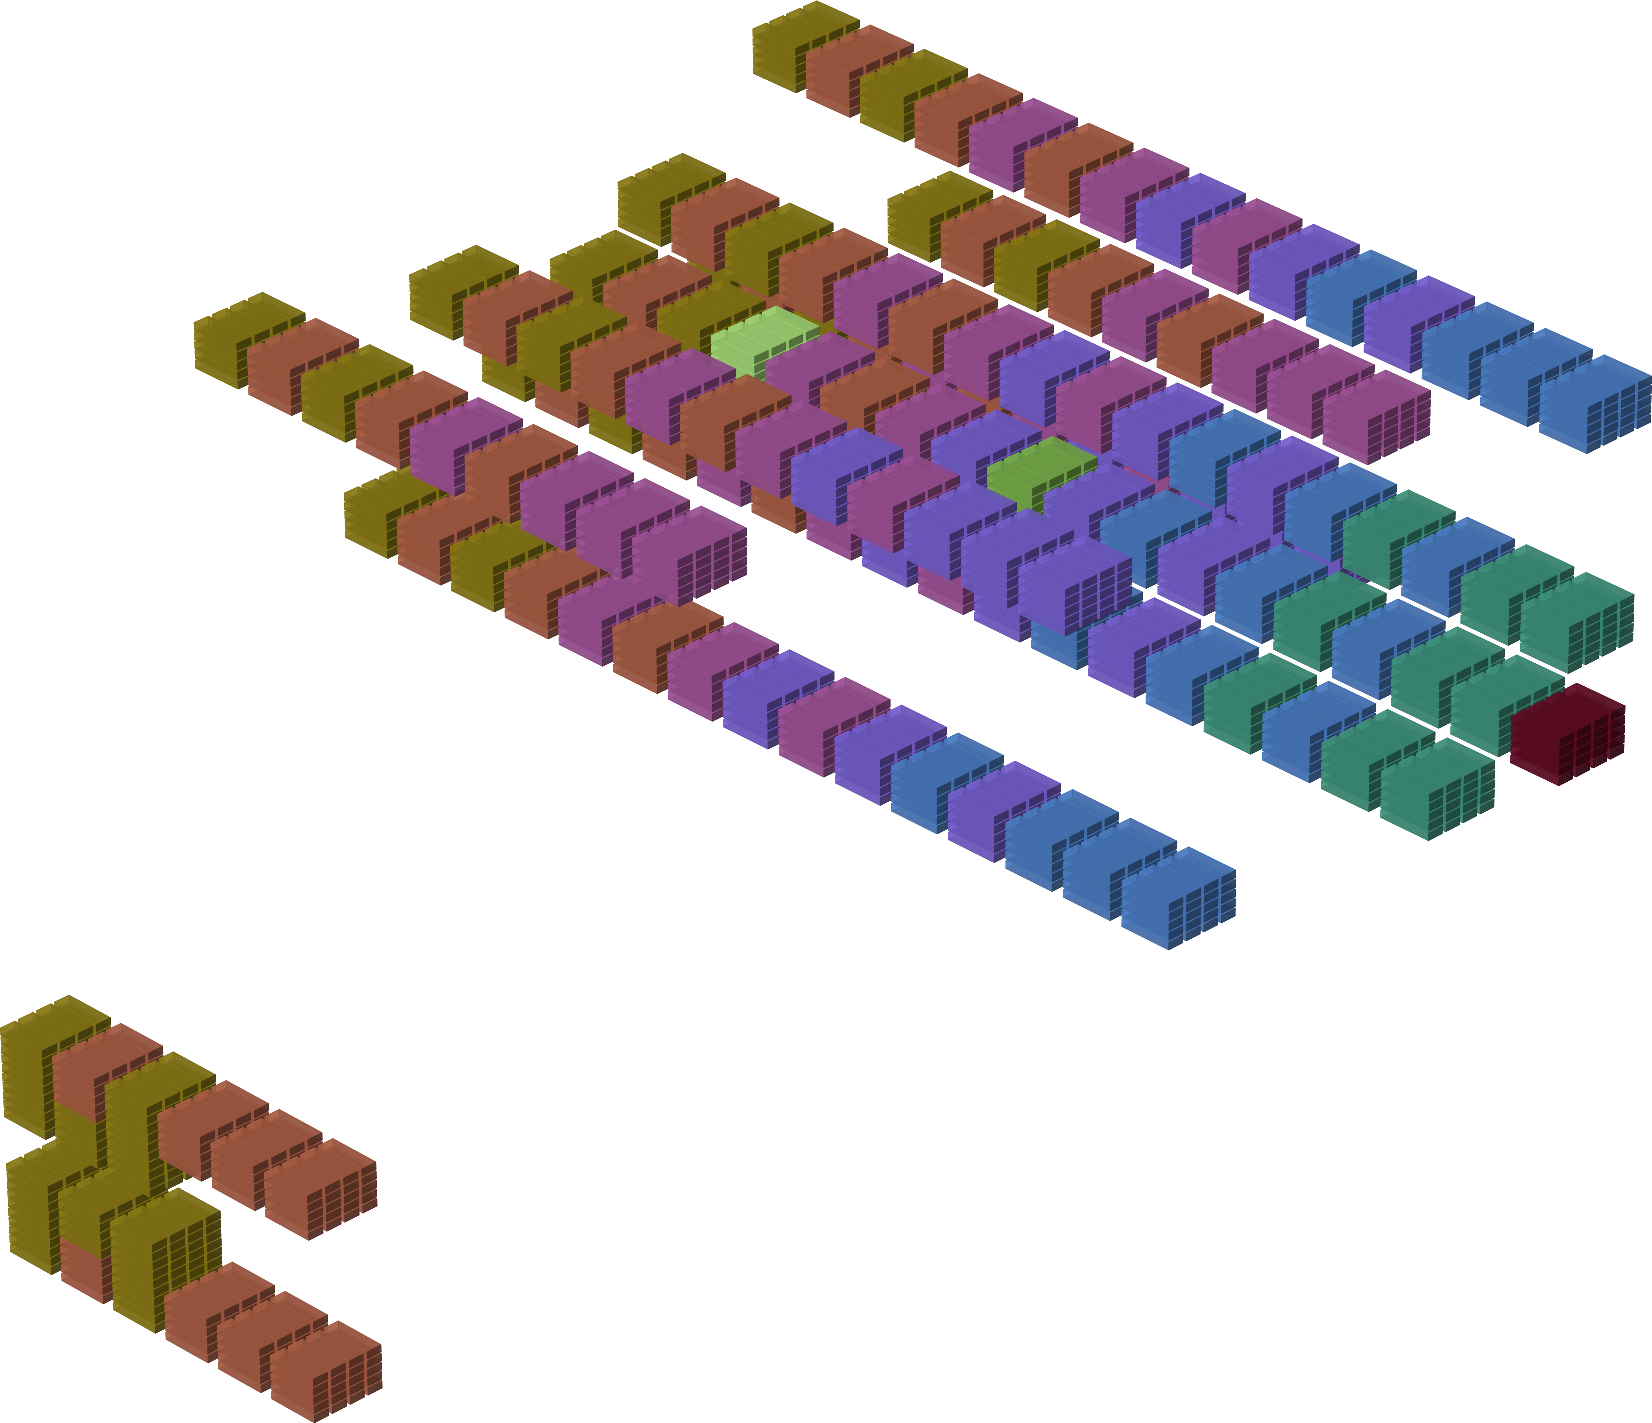
\includegraphics[width=10cm]{src/colorspace_patterns/pattern6-225.png}%
    \end{adjustbox}
\caption{'Cross And a Bit'.}
\end{figure}
\end{minipage}
\begin{minipage}[b]{0.48\linewidth}
\vspace{0.5cm}
\begin{lrbox}{\mybox}%
\begin{lstlisting}[basicstyle=\ttfamily\tiny,escapechar=\%]
crossAndABitXPosArray ;   2           
.BYTE $FF,$01,$55     ;           4   
.BYTE $FD,$03,$55     ;     1  3      
.BYTE $FE,$02,$55     ;               
.BYTE $FB,$05,$55     ;    3  1       
.BYTE $08,$08,$55     ; 4             
.BYTE $08,$08,$55     ;         2     
.BYTE $55             ;               
crossAndABitYPosArray ;               
.BYTE $FF,$01,$55     ;               
.BYTE $FD,$03,$55     ;               
.BYTE $01,$FF,$55     ;               
.BYTE $02,$FE,$55     ;               
.BYTE $0B,$0F,$55     ;               
.BYTE $0C,$0E,$55     ;              5
.BYTE $55             ;              6
                      ;               
                      ;              6
                      ;              5
\end{lstlisting}
\end{lrbox}%
\scalebox{0.8}{\usebox{\mybox}}
\subfile{colorspace_patterns/tables/pattern6.tex}
\end{minipage}
%
\begin{minipage}[b]{0.48\linewidth}
\begin{figure}[H]
    \centering
    \begin{adjustbox}{width=5cm,margin=0cm 0cm}
      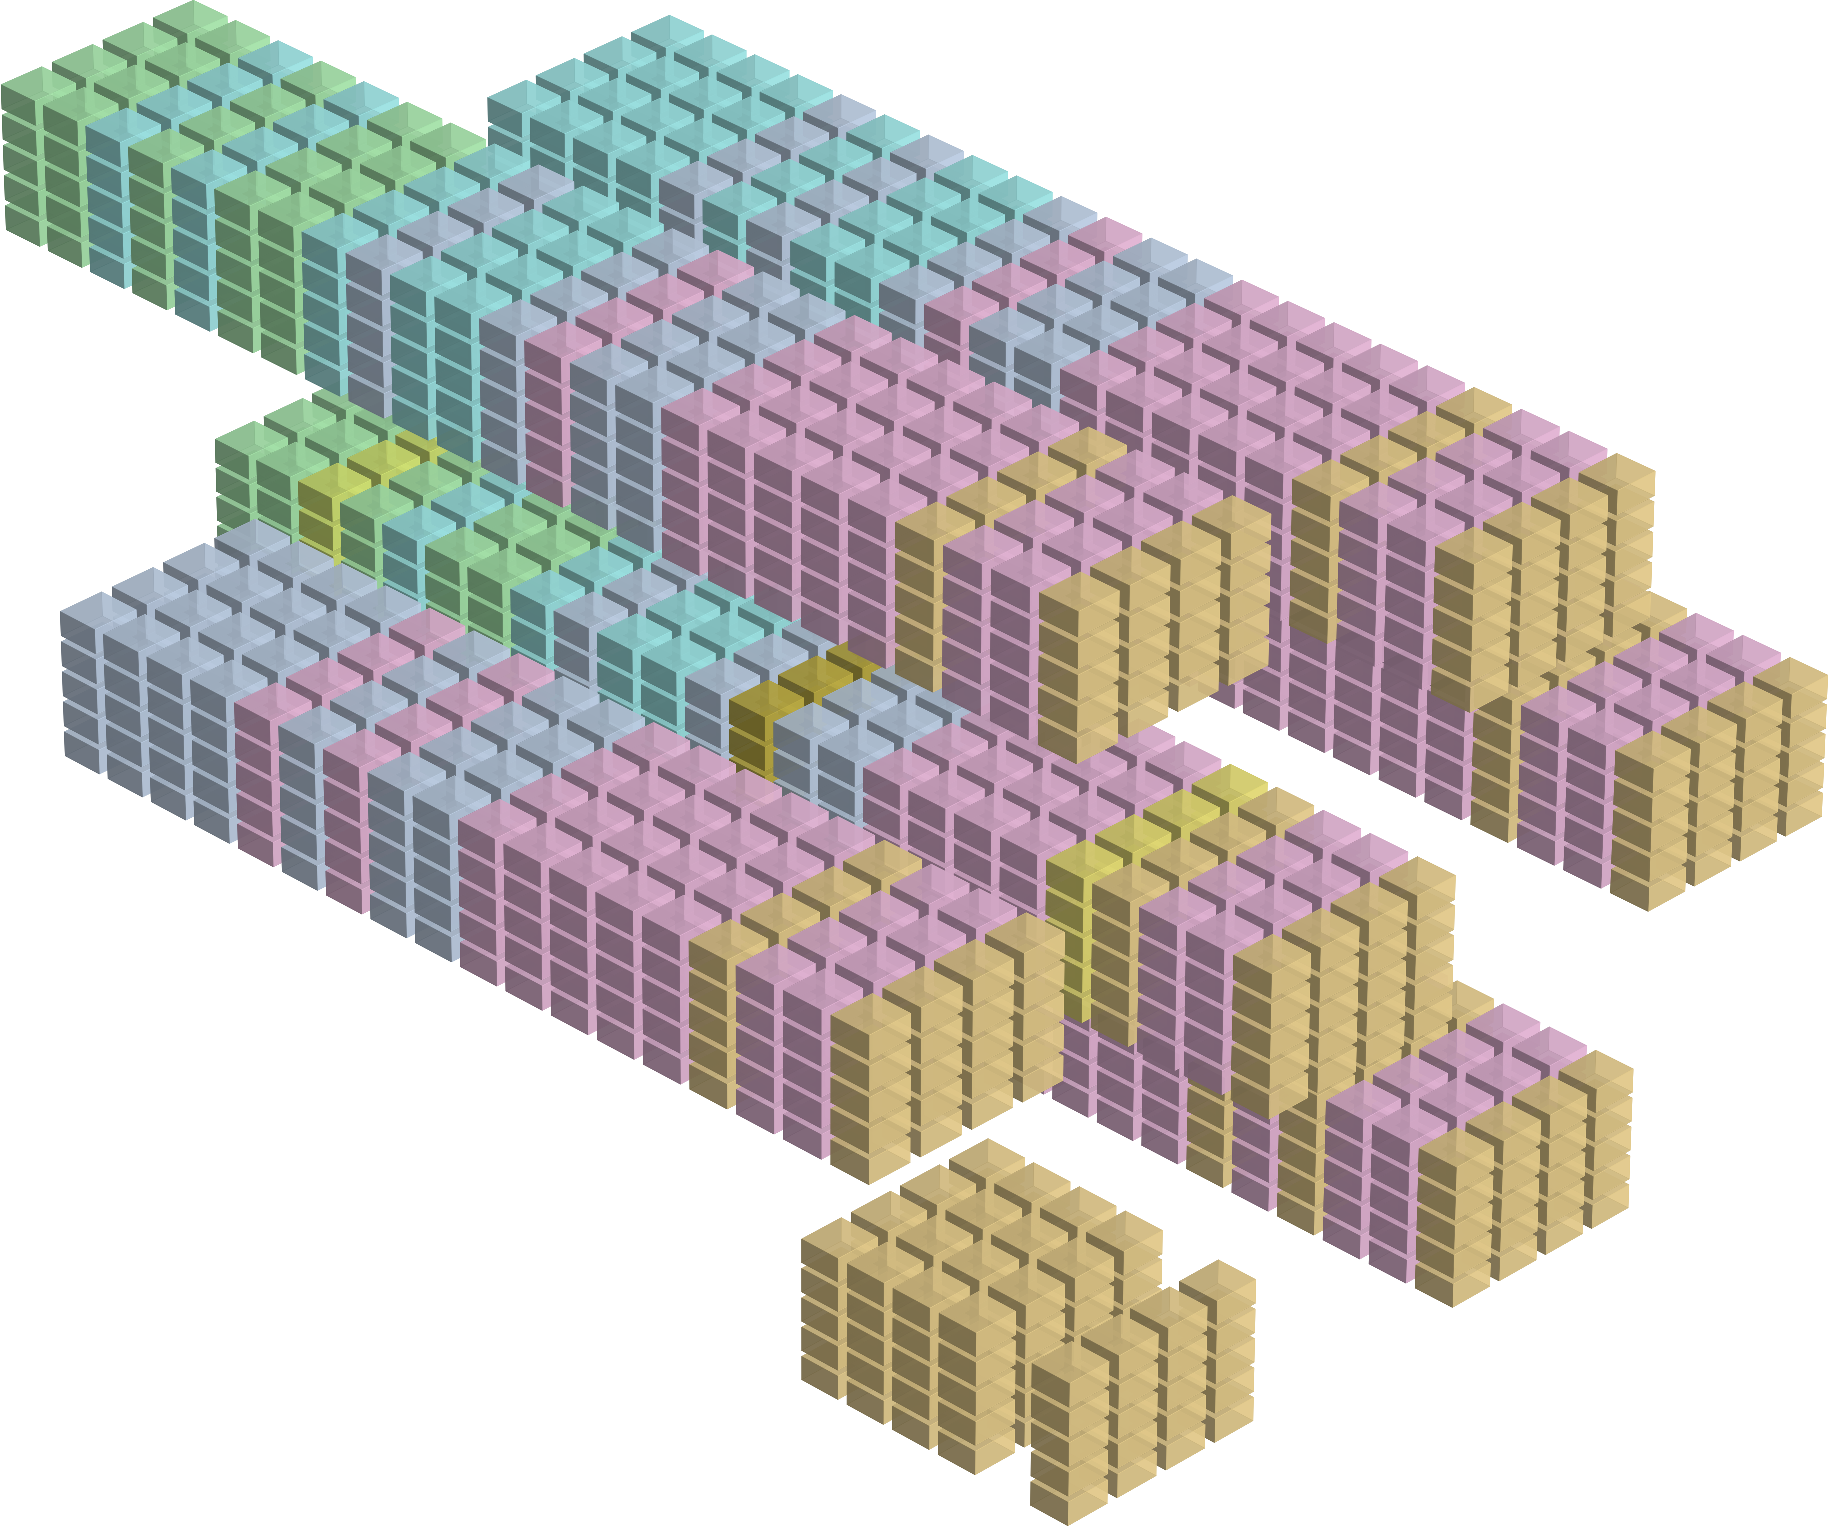
\includegraphics[width=10cm]{src/colorspace_patterns/pattern7-45.png}%
    \end{adjustbox}
    \begin{adjustbox}{width=5cm,margin=0cm 0cm}
      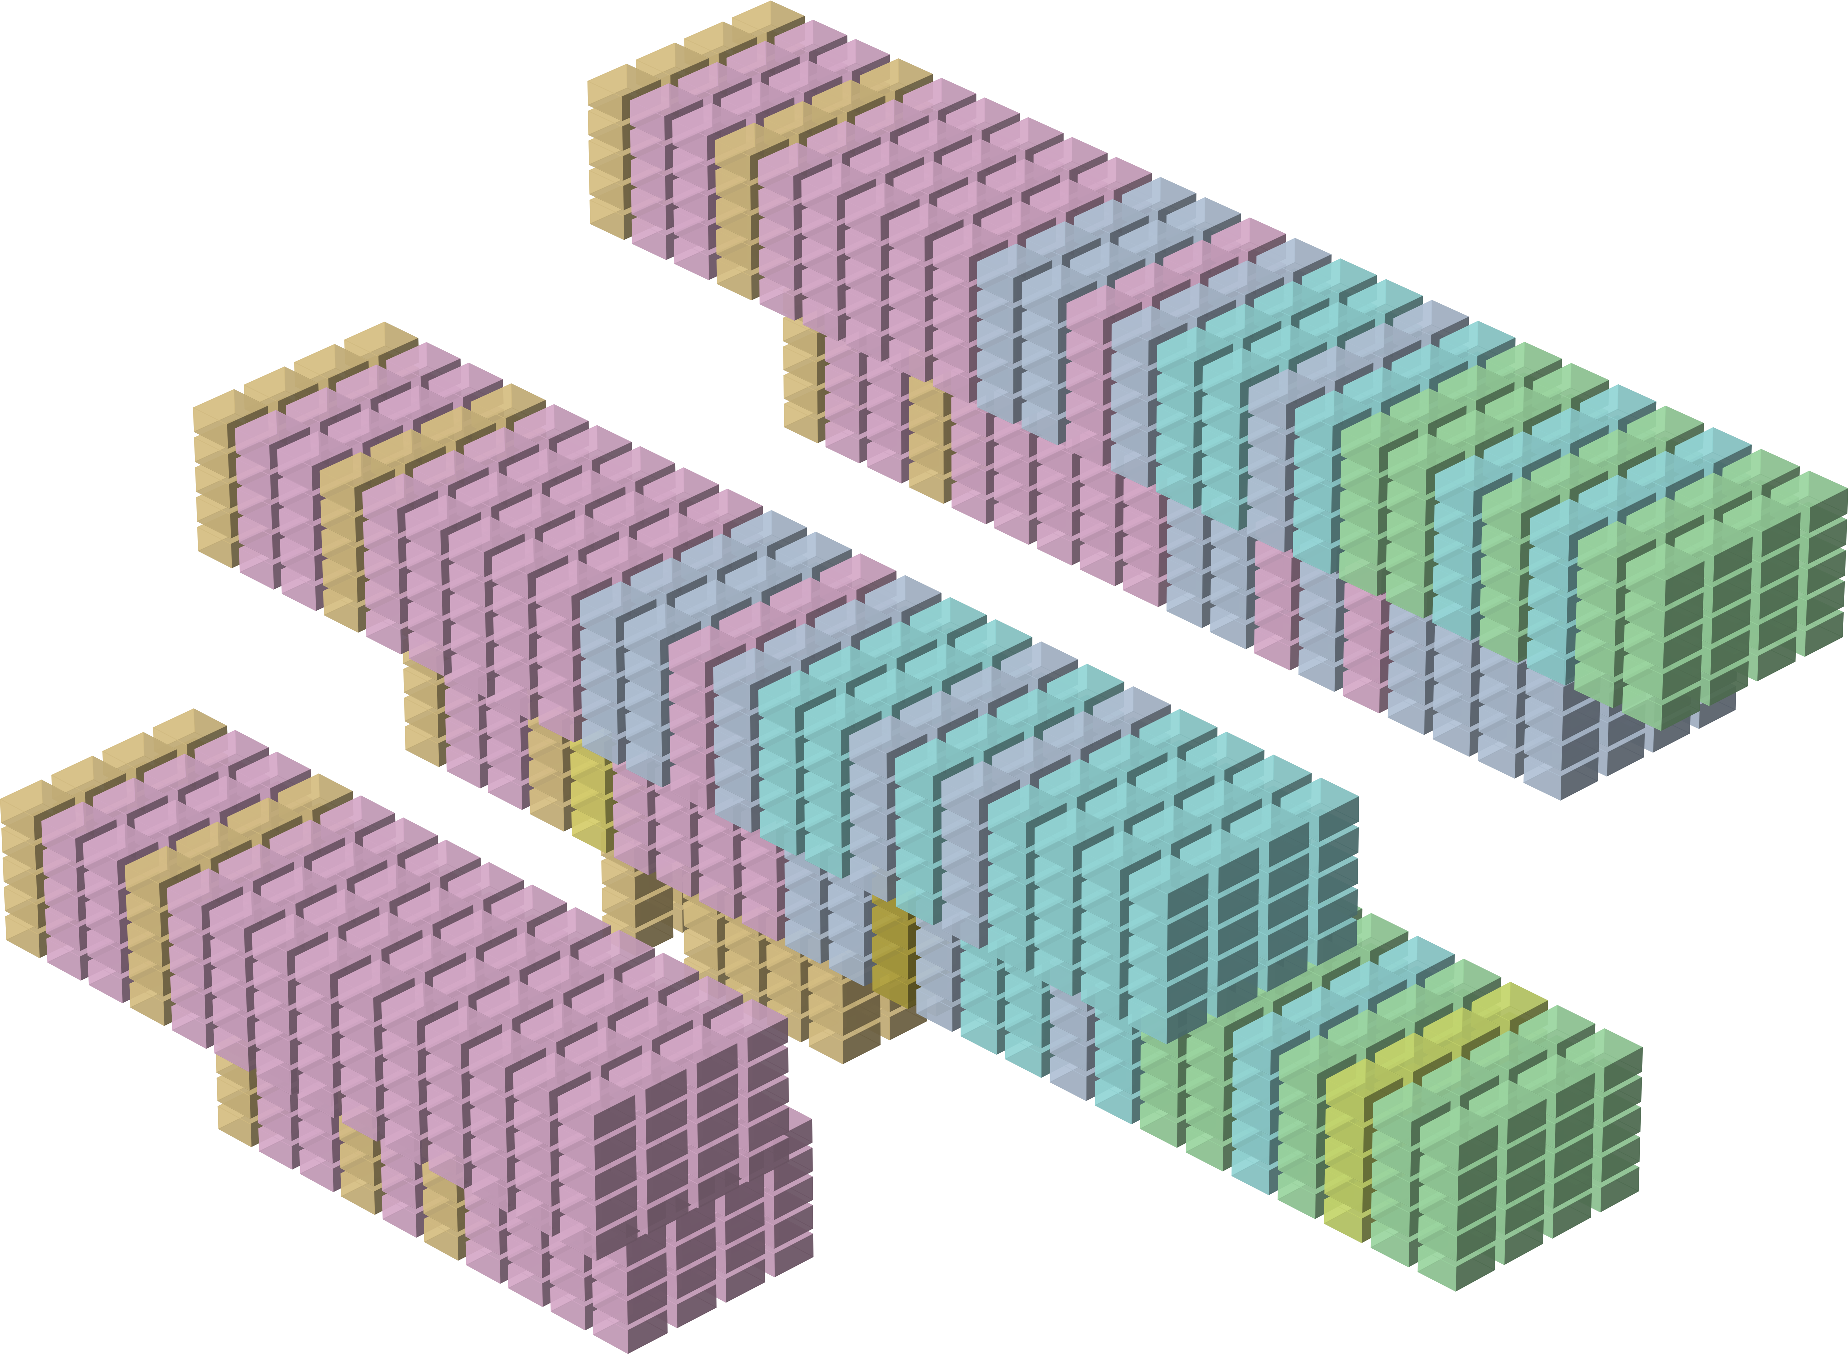
\includegraphics[width=10cm]{src/colorspace_patterns/pattern7-225.png}%
    \end{adjustbox}
\caption{'Star Two'.}
\end{figure}
\end{minipage}
\begin{minipage}[b]{0.48\linewidth}
\begin{lrbox}{\mybox}%
\begin{lstlisting}[basicstyle=\ttfamily\tiny,escapechar=\%]
star2XPosArray
  .BYTE $FF,$55  ;  1   
  .BYTE $01,$55  ;    2 
  .BYTE $FE,$55  ; 3    
  .BYTE $02,$55  ;     4
  .BYTE $01,$55  ;      
  .BYTE $FF,$55  ;  6 5 
  .BYTE $55
start2YPosArray
  .BYTE $FD,$55
  .BYTE $FE,$55
  .BYTE $FF,$55
  .BYTE $00,$55
  .BYTE $02,$55
  .BYTE $02,$55
  .BYTE $55
\end{lstlisting}
\end{lrbox}%
\scalebox{0.8}{\usebox{\mybox}}
\subfile{colorspace_patterns/tables/pattern7.tex}
\end{minipage}
%
\begin{minipage}[b]{0.48\linewidth}
\vspace{1cm}
\begin{figure}[H]
    \centering
    \begin{adjustbox}{width=4cm,margin=0cm 0cm}
      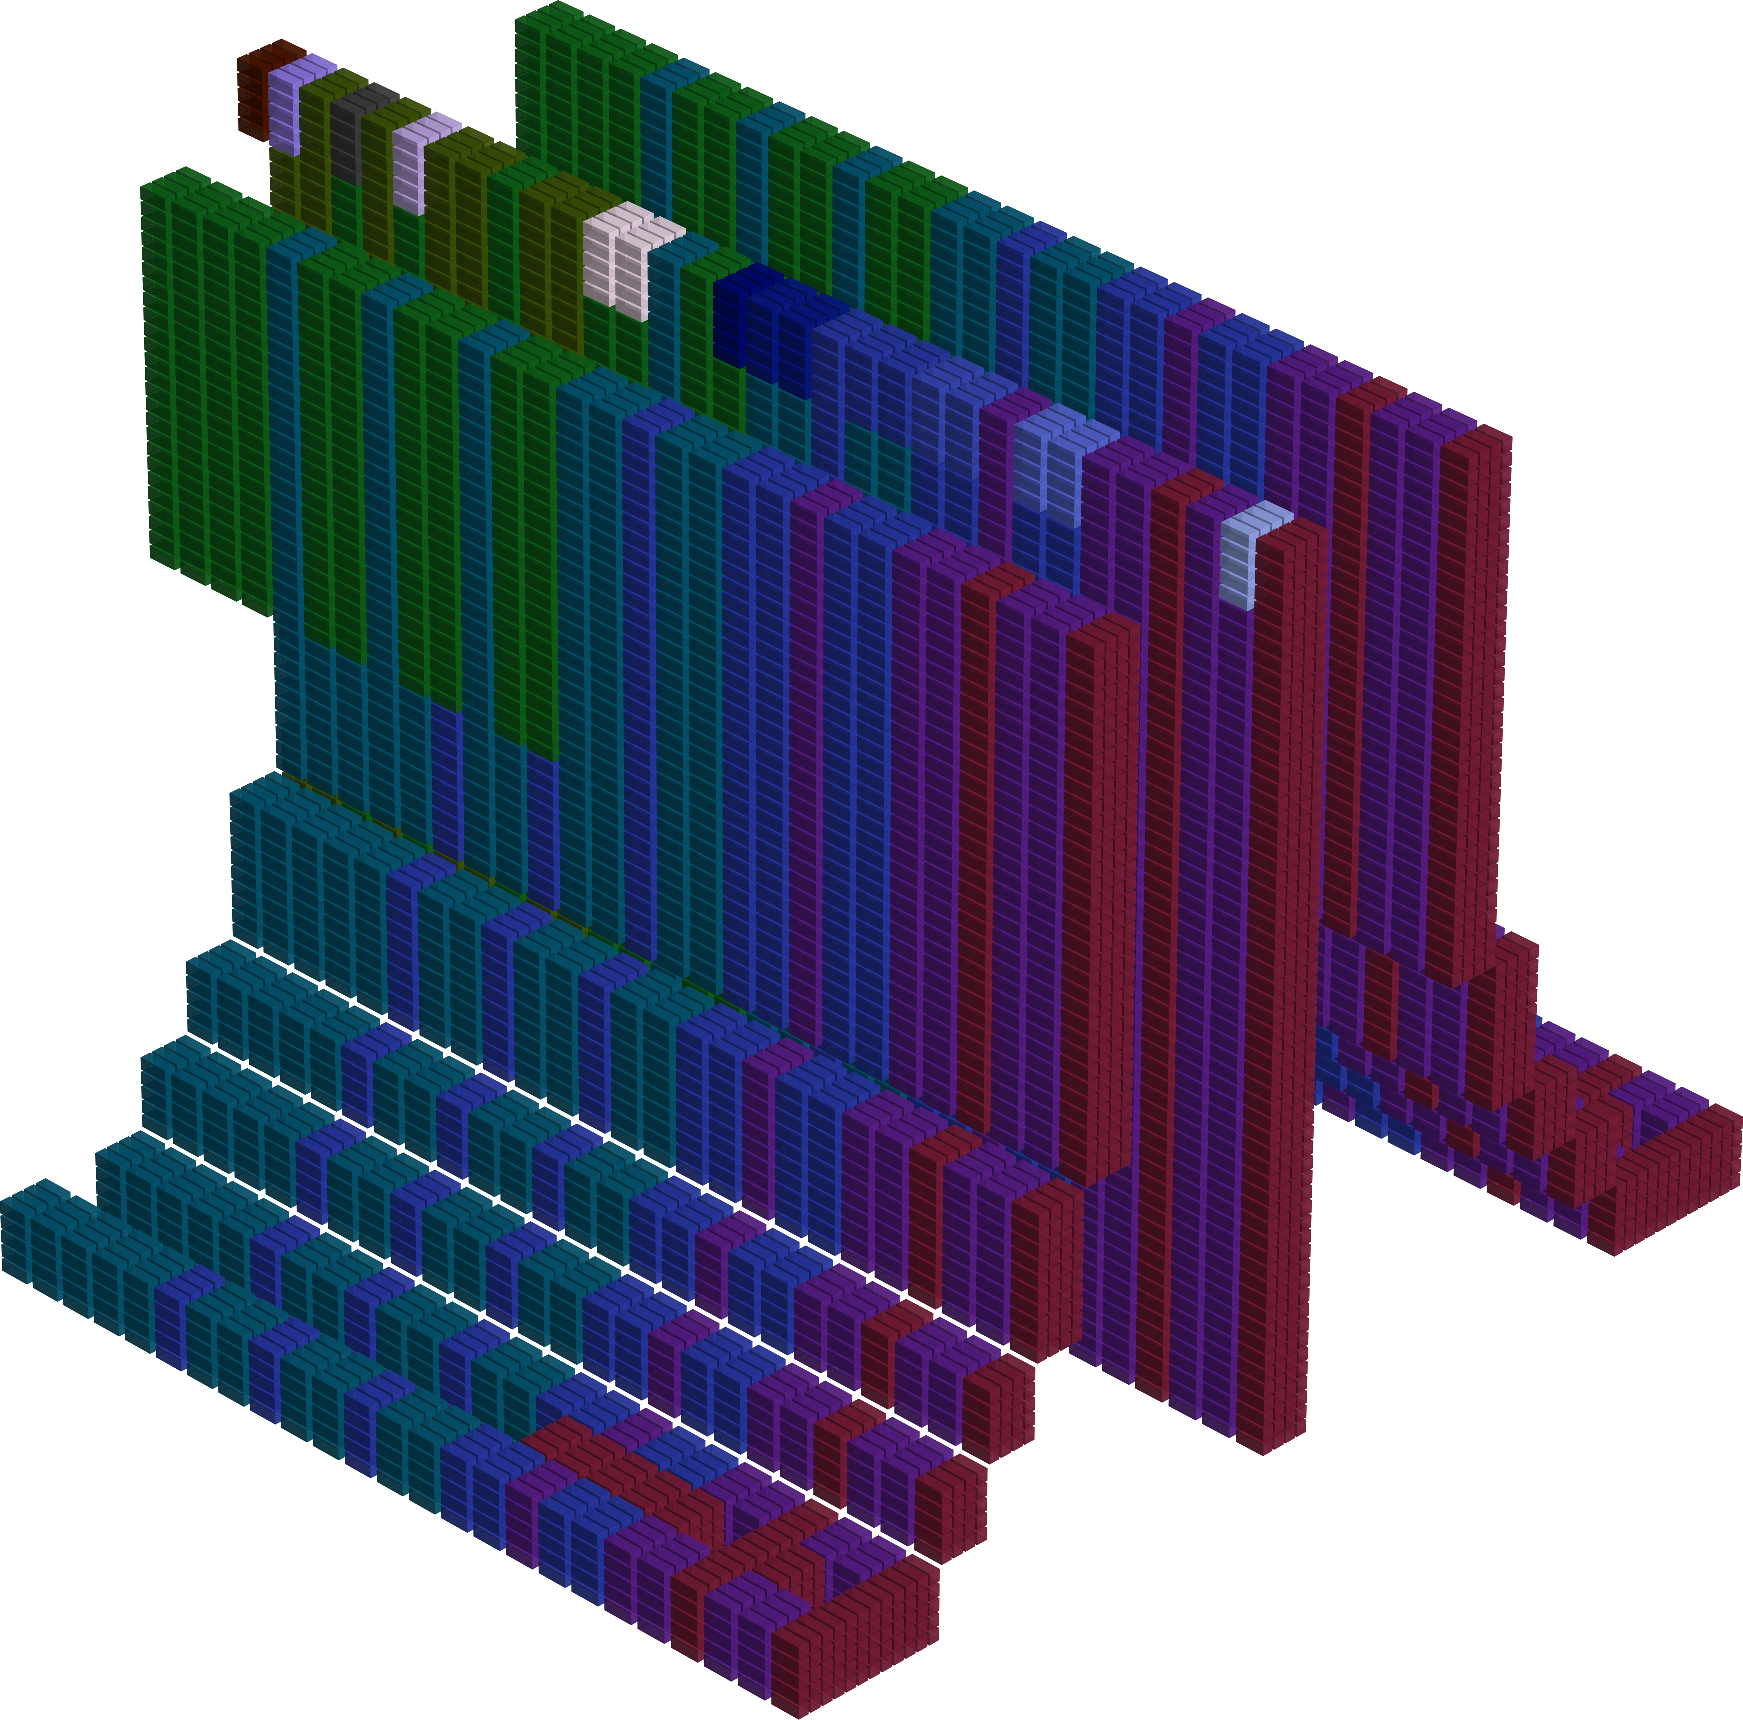
\includegraphics[width=10cm]{src/colorspace_patterns/pattern8-45.png}%
    \end{adjustbox}
    \begin{adjustbox}{width=4cm,margin=0cm 0cm}
      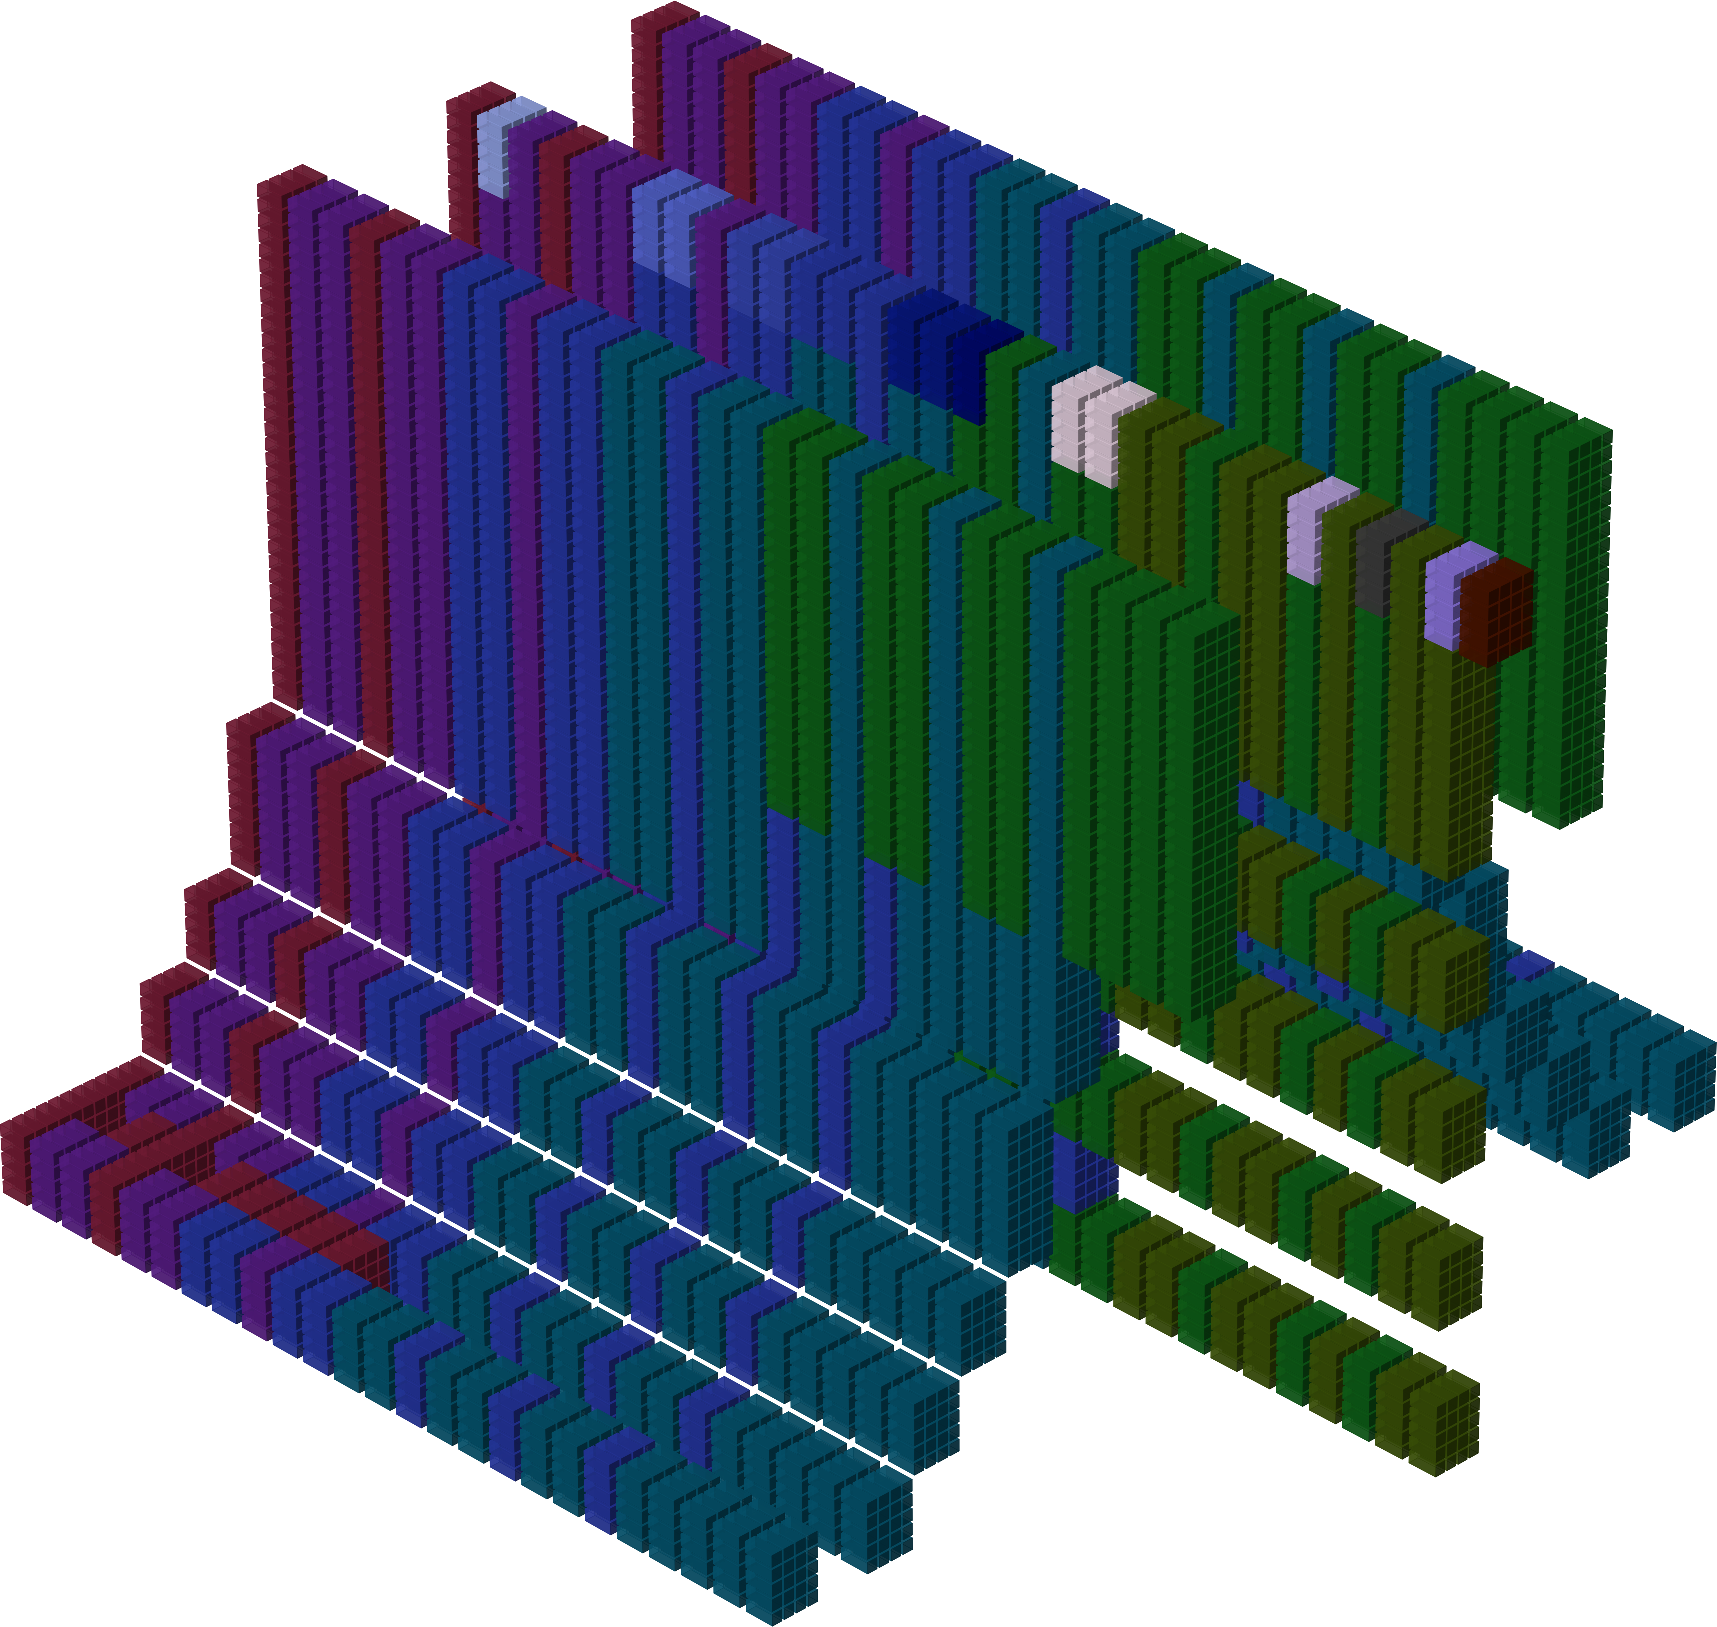
\includegraphics[width=10cm]{src/colorspace_patterns/pattern8-225.png}%
    \end{adjustbox}
\caption{'User LightForm 0'.}
\end{figure}
\end{minipage}
\begin{minipage}[b]{0.48\linewidth}
\vspace{1cm}
\begin{lrbox}{\mybox}%
\hspace{1cm}
\begin{lstlisting}[basicstyle=\ttfamily\tiny,escapechar=\%]
userLightform0XPosArray
  .BYTE $00,$00,$00,$00,$00,$00,$00,$55                                        ;       2       2      
  .BYTE $04,$04,$04,$04,$04,$FC,$FC,$FC,$FC,$FC,$55                            ;       2   1   2      
  .BYTE $FC,$FC,$FB,$FB,$FA,$F9,$F8,$F6,$04,$04,$05,$05,$06,$07,$08,$0A,$55    ;       2   1   2      
  .BYTE $00,$00,$00,$55                                                        ;       2   1   2      
  .BYTE $00,$55                                                                ;       2   5   2      
  .BYTE $F7,$09,$55                                                            ;       3   1   3      
  .BYTE $55                                                                    ;       3   4   3      
userLightform0YPosArray                                                        ;      3    1    3     
  .BYTE $01,$03,$02,$05,$07,$09,$0B,$07                                        ;      3    4    3     
  .BYTE $00,$01,$02,$03,$04,$00,$01,$02,$03,$04,$03                            ;     3     1     3    
  .BYTE $05,$06,$07,$08,$09,$0A,$0B,$0B,$05,$06,$07,$08,$09,$0A,$0B,$0B,$03    ;    3      4      3   
  .BYTE $0A,$08,$06,$01                                                        ; 363       1       363
  .BYTE $04,$FF
  .BYTE $0B,$0B,$07
  .BYTE $09,$09,$55                                                         
  .BYTE $55
\end{lstlisting}
\end{lrbox}%
\scalebox{0.8}{\usebox{\mybox}}
\subfile{colorspace_patterns/tables/pattern8.tex}
\end{minipage}
%
\clearpage
\textbf{Lines 1189-1231. \icode{\textbf{PaintPixelForCurrentSymmetry}}} 
\begin{lstlisting}[basicstyle=\ttfamily\tiny, caption=The routine responsible for painting patterns.]
PaintPixelForCurrentSymmetry
        LDA currentPaintState
        PHA 
        JSR PaintPixel
        LDA currentSymmetrySetting
        BNE b4279
        PLA 
        RTS 

b4279   CMP #E_Y_AXIS_SYMMETRY
        BNE MaybeXYSymmetry

YAxisSymmetry
        LDA #NUM_COLS-1
        SEC 
        SBC previousPixelXPosition
        STA previousPixelXPosition
        PLA 
        JMP PaintPixel

MaybeXYSymmetry   
        CMP #E_X_Y_SYMMETRY
        BNE MaybeXAxisSymmetry

        ; X-Y Symmetry
        LDA currentBottomMostYPos
        SEC 
        SBC previousPixelYPosition
        STA previousPixelYPosition
        JMP YAxisSymmetry

MaybeXAxisSymmetry   
        CMP #E_X_AXIS_SYMMETRY
        BNE QuadSymmetry

        LDA currentBottomMostYPos
        SEC 
        SBC previousPixelYPosition
        STA previousPixelYPosition
        PLA 
        JMP PaintPixel

QuadSymmetry   
        LDA currentBottomMostYPos
        SEC 
        SBC previousPixelYPosition
        STA previousPixelYPosition
        PLA 
        PHA 

        JSR PaintPixel

        LDA #NUM_COLS-1
        SEC 
        SBC previousPixelXPosition
        STA previousPixelXPosition
        PLA 
        PHA 

        JSR PaintPixel

        LDA currentBottomMostYPos
        SEC 
        SBC previousPixelYPosition
        STA previousPixelYPosition
        PLA 

        JMP PaintPixel
\end{lstlisting}
\clearpage

\rhead[]{\icode{PaintPixelForCurrentSymmetry}}
\textbf{Lines 1189-1231. \icode{\textbf{PaintPixelForCurrentSymmetry}}:} We've already encountered this routine
in \hyperref[sec:listing_commentary]{\textcolor{blue}{ our walk through of the listing.}}. This is the version that shipped 
with the commercial edition of Psychedelia so has a necessary extra complication to deal with the fact that we 
are going to paint one of up to 16 possible patterns. What we want to figure out here is the X and Y position we should
paint for each element in the pattern's data structure.
\clearpage

%
\begin{minipage}[b]{0.48\linewidth}
\begin{figure}[H]
    \centering
    \begin{adjustbox}{width=5cm,margin=0cm 0cm}
      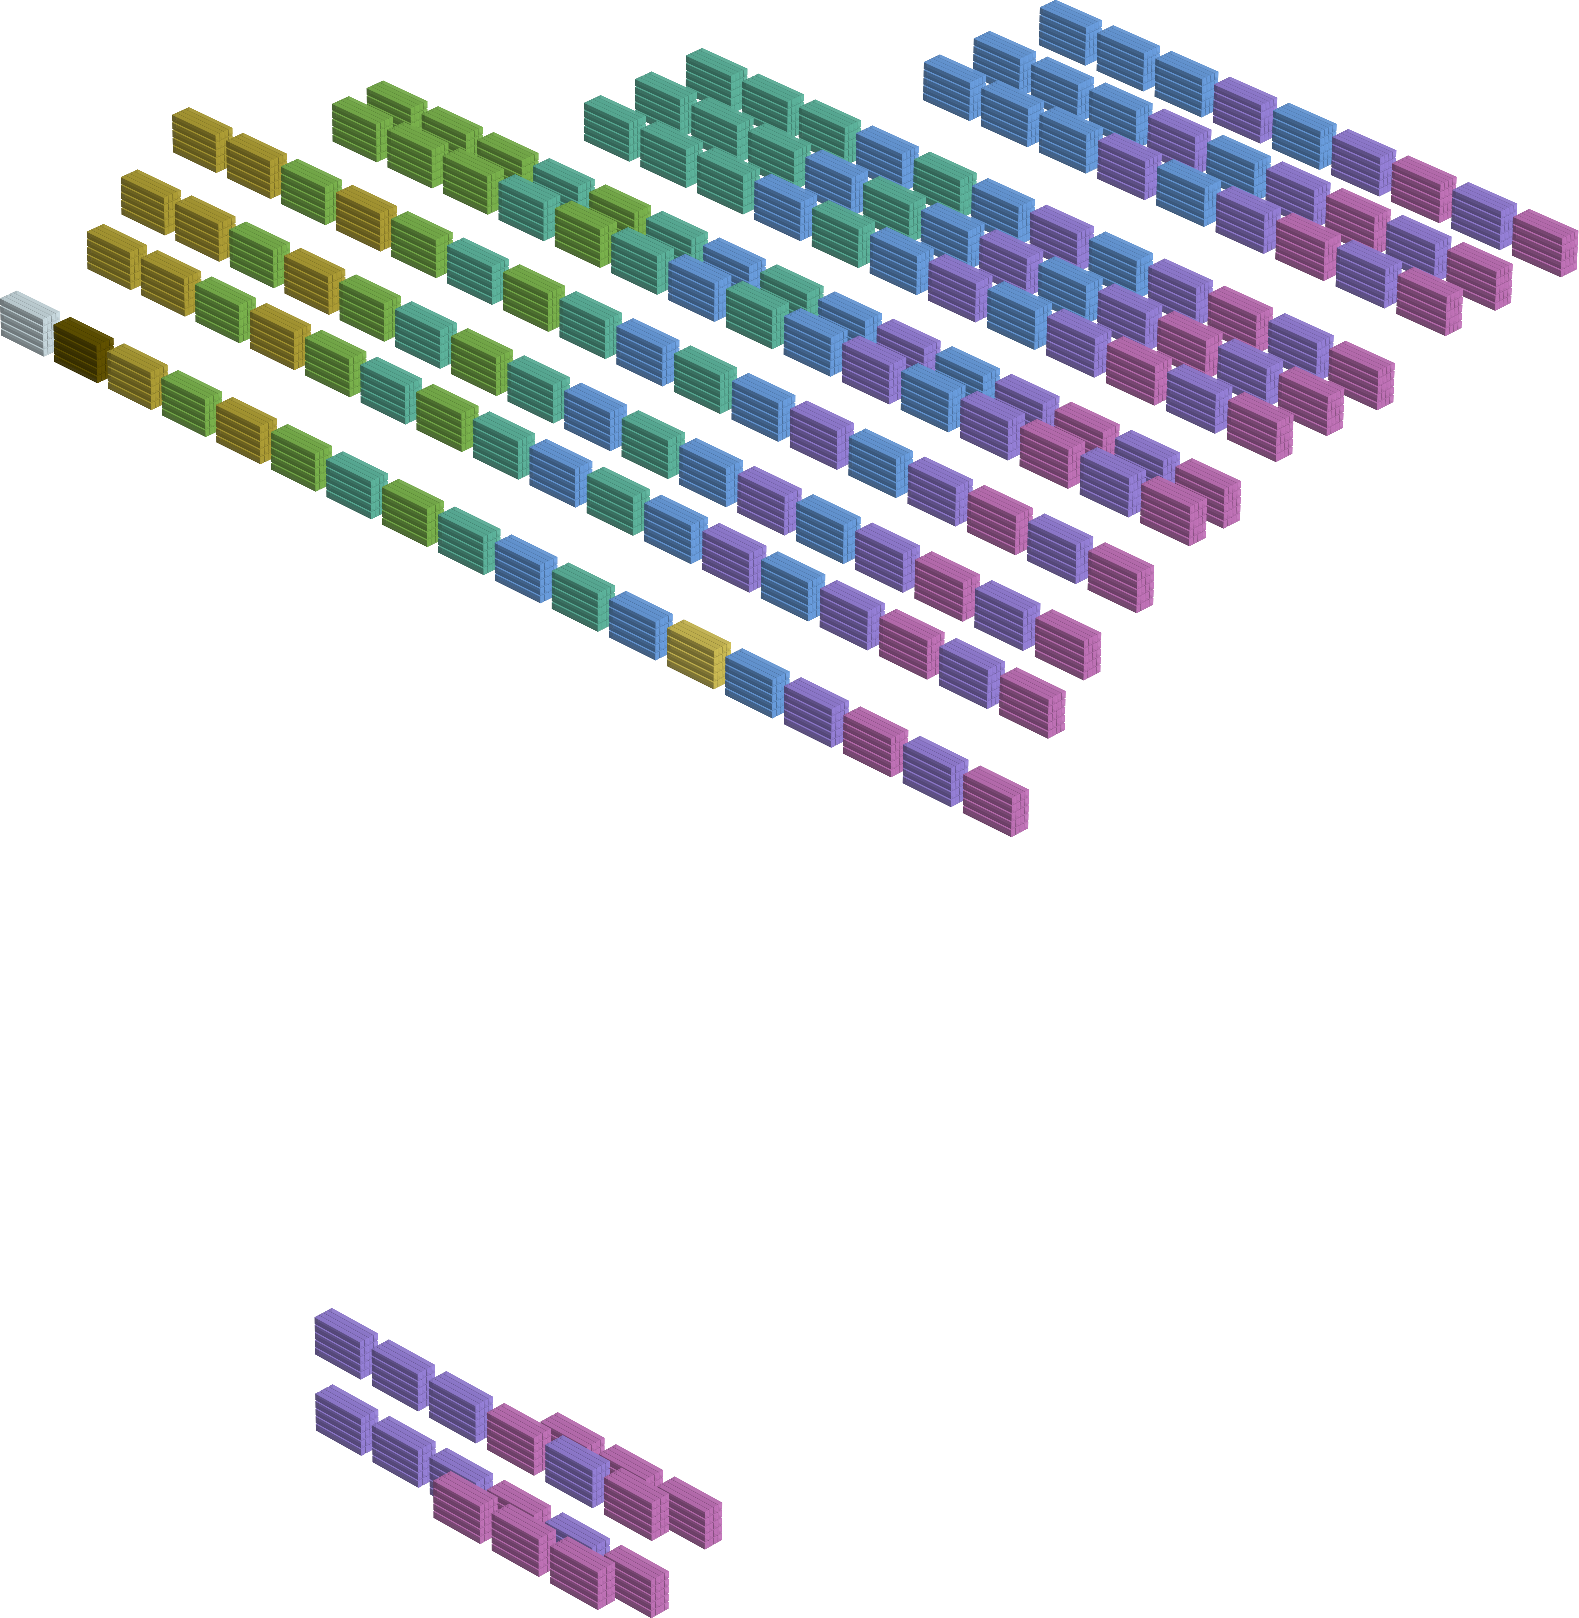
\includegraphics[width=10cm]{src/colorspace_patterns/pattern9-45.png}%
    \end{adjustbox}
    \begin{adjustbox}{width=5cm,margin=0cm 0cm}
      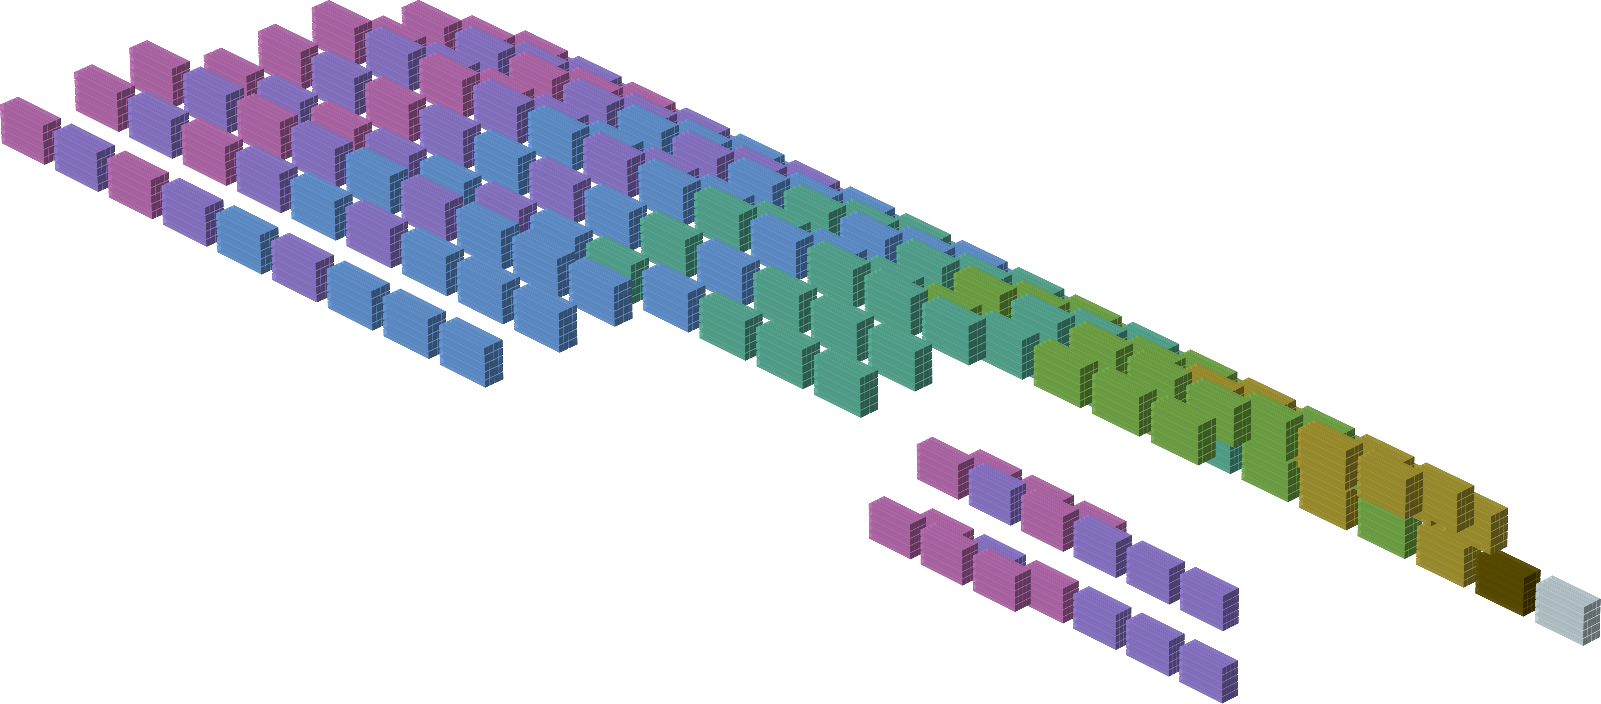
\includegraphics[width=10cm]{src/colorspace_patterns/pattern9-225.png}%
    \end{adjustbox}
\caption{'User LightForm 1'.}
\end{figure}
\end{minipage}
\begin{minipage}[b]{0.48\linewidth}
\begin{lrbox}{\mybox}%
\hspace{1cm}
\begin{lstlisting}[basicstyle=\ttfamily\tiny,escapechar=\%]
userLightform1XPosArray
  .BYTE $02,$04,$07,$55   ;                                                 4  4   4
  .BYTE $0A,$0C,$55       ;                                       3  3  3           
  .BYTE $0F,$12,$15,$55   ;                                  2 2                    
  .BYTE $19,$1C,$20,$55   ;                               1                         
  .BYTE $EC,$EC,$55       ;                            1                            
  .BYTE $E9,$EF,$55       ;                          1                              
  .BYTE $55               ;                                                         
userLightform1YPosArray
  .BYTE $FE,$FD,$FC,$FC   ;        
  .BYTE $FB,$FB,$FB       ;        
  .BYTE $FA,$FA,$FA,$55   ;        
  .BYTE $F9,$F9,$F9,$55   ;        
  .BYTE $0D,$0F,$55       ;        
  .BYTE $0E,$0E,$55       ;        
  .BYTE $55               ;        
                          ;        
                          ;        
                          ;        
                          ;        
                          ;        
                          ;    5   
                          ; 6     6
                          ;    5   
\end{lstlisting}
\end{lrbox}%
\scalebox{0.8}{\usebox{\mybox}}
\subfile{colorspace_patterns/tables/pattern9.tex}
\end{minipage}
%
%
\begin{minipage}[b]{0.48\linewidth}
\vspace{0.5cm}
\begin{figure}[H]
    \centering
    \begin{adjustbox}{width=4cm,margin=0cm 0cm}
      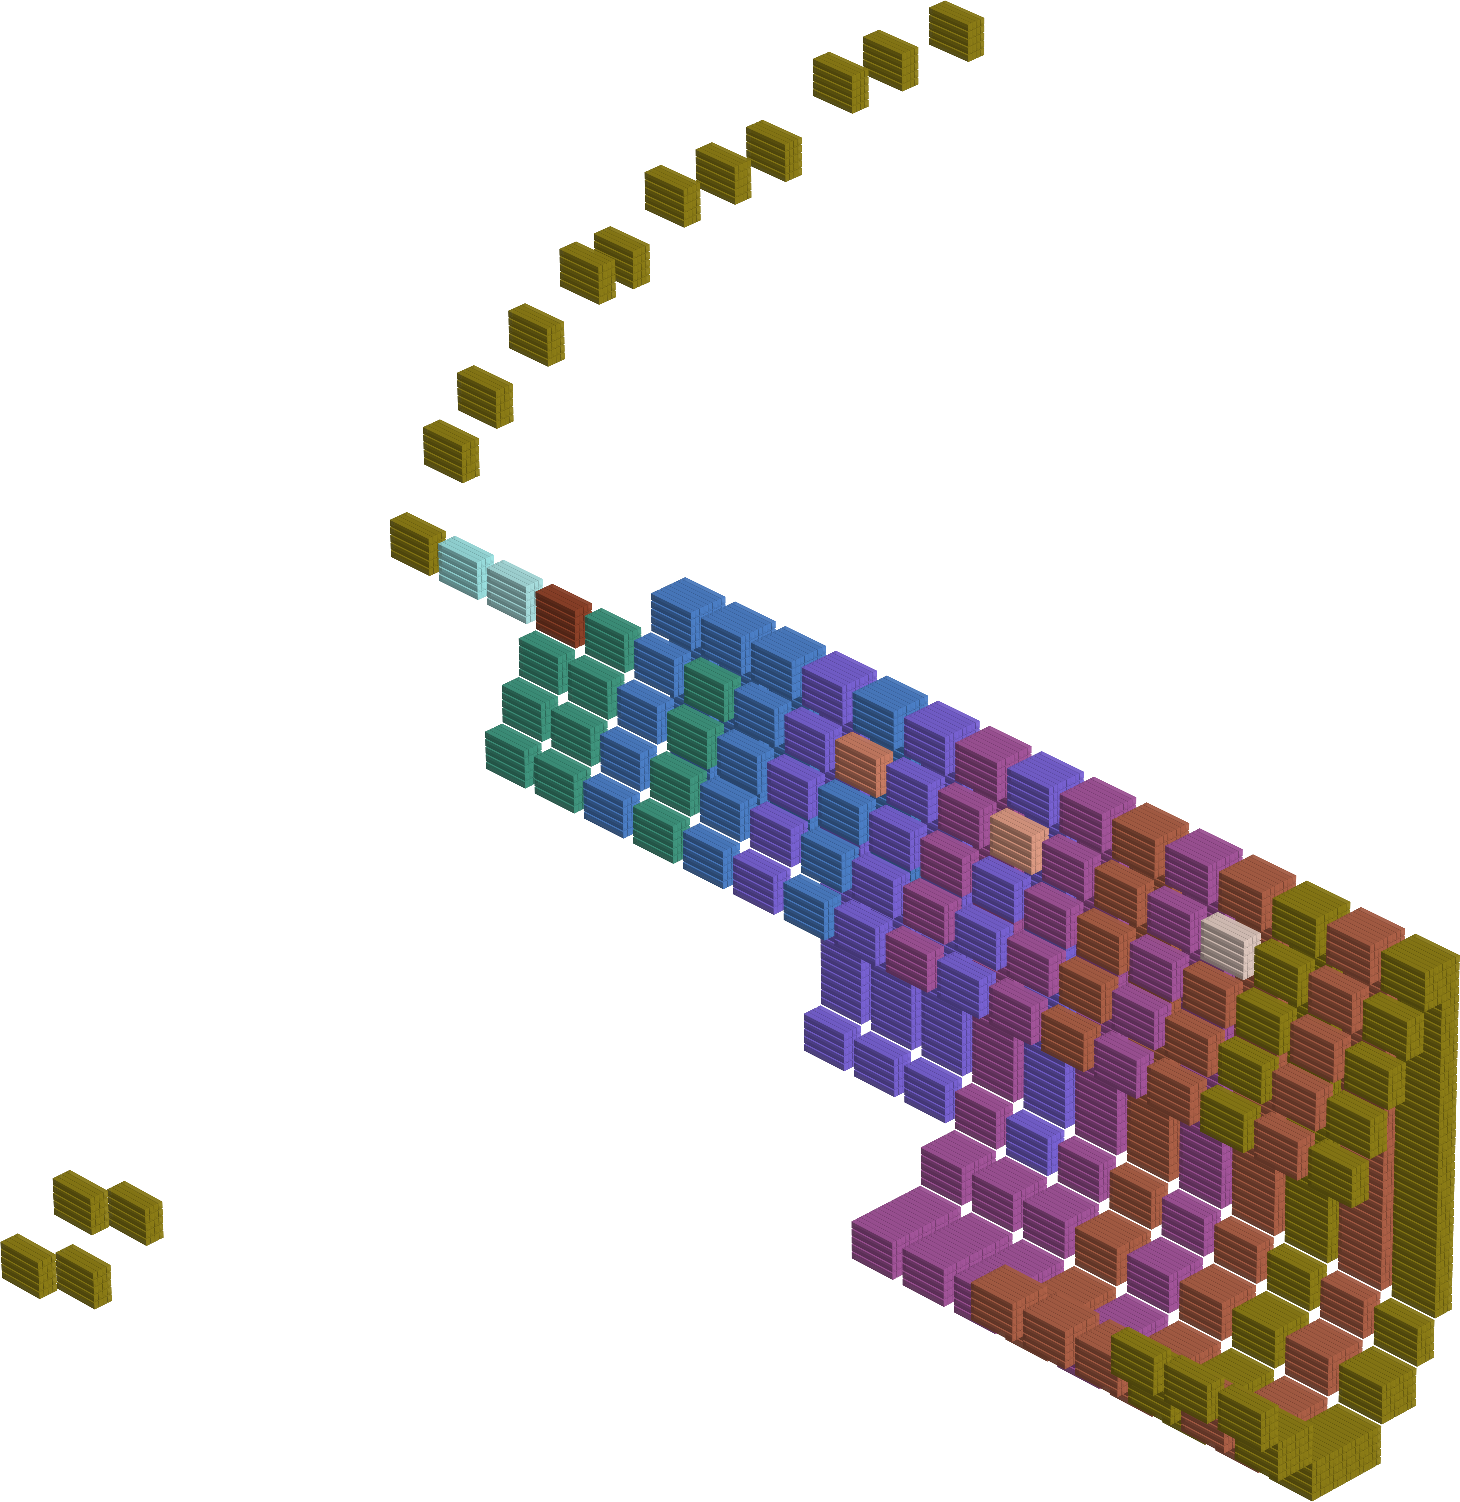
\includegraphics[width=10cm]{src/colorspace_patterns/pattern10-45.png}%
    \end{adjustbox}
    \begin{adjustbox}{width=5cm,margin=0cm 0cm}
      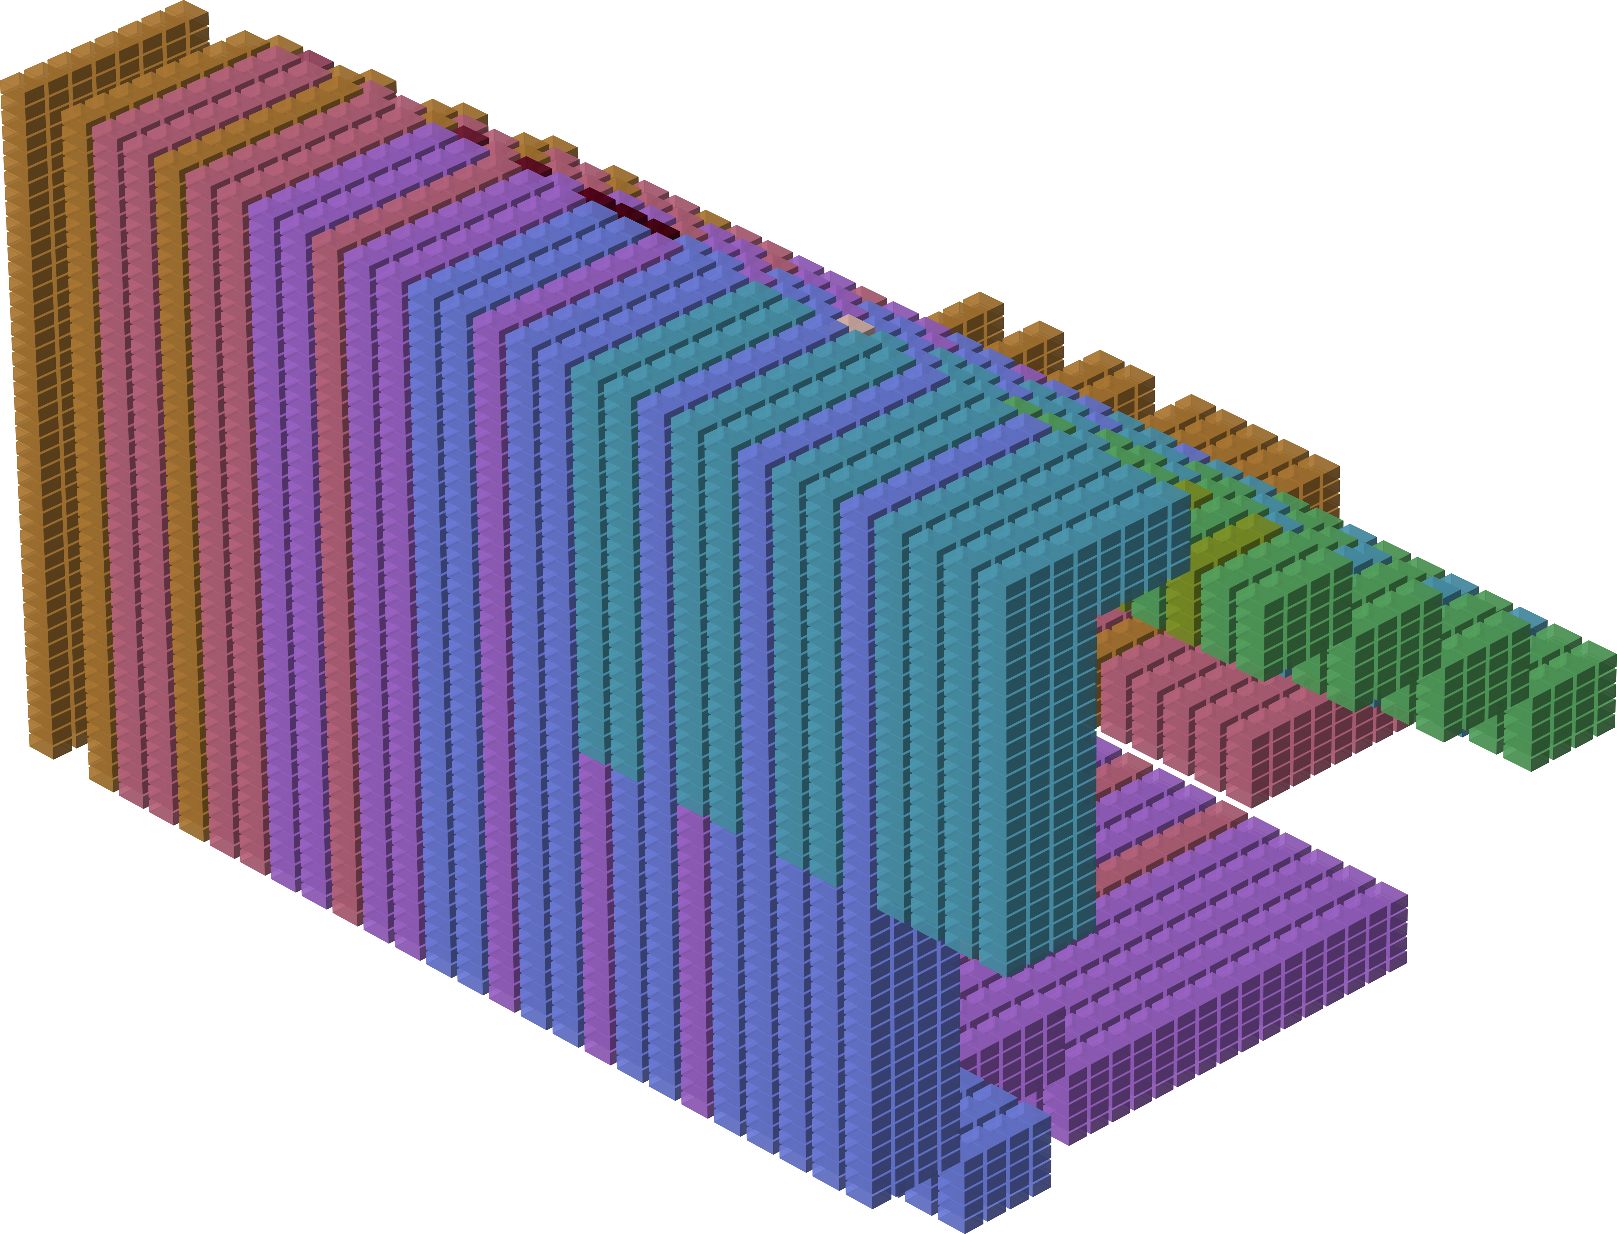
\includegraphics[width=10cm]{src/colorspace_patterns/pattern10-225.png}%
    \end{adjustbox}
\caption{'User LightForm 2'.}
\end{figure}
\end{minipage}
\begin{minipage}[b]{0.48\linewidth}
\vspace{0.5cm}
\begin{lrbox}{\mybox}%
\hspace{1cm}
\begin{lstlisting}[basicstyle=\ttfamily\tiny,escapechar=\%]
userLightform2XPosArray
  .BYTE $FF,$FE,$FD,$55                 ;          22
  .BYTE $01,$02,$02,$02,$02,$02,$55     ;           2
  .BYTE $02,$02,$02,$02,$01,$55         ;        1  2
  .BYTE $00,$FF,$FE,$FD,$FB,$FC,$55     ;       1   2
  .BYTE $FA,$F9,$55                     ;      1    2
  .BYTE $F8,$55                         ;           3
userLightform2YPosArray                 ;           3
  .BYTE $01,$02,$03,$55                 ;           3
  .BYTE $FF,$FF,$00,$01,$02,$03,$55     ;           3
  .BYTE $04,$05,$06,$07,$08,$55         ; 6        3 
  .BYTE $09,$09,$0A,$0A,$0A,$0A,$55     ;  55    44  
  .BYTE $09,$09,$55                     ;    4444    
  .BYTE $08,$55
\end{lstlisting}
\end{lrbox}%
\scalebox{0.8}{\usebox{\mybox}}
\subfile{colorspace_patterns/tables/pattern10.tex}
\end{minipage}
%
%
\begin{minipage}[b]{0.48\linewidth}
\vspace{-1cm}
\begin{figure}[H]
    \centering
    \begin{adjustbox}{width=5cm,margin=0cm 0cm}
      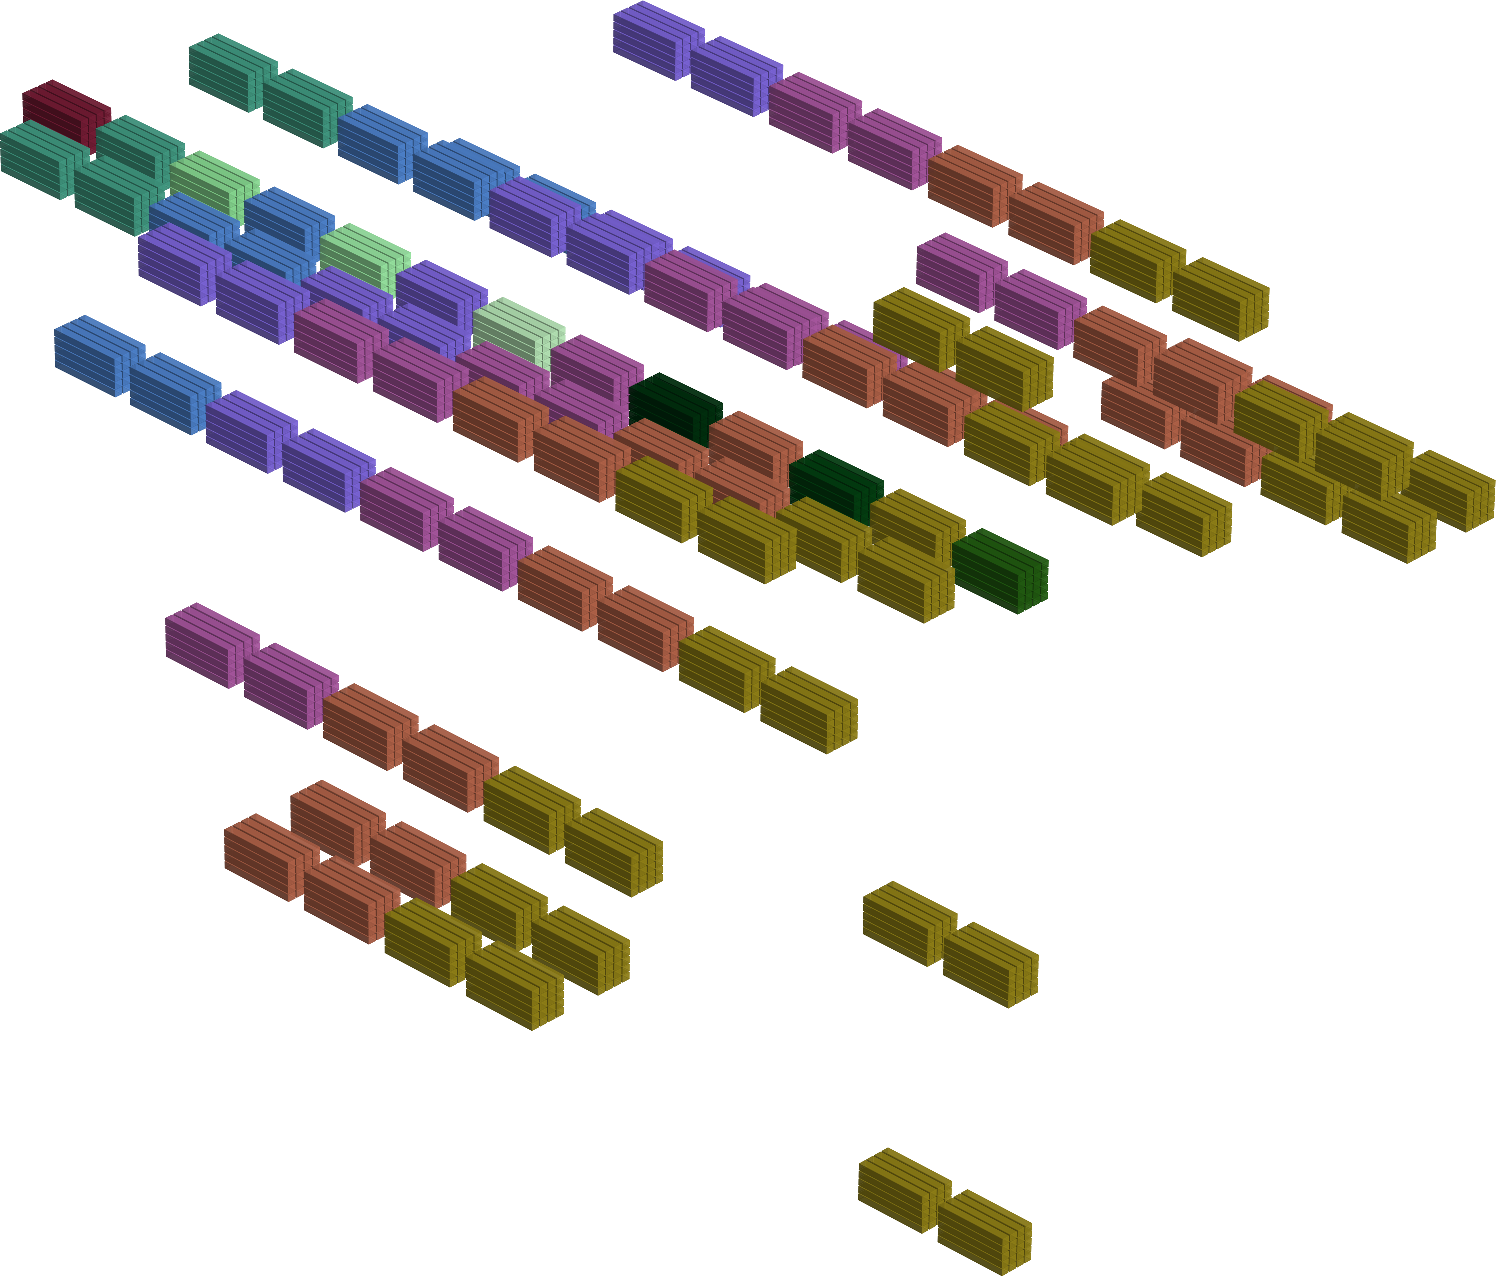
\includegraphics[width=10cm]{src/colorspace_patterns/pattern11-45.png}%
    \end{adjustbox}
    \begin{adjustbox}{width=5cm,margin=0cm 0cm}
      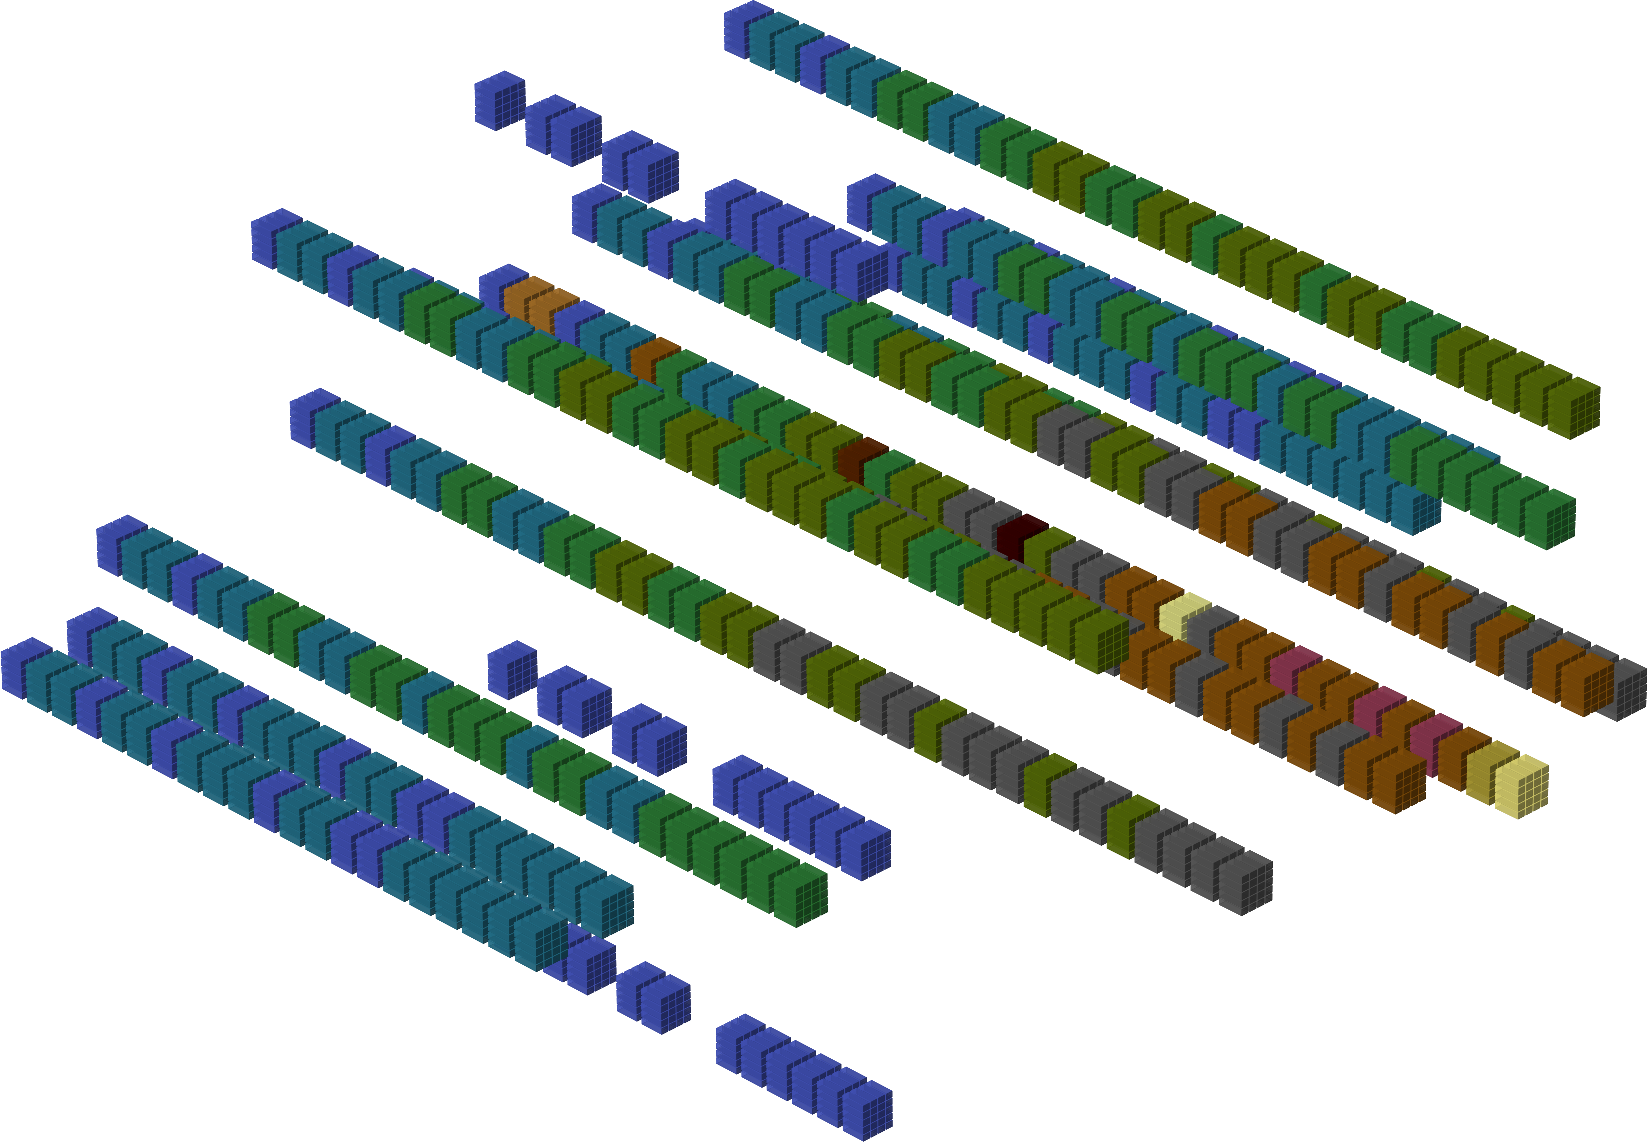
\includegraphics[width=10cm]{src/colorspace_patterns/pattern11-225.png}%
    \end{adjustbox}
\caption{'User LightForm 3'.}
\end{figure}
\end{minipage}
\begin{minipage}[b]{0.48\linewidth}
\vspace{-0.3cm}
\begin{lrbox}{\mybox}%
\hspace{0.5cm}
\begin{lstlisting}[basicstyle=\ttfamily\tiny,escapechar=\%]
userLightform3XPosArray
.BYTE $FD,$03,$55         ;                6               
.BYTE $FA,$06,$55         ;        3              3        
.BYTE $F8,$07,$55         ;                                
.BYTE $F4,$0C,$55         ;                                
.BYTE $F3,$F1,$0D,$0F,$55 ;             1     1            
.BYTE $00,$00,$00,$55     ;                                
.BYTE $55                 ;          2           2         
userLightform3YPosArray   ;    4                       4   
.BYTE $FF,$FF,$55         ;                                
.BYTE $01,$01,$55         ; 5 5                         5 5
.BYTE $FC,$FC,$55         ;                                
.BYTE $02,$02,$55         ;                                
.BYTE $04,$04,$04,$04,$55 ;                                
.BYTE $FB,$0A,$11,$55     ;                                
.BYTE $55                 ;                                
                          ;                6               
                          ;                                
                          ;                                
                          ;                                
                          ;                                
                          ;                                
                          ;                                
                          ;                6               
\end{lstlisting}
\end{lrbox}%
\scalebox{0.8}{\usebox{\mybox}}
\subfile{colorspace_patterns/tables/pattern11.tex}
\end{minipage}
%
%
\begin{minipage}[b]{0.48\linewidth}
\vspace{1cm}
\begin{figure}[H]
    \centering
    \begin{adjustbox}{width=5cm,margin=0cm 0cm}
      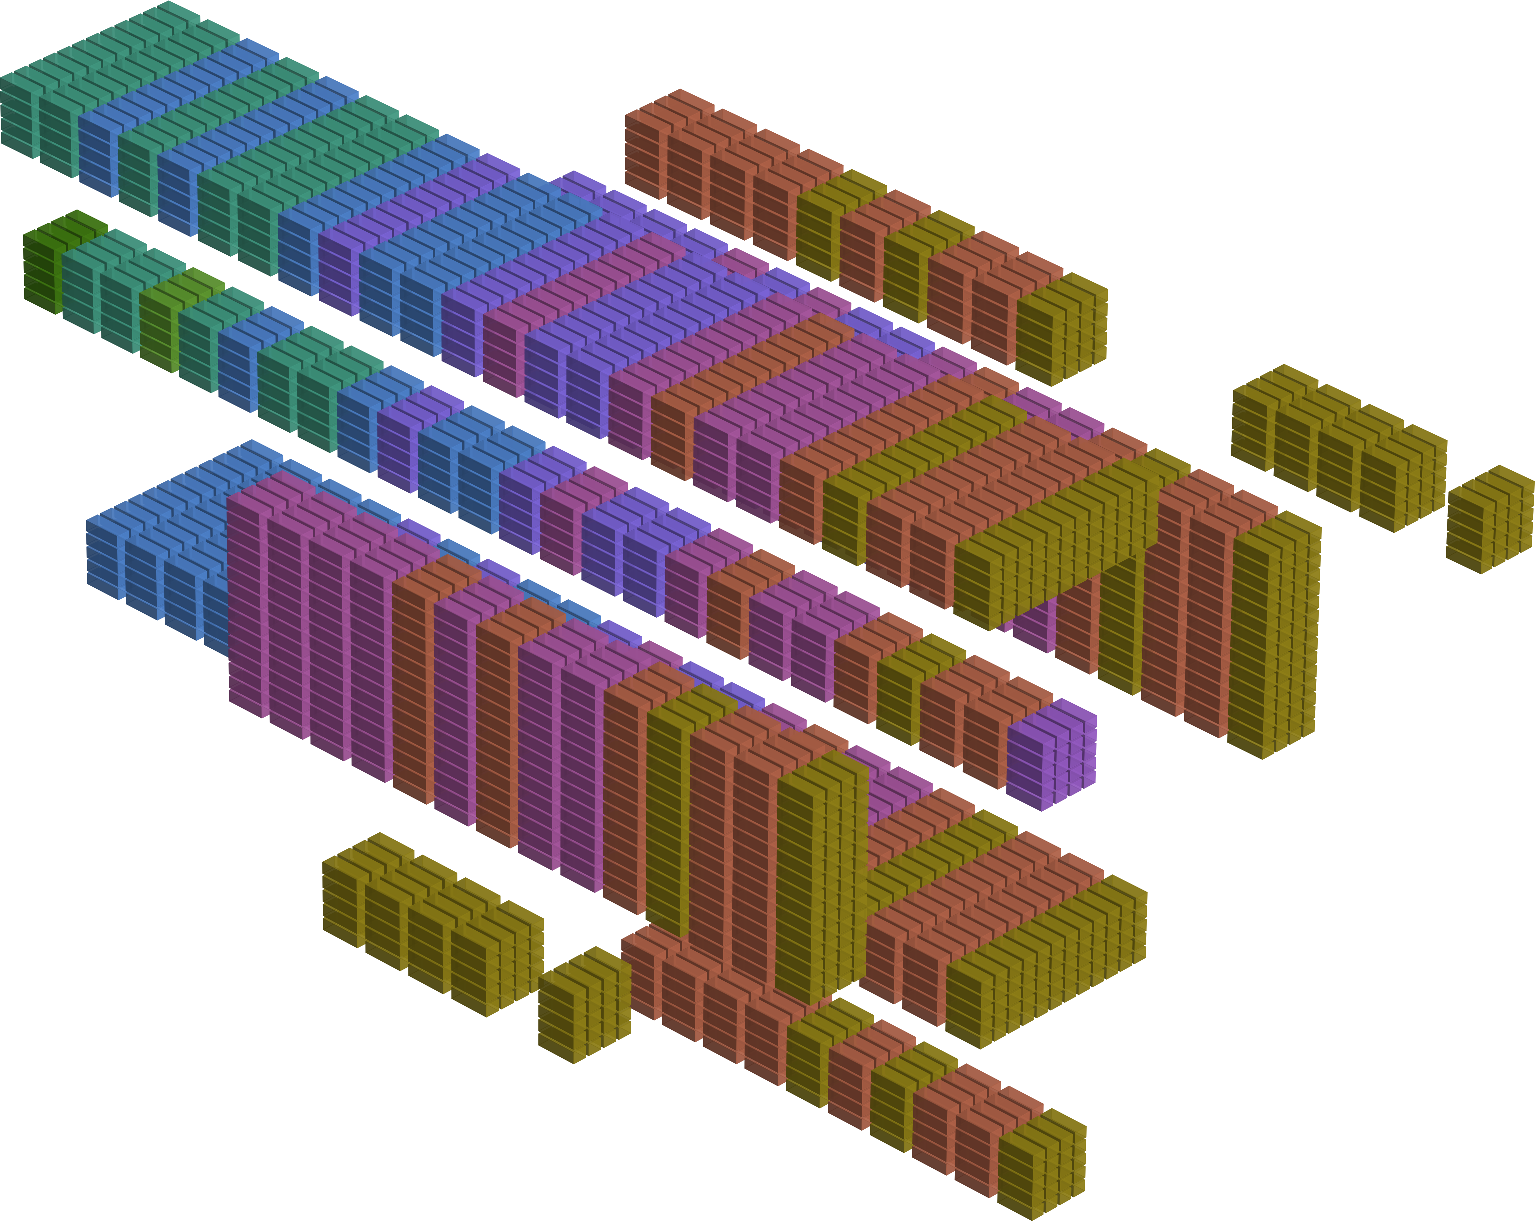
\includegraphics[width=10cm]{src/colorspace_patterns/pattern12-45.png}%
    \end{adjustbox}
    \begin{adjustbox}{width=5cm,margin=0cm 0cm}
      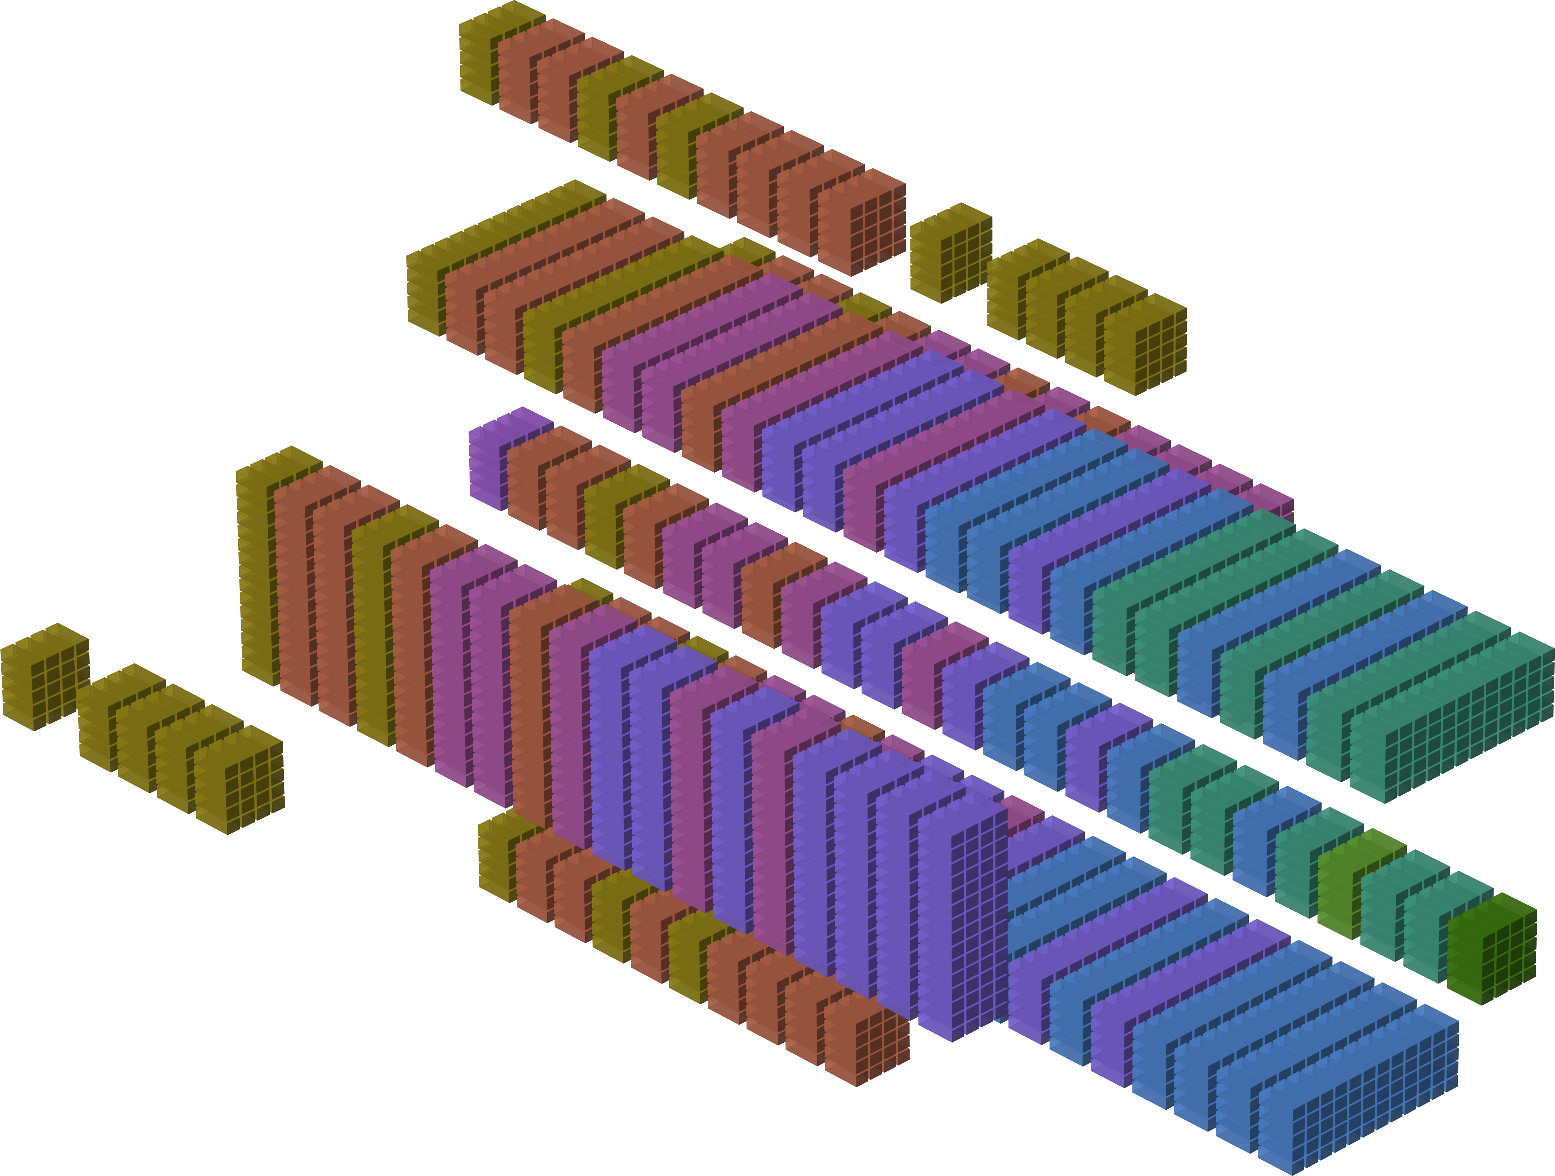
\includegraphics[width=10cm]{src/colorspace_patterns/pattern12-225.png}%
    \end{adjustbox}
\caption{'User LightForm 4'.}
\end{figure}
\end{minipage}
\begin{minipage}[b]{0.48\linewidth}
\vspace{1cm}
\begin{lrbox}{\mybox}%
\hspace{1cm}
\begin{lstlisting}[basicstyle=\ttfamily\tiny,escapechar=\%]
userLightform4XPosArray
        .BYTE $FF,$00,$01,$55 ;         5        
        .BYTE $FF,$00,$01,$55 ;                  
        .BYTE $04,$04,$04,$55 ;                  
        .BYTE $FC,$FC,$FC,$55 ;        111       
        .BYTE $00,$00,$55     ;                  
        .BYTE $F8,$08,$55     ;     4       3    
userLightform4YPosArray       ; 6   4       3   6
        .BYTE $FD,$FD,$FD,$55 ;     4       3    
        .BYTE $03,$03,$03,$55 ;                  
        .BYTE $FF,$00,$01,$55 ;        222       
        .BYTE $FF,$00,$01,$55 ;                  
        .BYTE $FA,$06,$55     ;                  
        .BYTE $00,$00,$55     ;         5        
\end{lstlisting}
\end{lrbox}%
\scalebox{0.8}{\usebox{\mybox}}
\subfile{colorspace_patterns/tables/pattern12.tex}
\end{minipage}
%
\begin{figure}[H]
    \centering
    \begin{adjustbox}{width=13cm,center}
      \frame{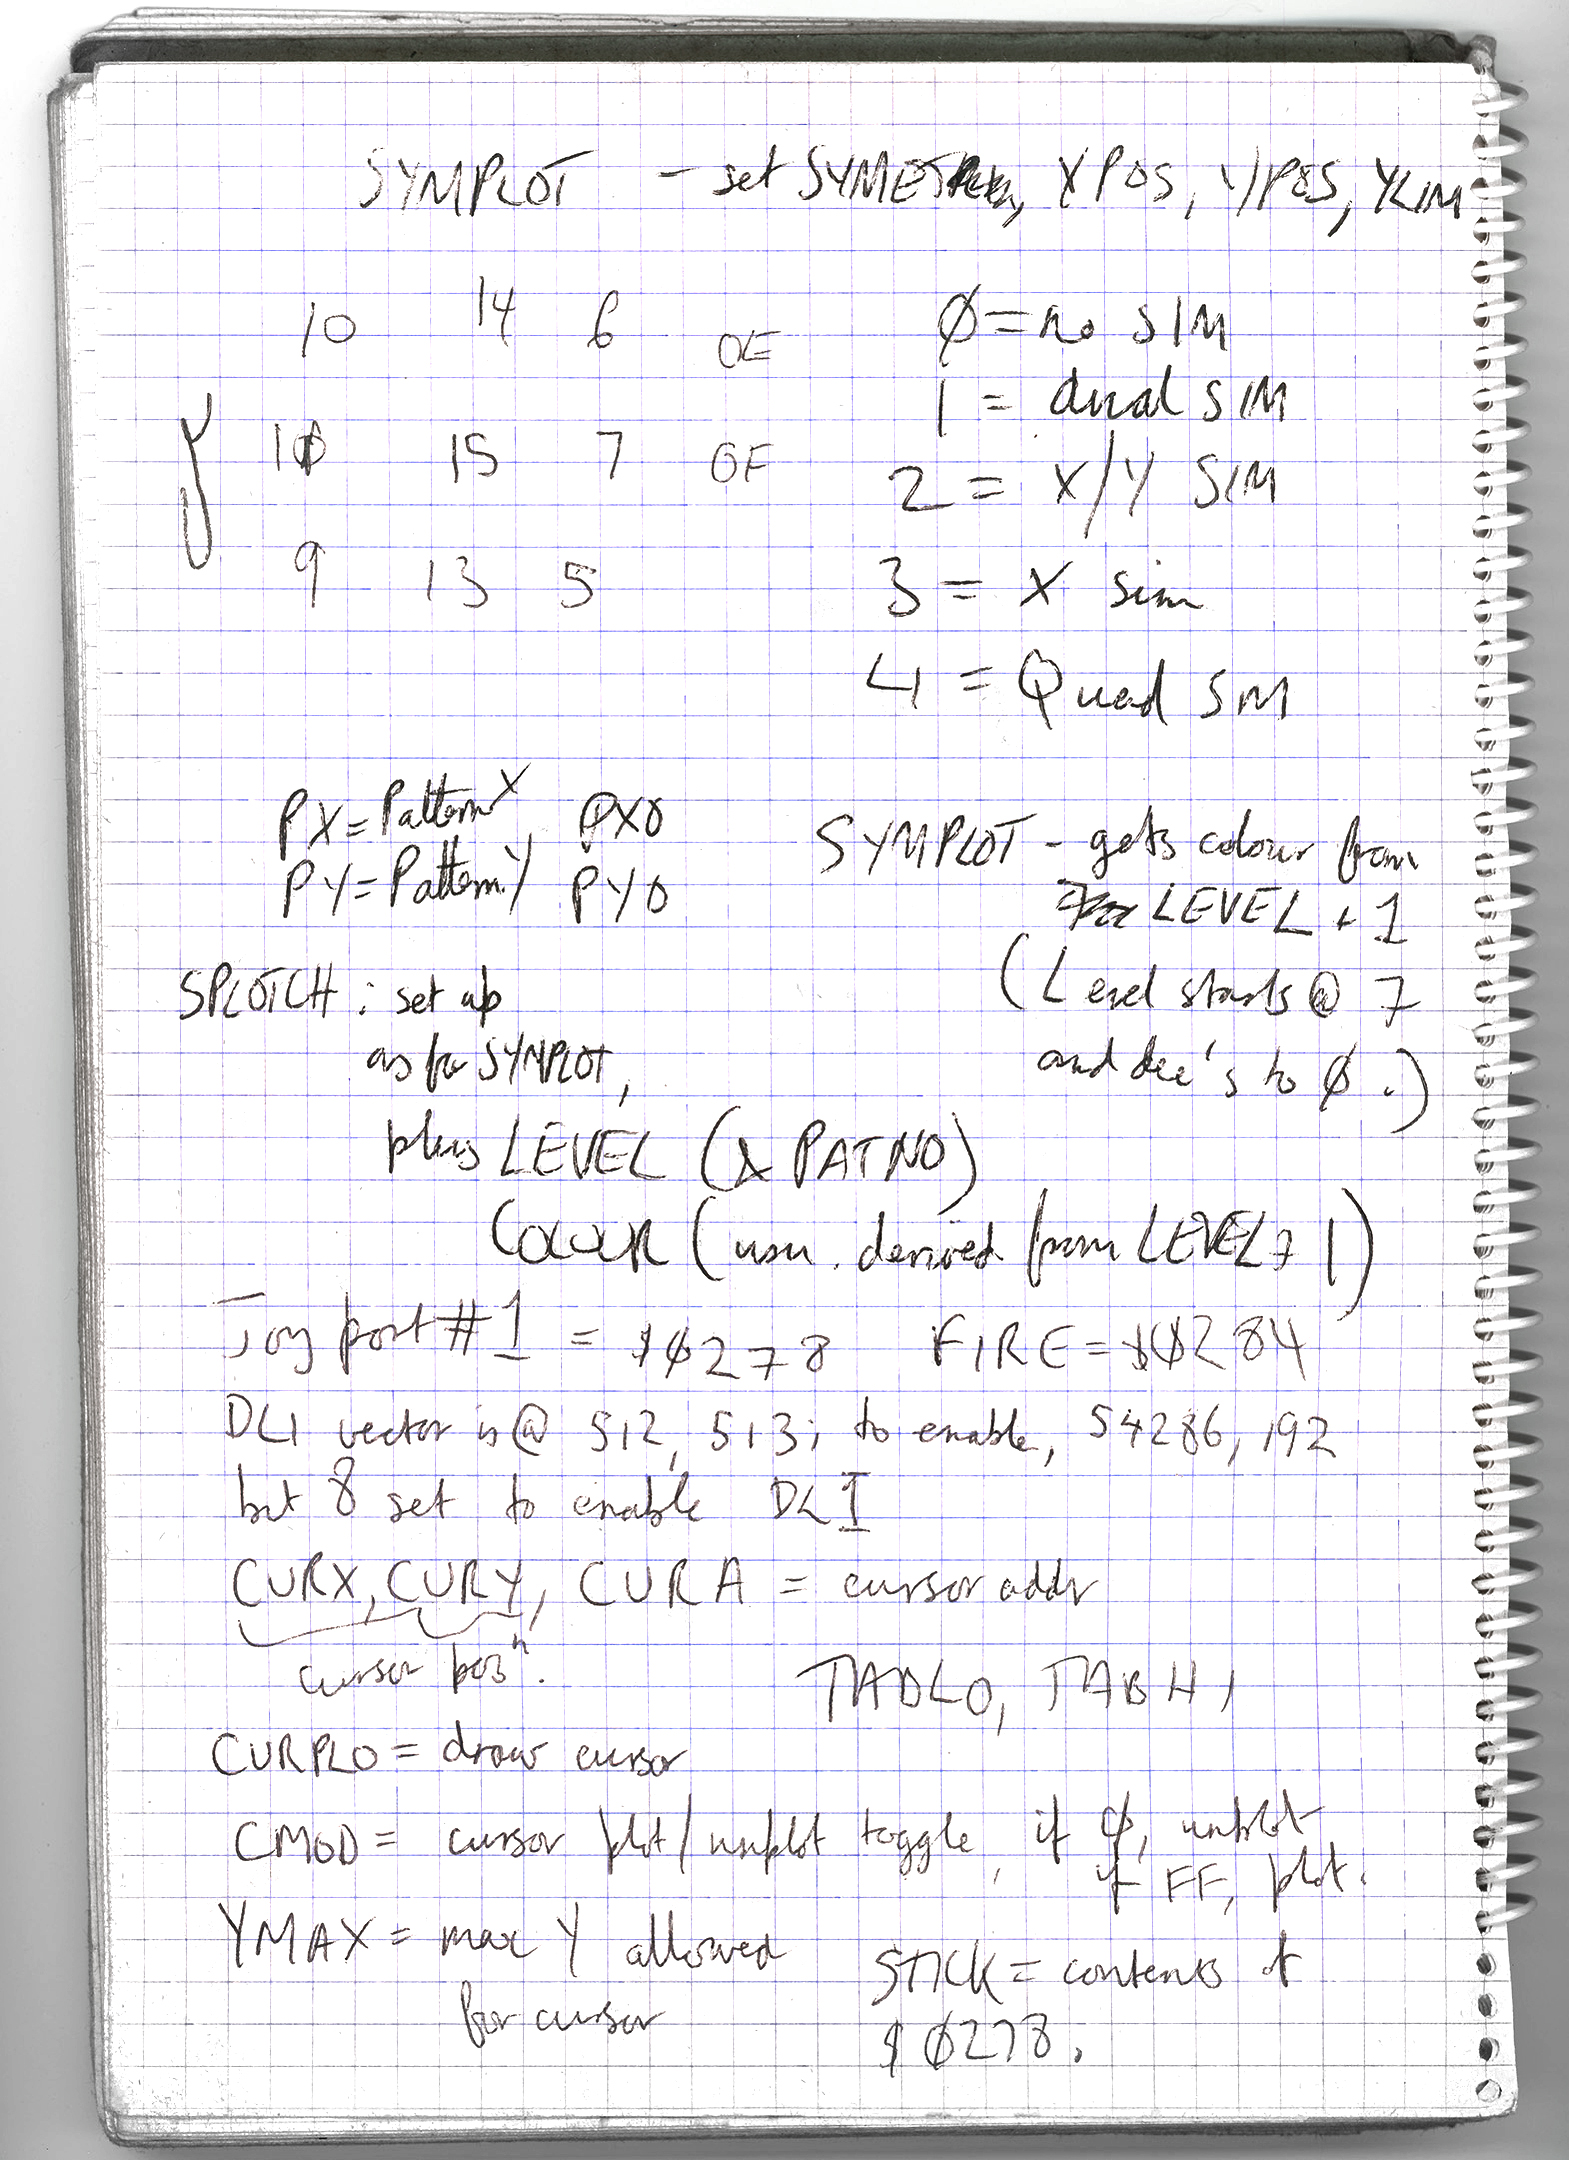
\includegraphics[width=13cm]{src/patterns/lightsynth_01.jpg}}%
    \end{adjustbox}
\caption{From Jeff Minter's development notebook for Colourspace}
\end{figure}
\clearpage
At first glance this notebook could be for Psychedelia as much as for Colourspace. However there is a tell-tale reference
to 'dlists', i.e. 'display lists', which are a feature of the Atari 800 architecture rather than the Commodore series of 
computers.

\textbf{First Half. \icode{\textbf{SYMPLOT}}:} 
The first half of this excerpt from from Jeff Minter's development notes sketch out some initial details on the routine
we call \icode{PaintPixelForCurrentSymmetry}, and which he calls \icode{SYMPLOT} (i.e. 'symmetry plot'). As he says, the
purpose of the routine is to 'set symm[etry' using the \icode{XPOS} (\icode{pixelXPosition}) and \icode{YPOS} (\icode{pixelYPosition}).

The final routine makes no use of a \icode{YLIM} variable, instead it looks at \icode{\#NUM\_ROWS} as a constant value to determine the
bottom of the screen. The extract also notes that \icode{SYMPLOT} gets its 'colour from LEVEL + 1 (Level starts @ 7 and dec's to 0)'.
This is the mechanic we described in detail in \hyperref[sec:listing_pattern]{\textcolor{blue}{'soul of a light machine'}}.

\clearpage

%
\begin{minipage}[b]{0.48\linewidth}
\begin{figure}[H]
    \centering
    \begin{adjustbox}{width=5cm,margin=0cm 0cm}
      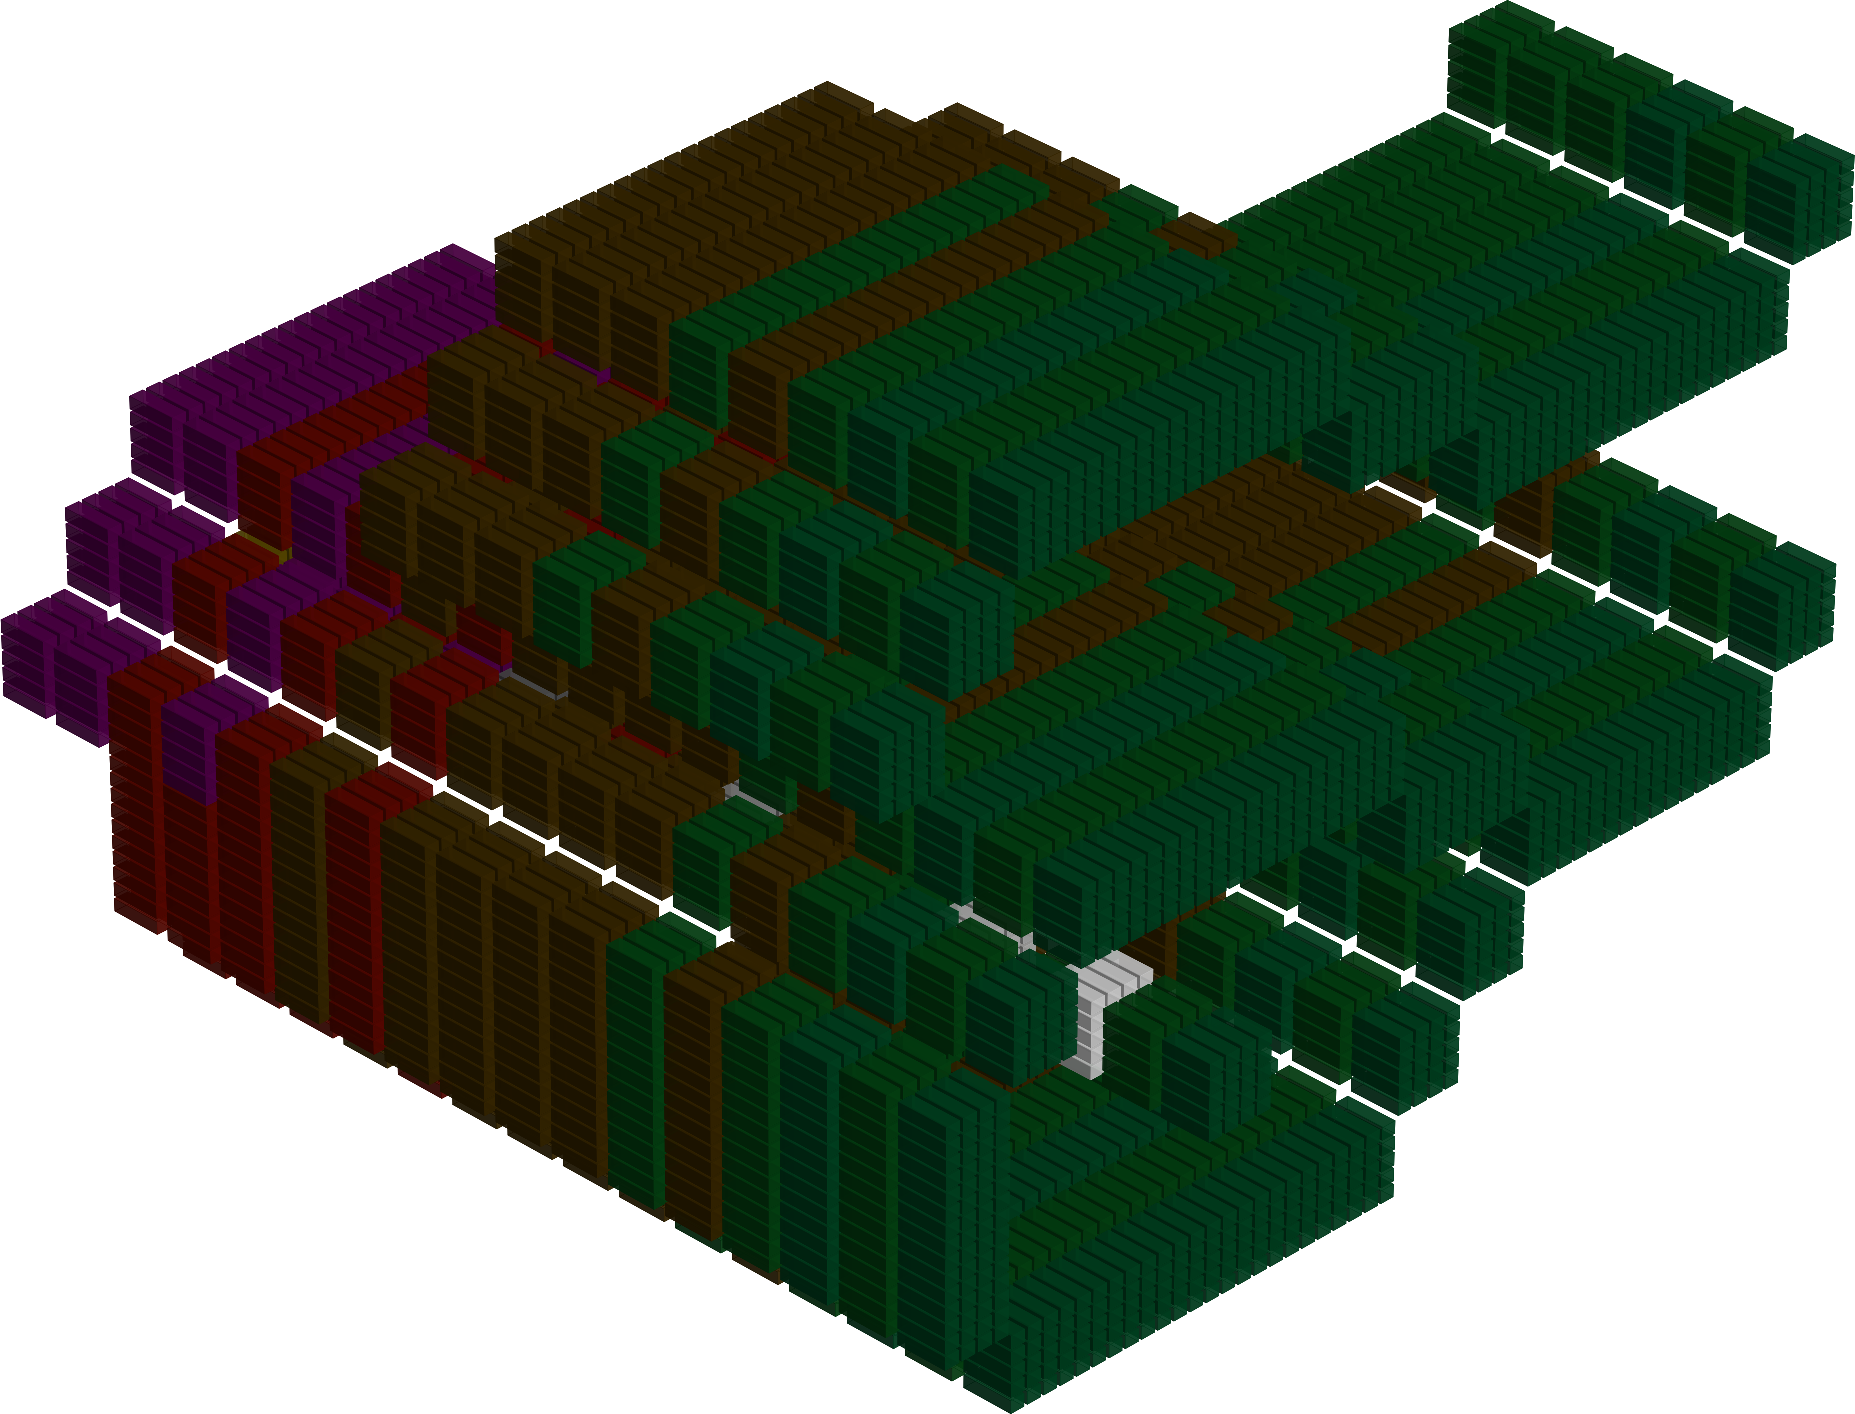
\includegraphics[width=10cm]{src/colorspace_patterns/pattern13-45.png}%
    \end{adjustbox}
    \begin{adjustbox}{width=5cm,margin=0cm 0cm}
      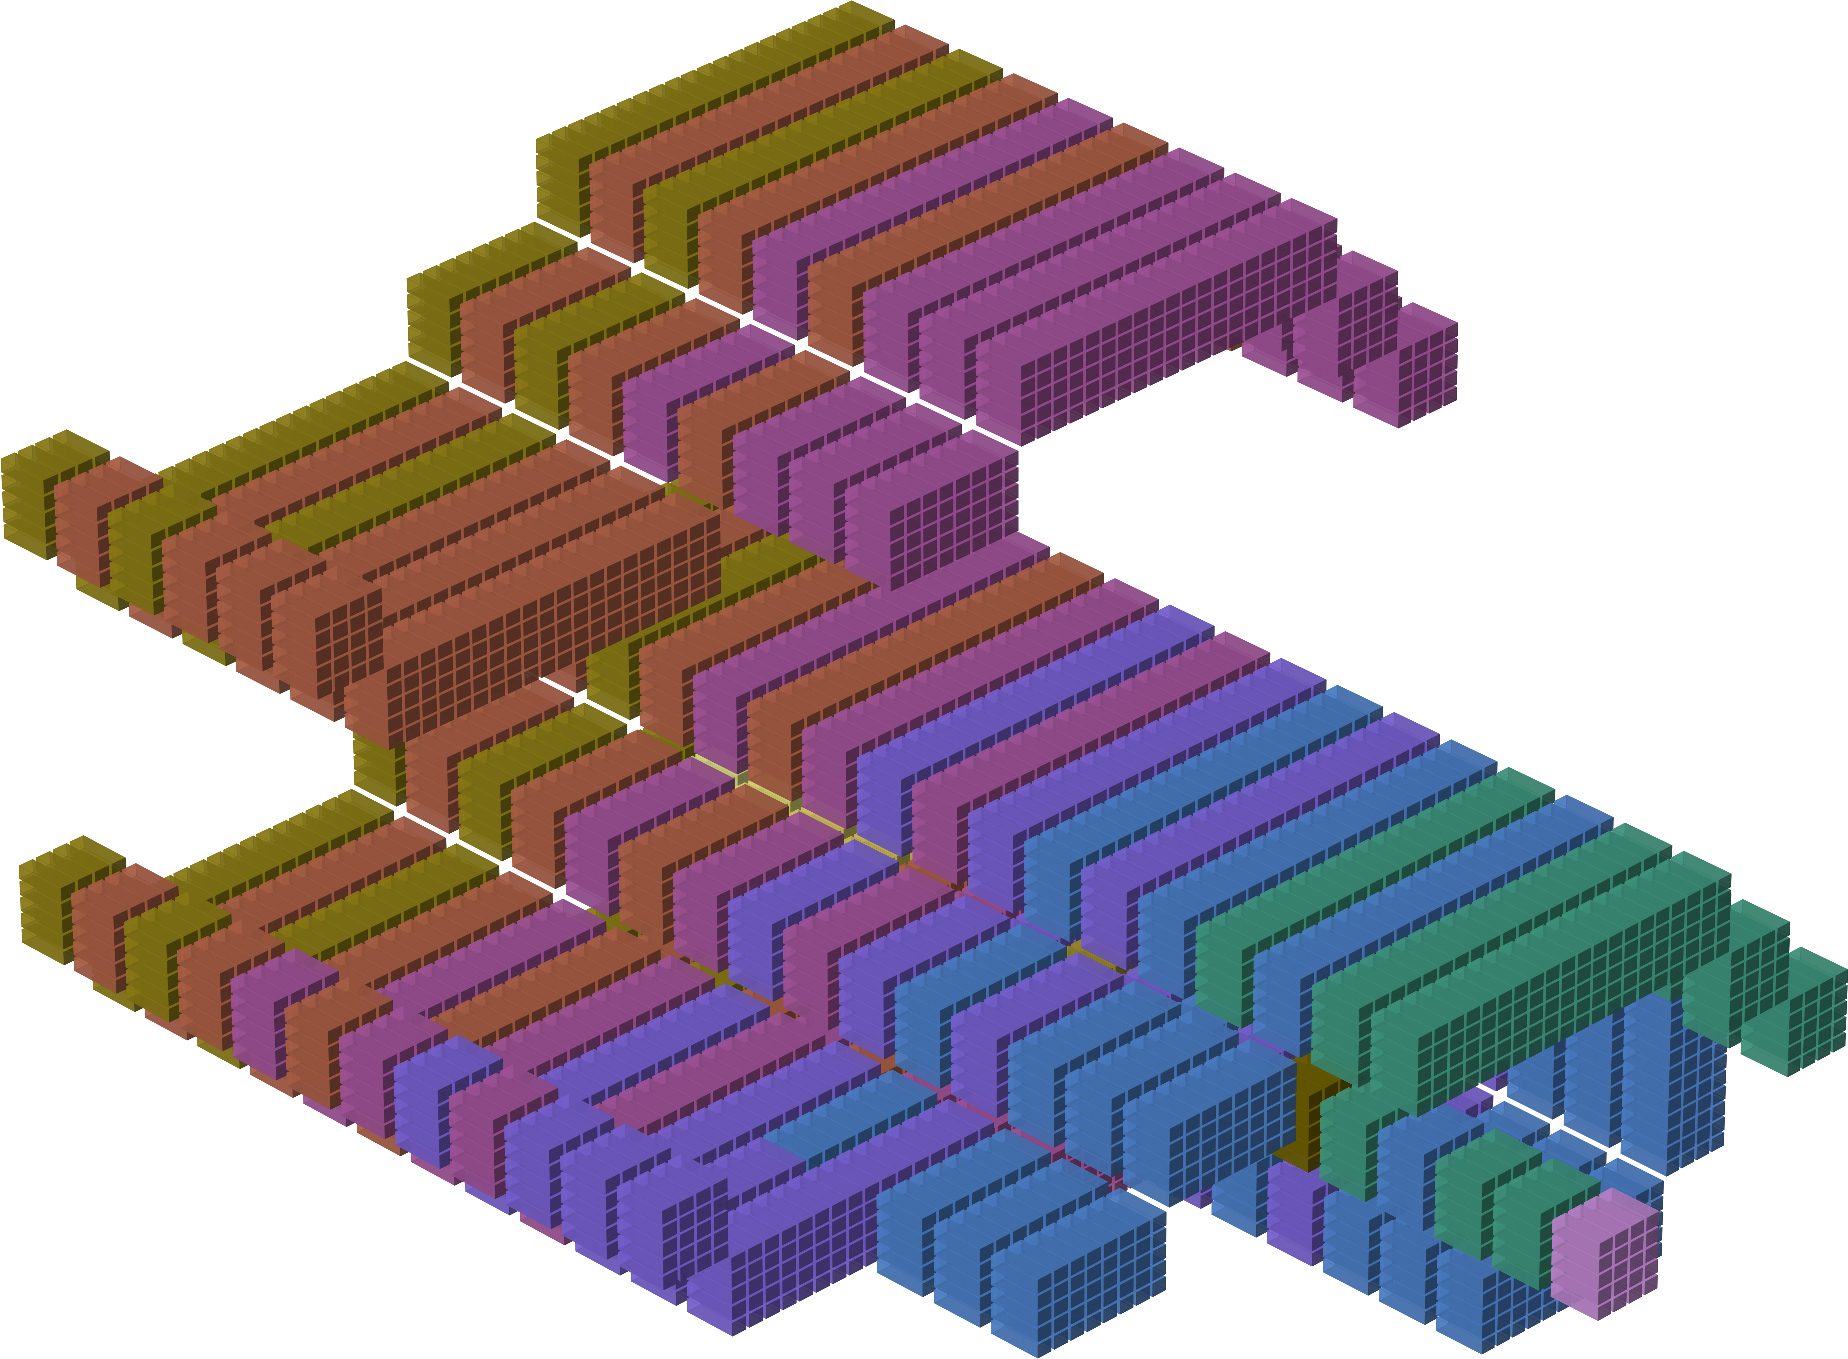
\includegraphics[width=10cm]{src/colorspace_patterns/pattern13-225.png}%
    \end{adjustbox}
\caption{'User LightForm 5'.}
\end{figure}
\end{minipage}
\begin{minipage}[b]{0.68\linewidth}
\begin{lrbox}{\mybox}%
\hspace{1cm}
\begin{lstlisting}[basicstyle=\ttfamily\tiny,escapechar=\%]
userLightform5XPosArray
  .BYTE $FE,$FF,$00,$01,$02,$FD,$FC,$55                      ;   44444        
  .BYTE $03,$04,$05,$06,$FC,$FC,$FD,$FF,$FE,$55              ;  4     44     5
  .BYTE $07,$08,$09,$04,$03,$55                              ; 4        55555 
  .BYTE $00,$01,$02,$FB,$FC,$FD,$FE,$FF,$00,$01,$02,$03,$55  ;                
  .BYTE $04,$05,$06,$07,$08,$09,$55                          ;                
  .BYTE $00,$55                                              ;    11111       
userLightform5YPosArray                                      ;   1     22    3
  .BYTE $FD,$FD,$FD,$FD,$FD,$FE,$FF,$55                      ;  1        2233 
  .BYTE $FE,$FE,$FF,$FF,$00,$01,$02,$02,$02,$55              ;  2   6   3     
  .BYTE $FF,$FF,$FE,$00,$01,$55                              ;  2      3      
  .BYTE $02,$02,$02,$FA,$F9,$F8,$F8,$F8,$F8,$F8,$F9,$F9,$55  ;   222444       
  .BYTE $FA,$FA,$FA,$FA,$FA,$F9,$55
  .BYTE $00,$55
\end{lstlisting}
\end{lrbox}%
\scalebox{0.8}{\usebox{\mybox}}
\subfile{colorspace_patterns/tables/pattern13.tex}
\end{minipage}
%
%
\begin{minipage}[b]{0.48\linewidth}
\vspace{1cm}
\begin{figure}[H]
    \centering
    \begin{adjustbox}{width=5cm,margin=0cm 0cm}
      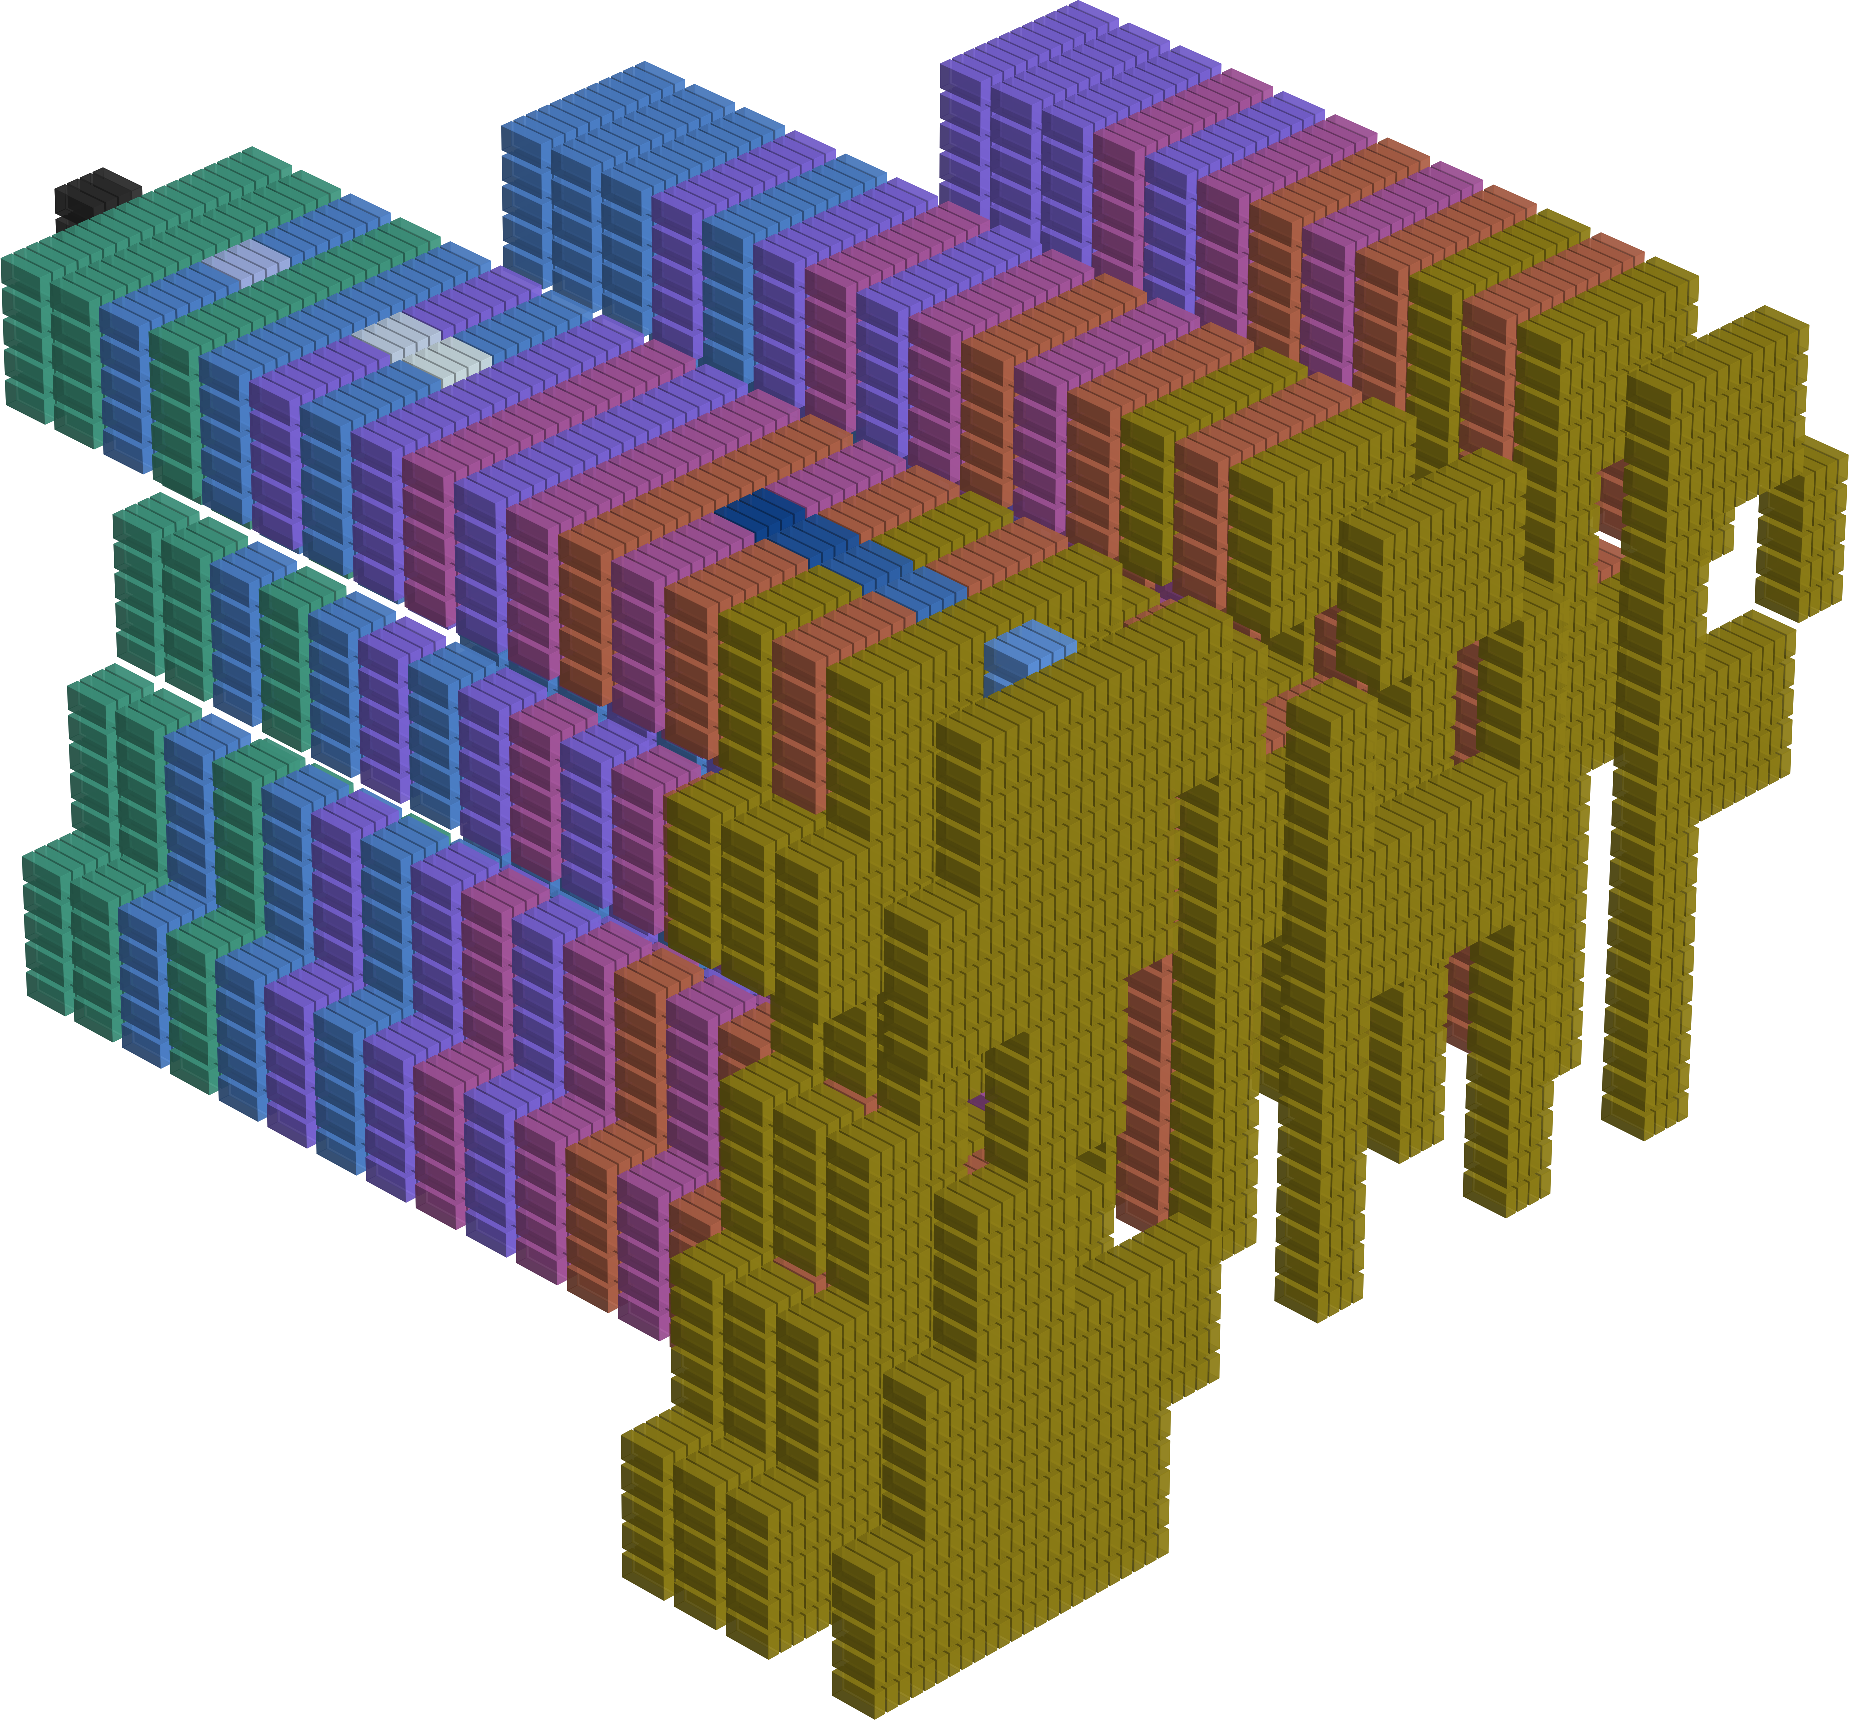
\includegraphics[width=10cm]{src/colorspace_patterns/pattern14-45.png}%
    \end{adjustbox}
    \begin{adjustbox}{width=5cm,margin=0cm 0cm}
      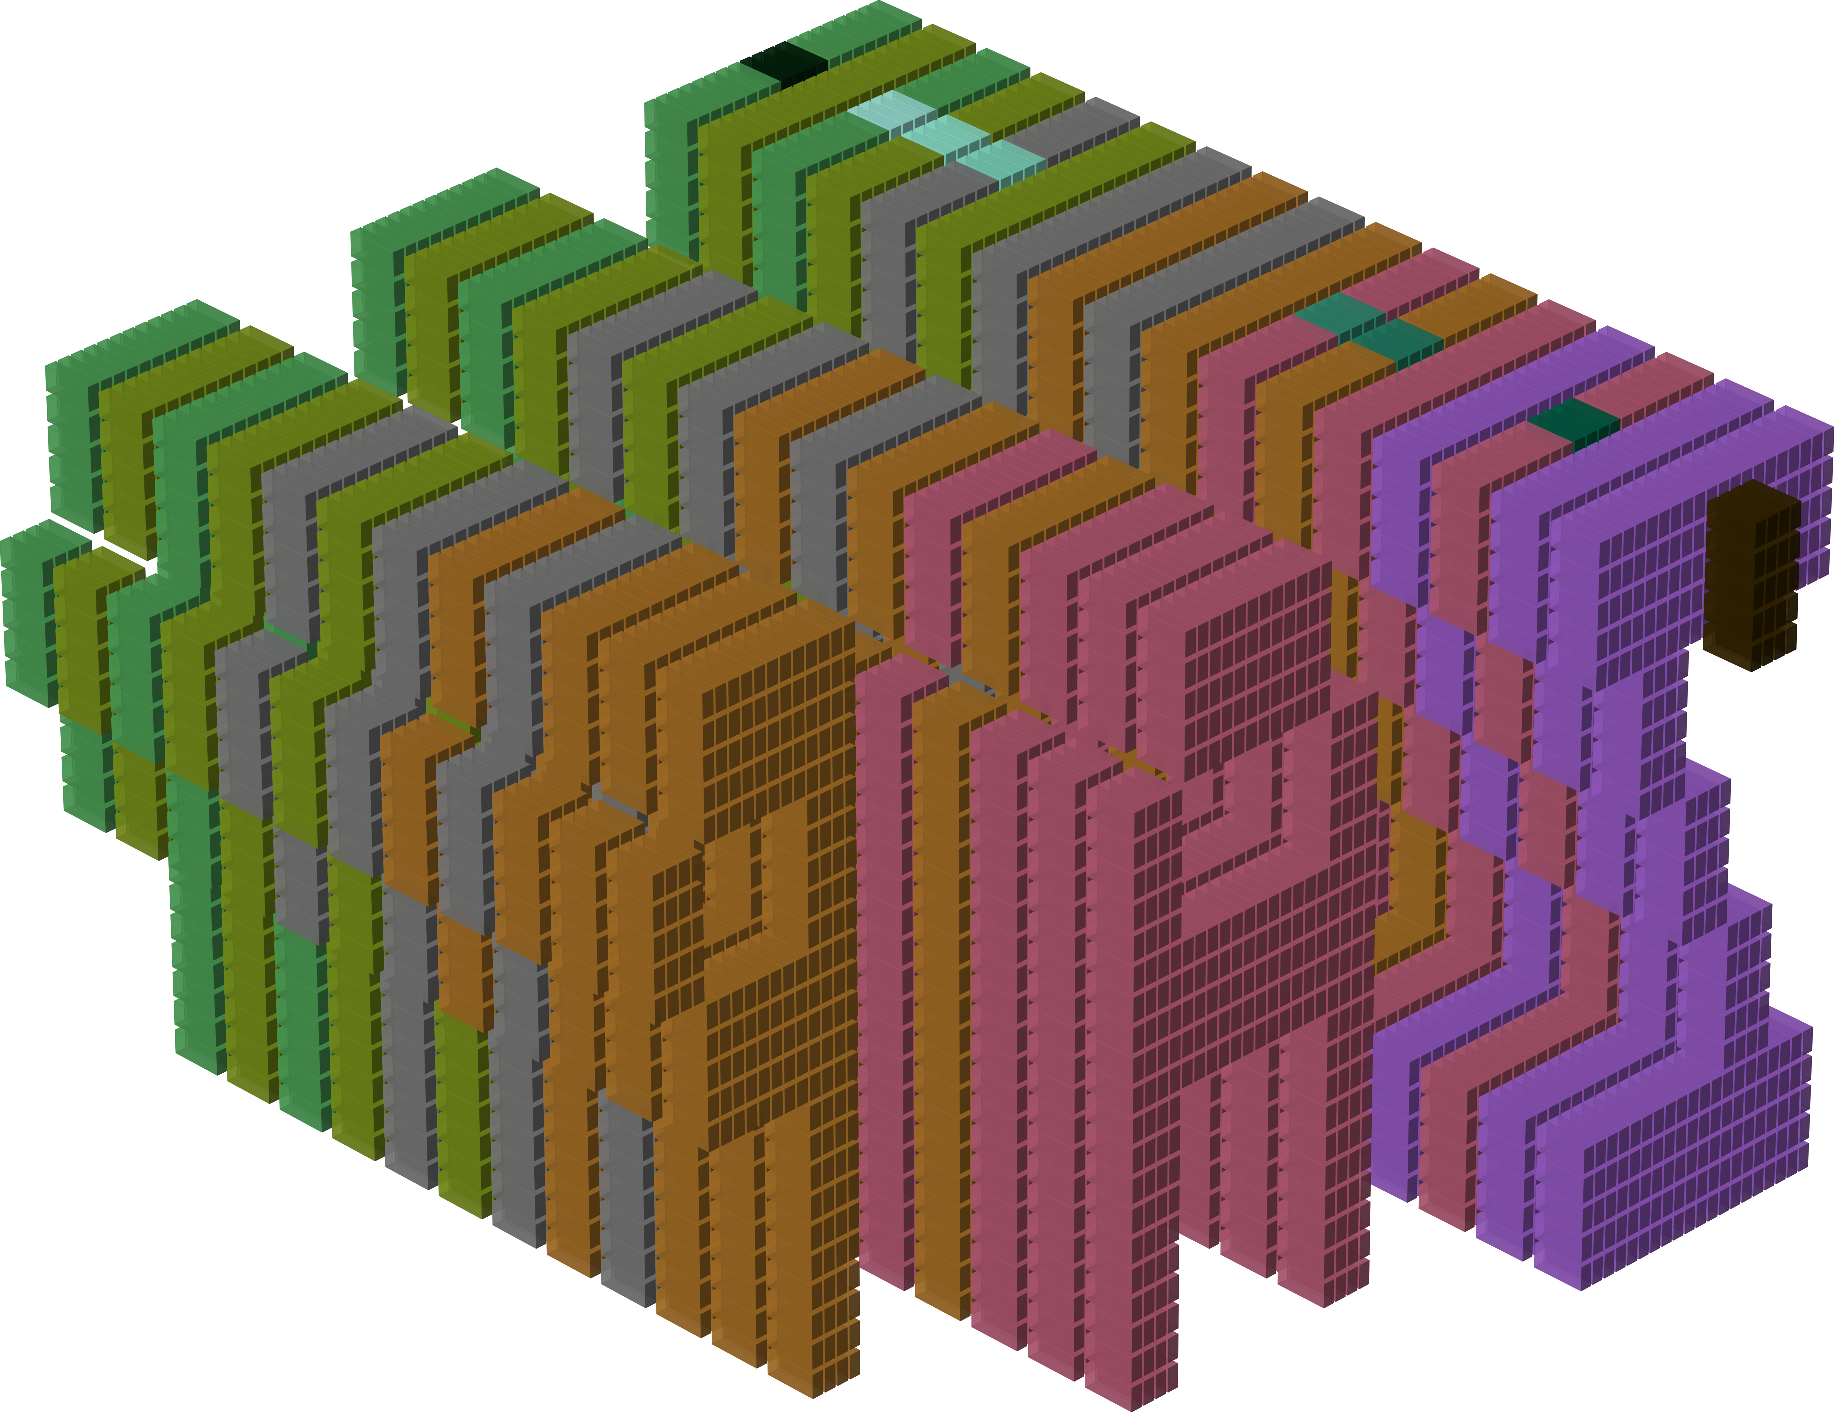
\includegraphics[width=10cm]{src/colorspace_patterns/pattern14-225.png}%
    \end{adjustbox}
\caption{'User LightForm 6'.}
\end{figure}
\end{minipage}
\begin{minipage}[b]{0.68\linewidth}
\vspace{1cm}
\begin{lrbox}{\mybox}%
\hspace{1cm}
\begin{lstlisting}[basicstyle=\ttfamily\tiny,escapechar=\%]
userLightform6XPosArray
  .BYTE $FF,$FE,$01,$02,$01,$00,$FF,$FE
        $FF,$00,$01,$02,$55                ;   11 11   222   333 
  .BYTE $05,$05,$05,$05,$06,$07,$08,$09    ;  66661   2   2  3  3
        $09,$09,$09,$06,$07,$08,$55        ;    61    22222  333 
  .BYTE $0C,$0C,$0C,$0C,$0C,$0D,$0E,$0F    ;   61     2   2  3   
        $0D,$0E,$55                        ;  611111  2   2  3    
  .BYTE $55                                ; 666666              
  .BYTE $55                                                         
  .BYTE $FD,$FE,$FF,$00,$FF,$FE,$FD,$FC
        $FD,$FE,$FF,$00,$01,$55     
userLightform6YPosArray
  .BYTE $00,$00,$00,$00,$01,$02,$03,$04
        $04,$04,$04,$04,$55
  .BYTE $04,$03,$02,$01,$00,$00,$00,$01
        $02,$03,$04,$02,$02,$02,$55
  .BYTE $04,$03,$02,$00,$01,$00,$00,$01
        $02,$02,$55
  .BYTE $55
  .BYTE $55
  .BYTE $01,$01,$01,$01,$02,$03,$04,$05
        $05,$05,$05,$05,$05,$55
\end{lstlisting}
\end{lrbox}%
\scalebox{0.8}{\usebox{\mybox}}
\subfile{colorspace_patterns/tables/pattern14.tex}
\end{minipage}
%
%
\begin{minipage}[b]{0.48\linewidth}
\begin{figure}[H]
    \centering
    \begin{adjustbox}{width=5cm,margin=0cm -1cm}
      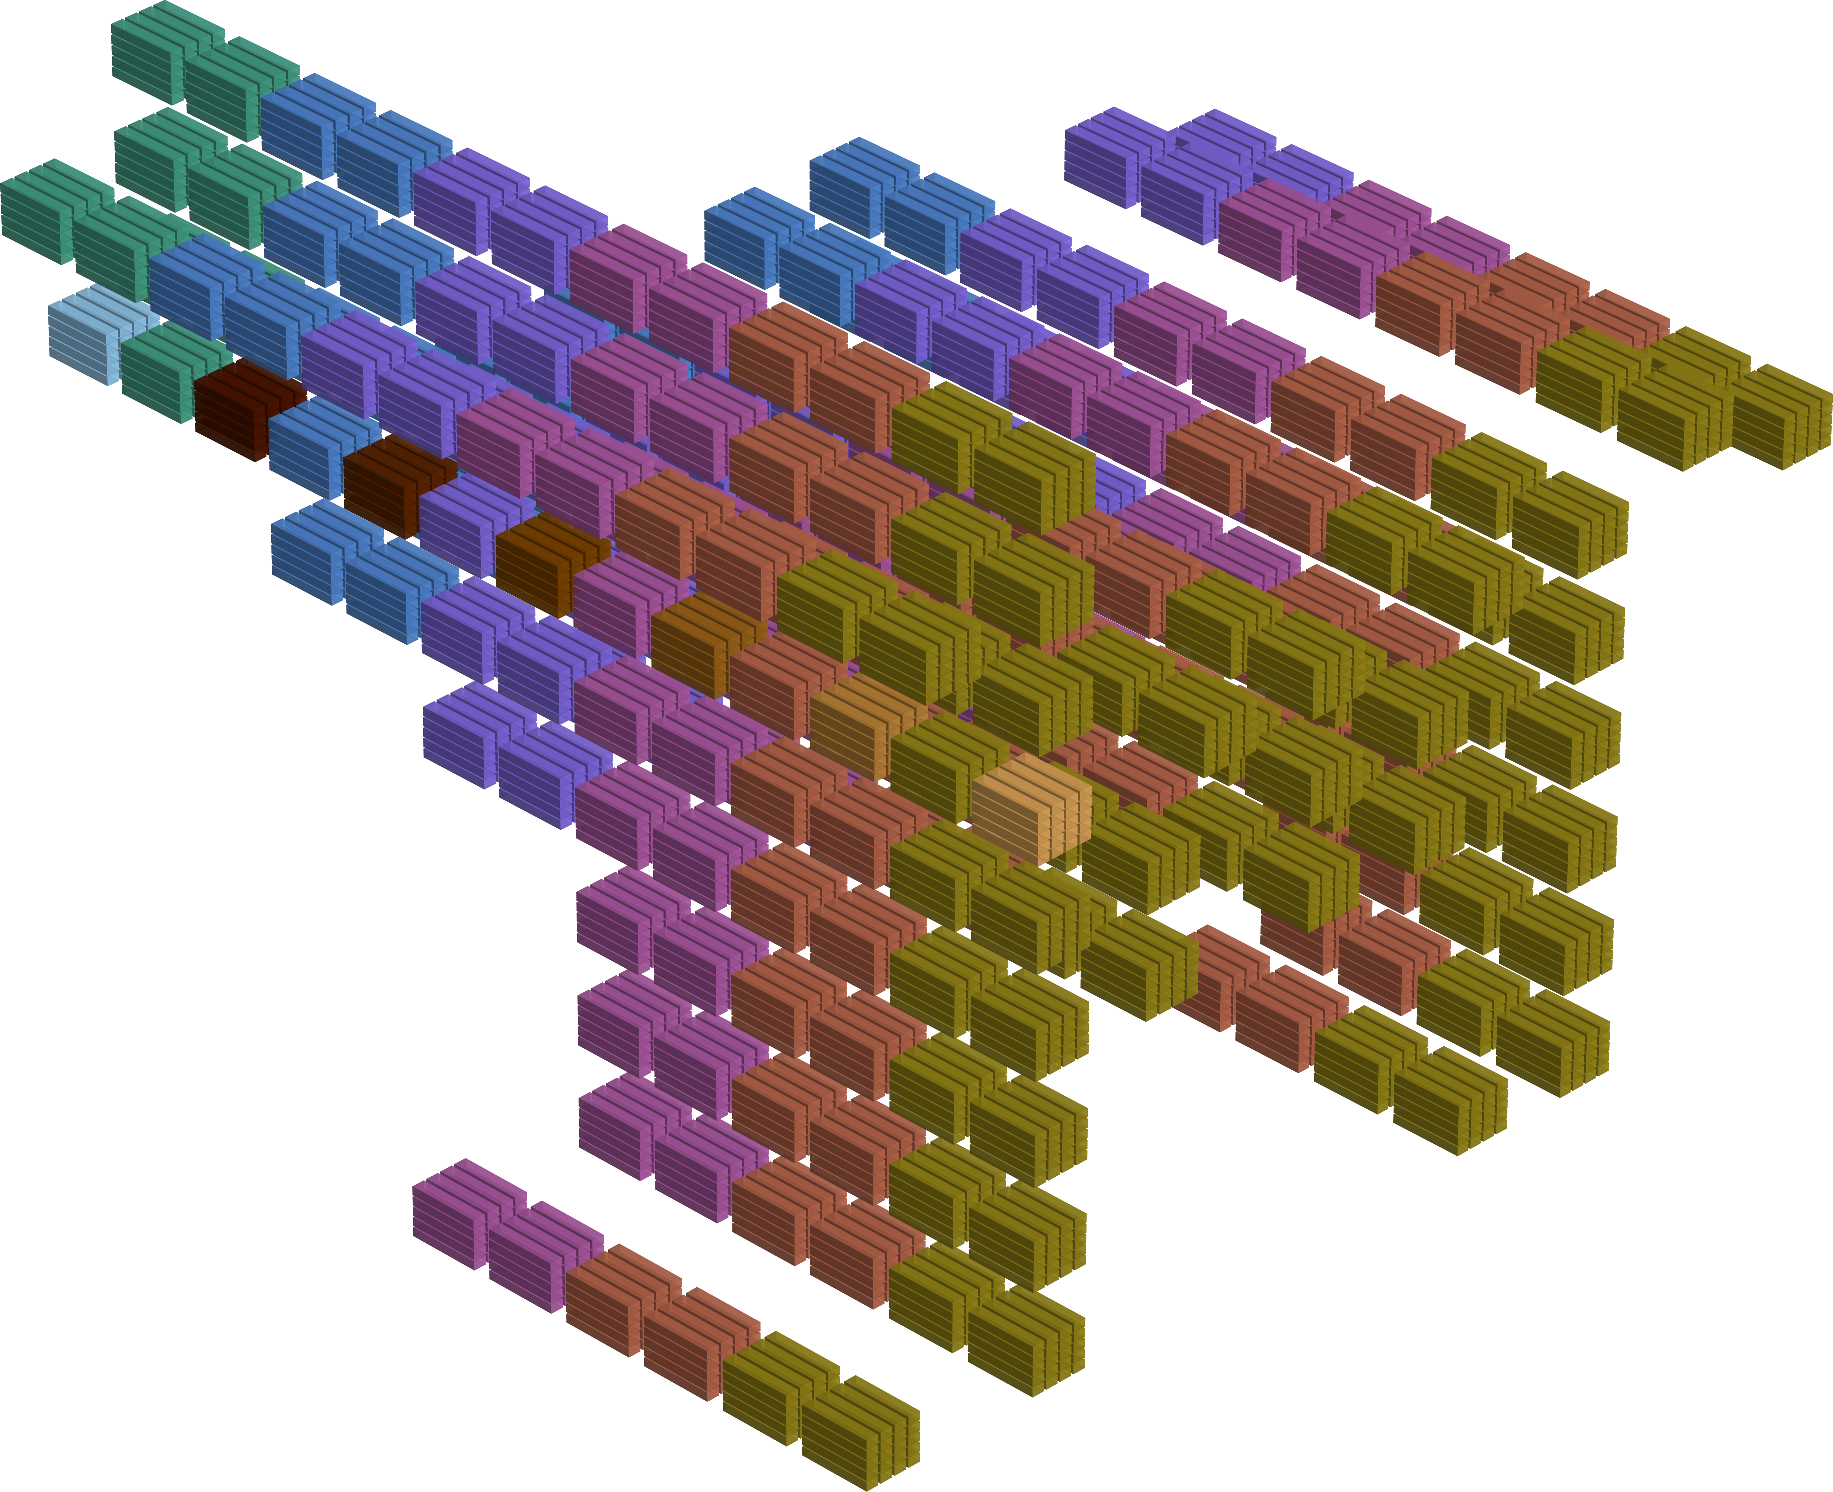
\includegraphics[width=10cm]{src/colorspace_patterns/pattern15-45.png}%
    \end{adjustbox}
    \begin{adjustbox}{width=5cm,margin=0cm 0cm}
      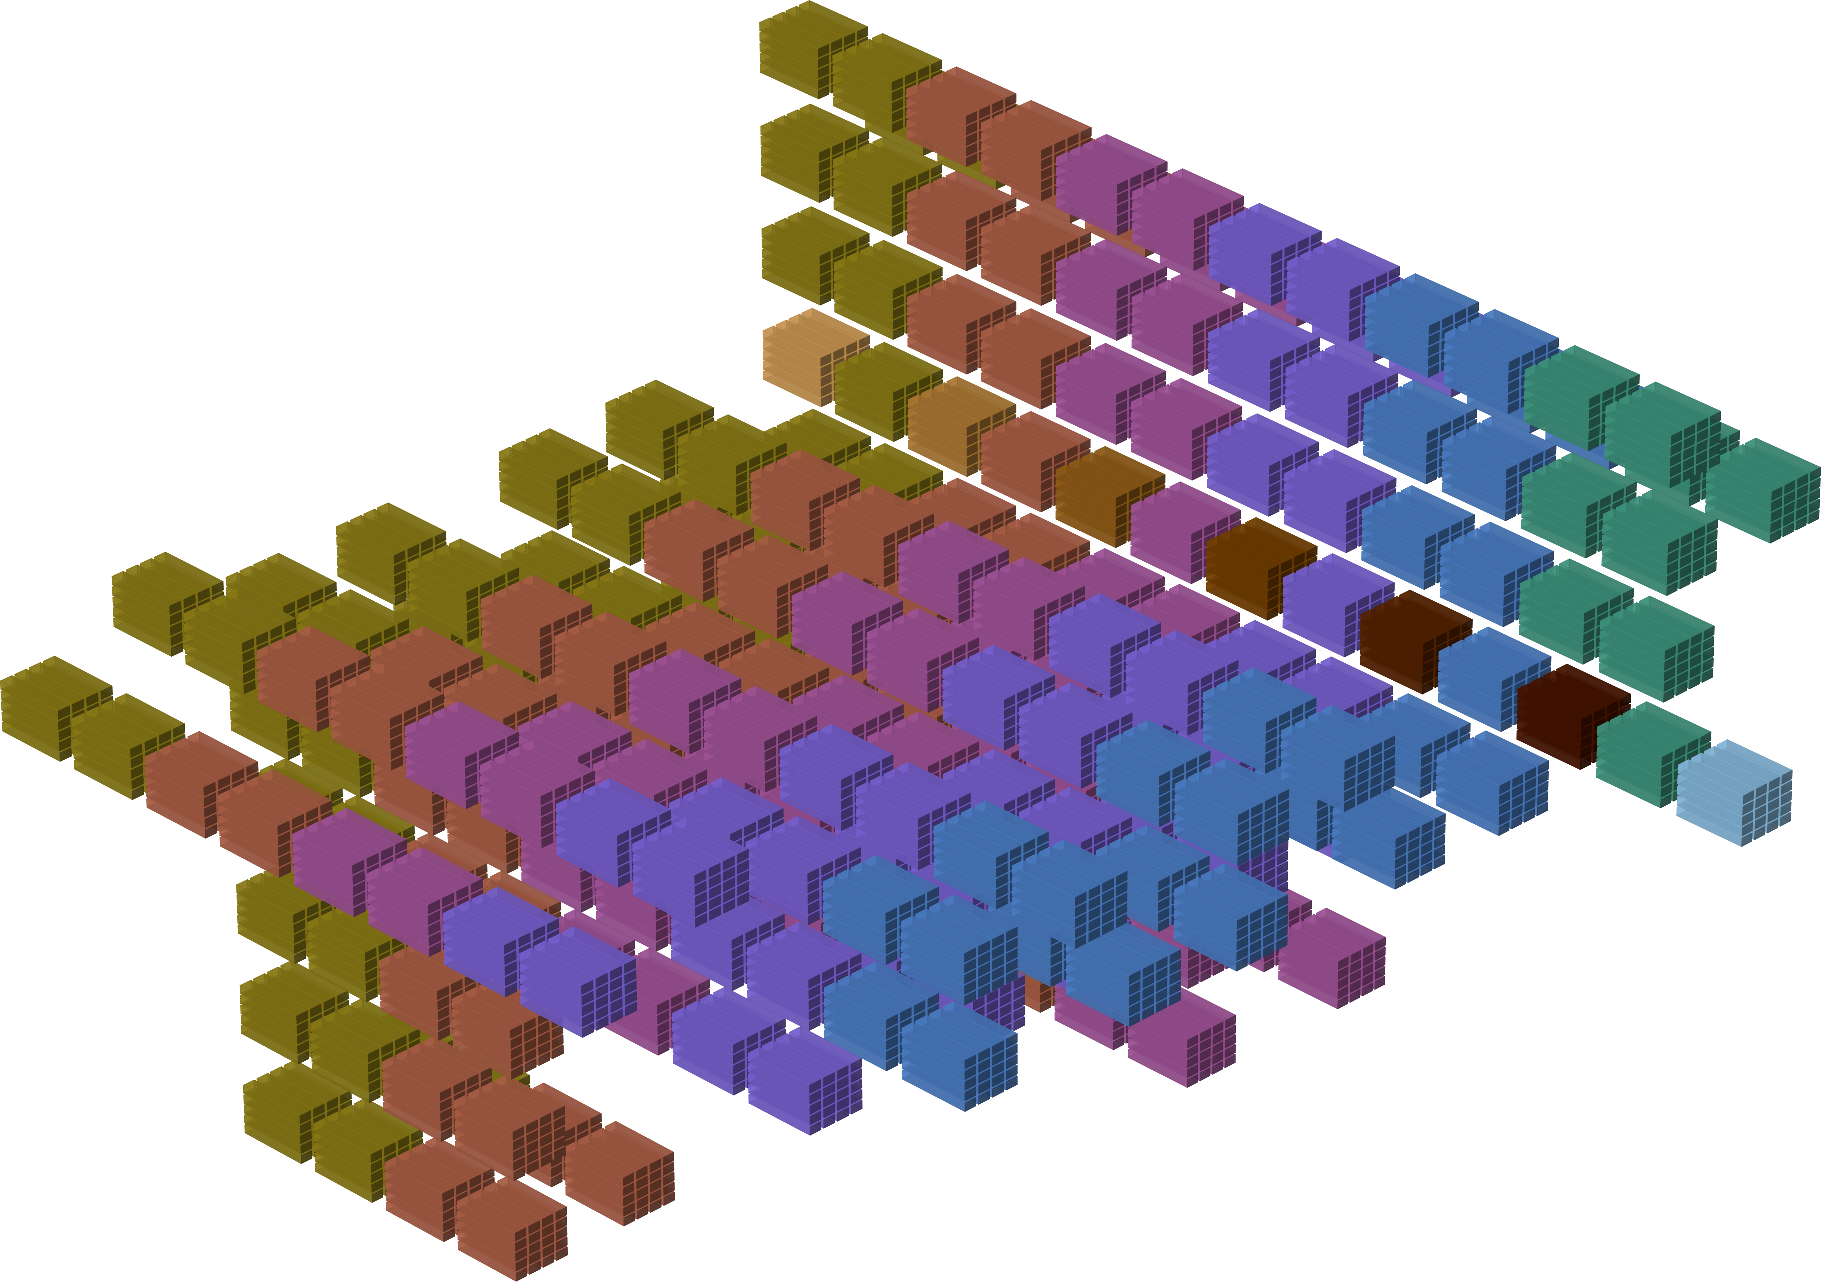
\includegraphics[width=10cm]{src/colorspace_patterns/pattern15-225.png}%
    \end{adjustbox}
\caption{'User LightForm 7'.}
\end{figure}
\end{minipage}
\begin{minipage}[b]{0.68\linewidth}
\begin{lrbox}{\mybox}%
\begin{lstlisting}[basicstyle=\ttfamily\tiny,escapechar=\%]
userLightform7XPosArray
.BYTE $00,$00,$00,$FE,$55                        ;    1              
.BYTE $00,$02,$05,$07,$0A,$03,$05,$08,$0A,$55    ;                   
.BYTE $0C,$0E,$00,$02,$05,$07,$0A,$55            ;  1 6              
.BYTE $00,$00,$00,$FD,$55                        ;                   
.BYTE $0A,$0A,$0A,$08,$55                        ;    1              
.BYTE $00,$55                                    ;                3  
userLightform7YPosArray                          ;       2 2  2 2   3
.BYTE $FE,$FC,$FA,$FC,$55                        ;                   
.BYTE $02,$02,$02,$02,$02,$00,$00,$00,$00,$55    ;    2 2  2 2  2    
.BYTE $FF,$00,$04,$04,$04,$04,$04,$55            ;                   
.BYTE $06,$08,$0A,$0A,$55                        ;    3 3  3 3  3    
.BYTE $06,$08,$0A,$0A,$55                        ;                   
.BYTE $FC,$55                                    ;    4         5    
.BYTE $55                                        ;                   
.BYTE $55                                        ;    4         5    
.BYTE $55                                        ;                   
        .BYTE $55                                        ; 4  4       5 5    
\end{lstlisting}
\end{lrbox}%
\scalebox{0.8}{\usebox{\mybox}}
\subfile{colorspace_patterns/tables/pattern15.tex}
\end{minipage}
%
%
\begin{minipage}[b]{0.48\linewidth}
\vspace{1cm}
\begin{figure}[H]
    \centering
    \begin{adjustbox}{width=5cm,margin=0cm 0cm}
      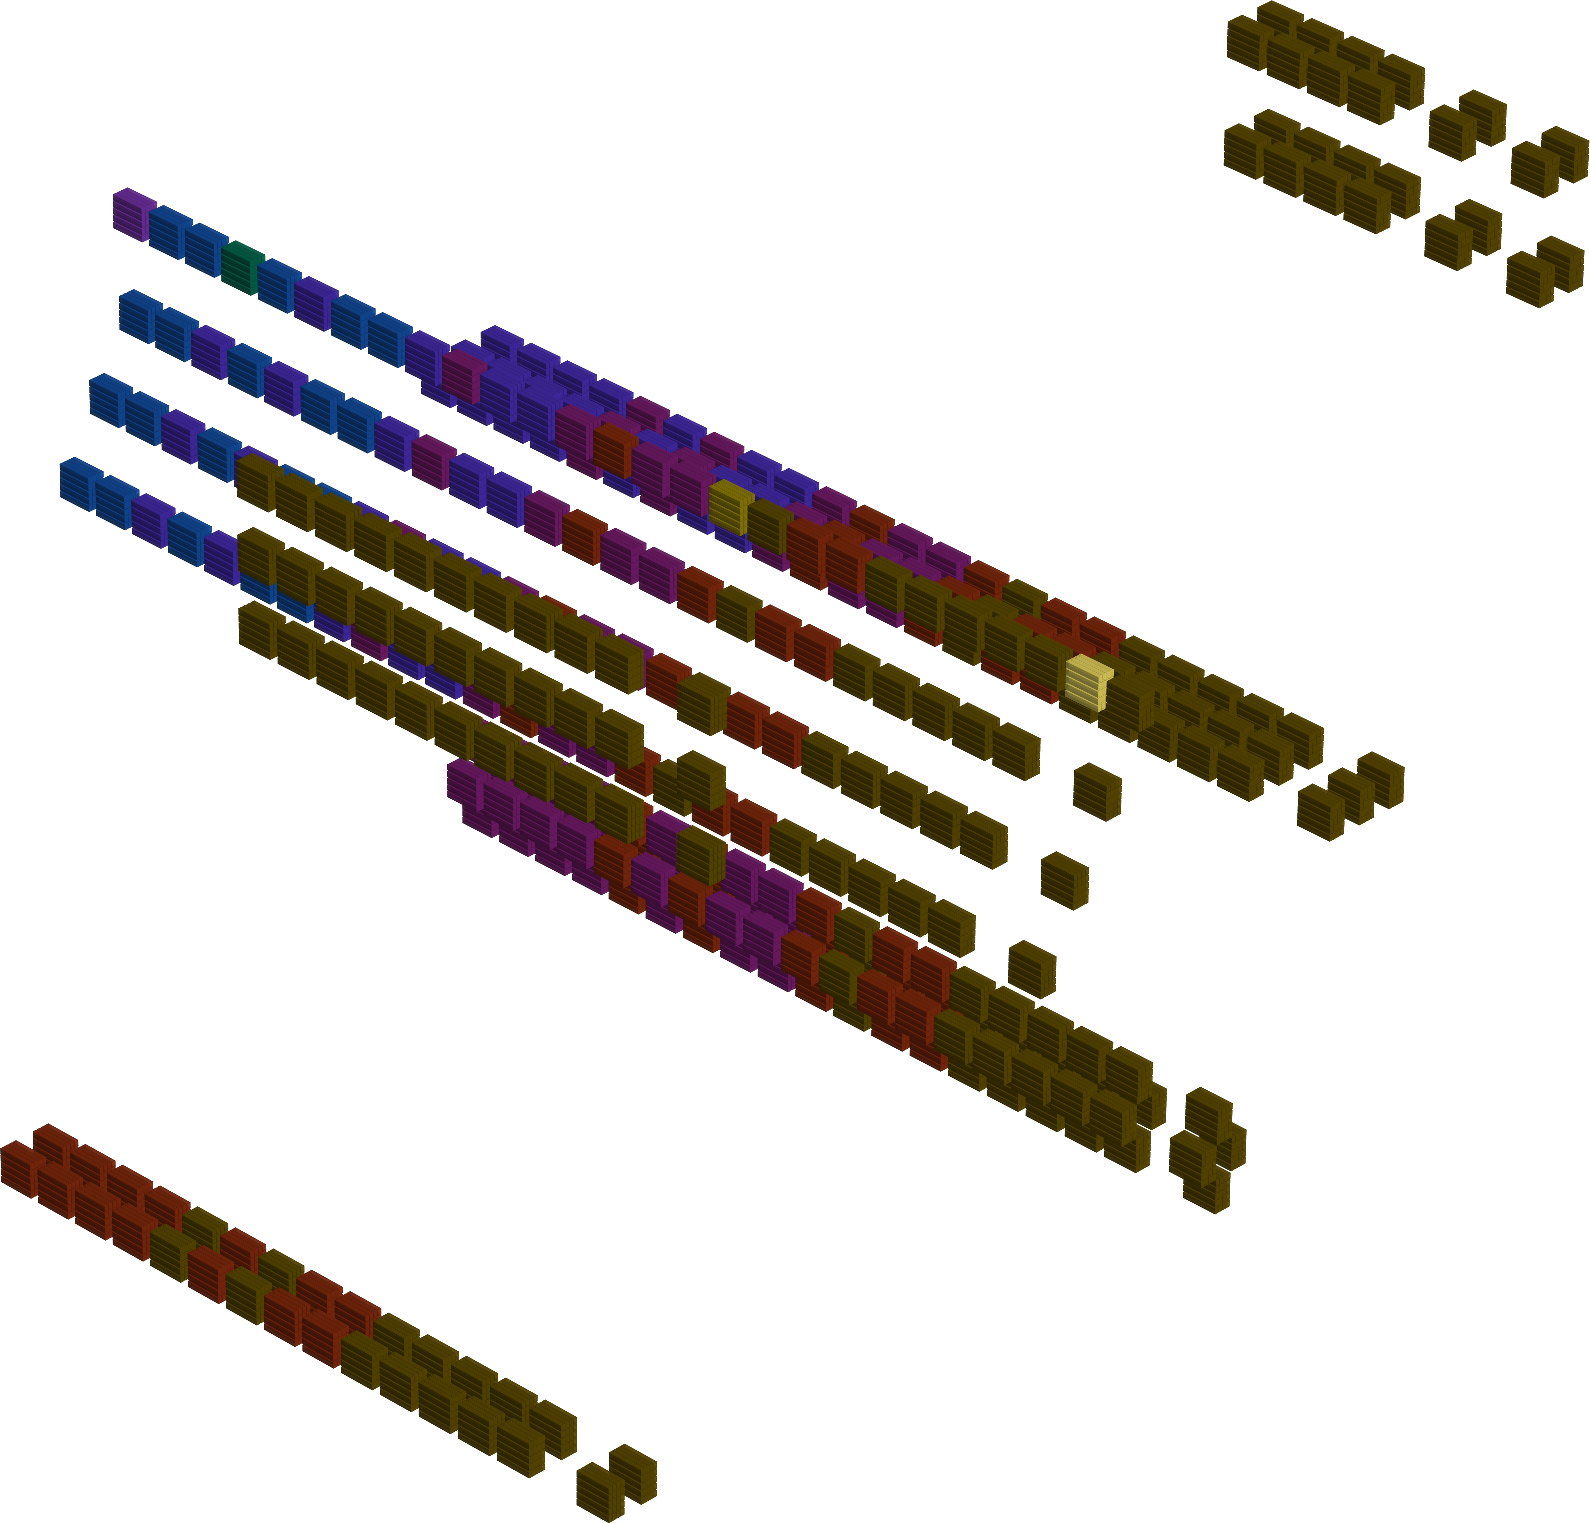
\includegraphics[width=10cm]{src/colorspace_patterns/pattern16-45.png}%
    \end{adjustbox}
    \begin{adjustbox}{width=5cm,margin=0cm 0cm}
      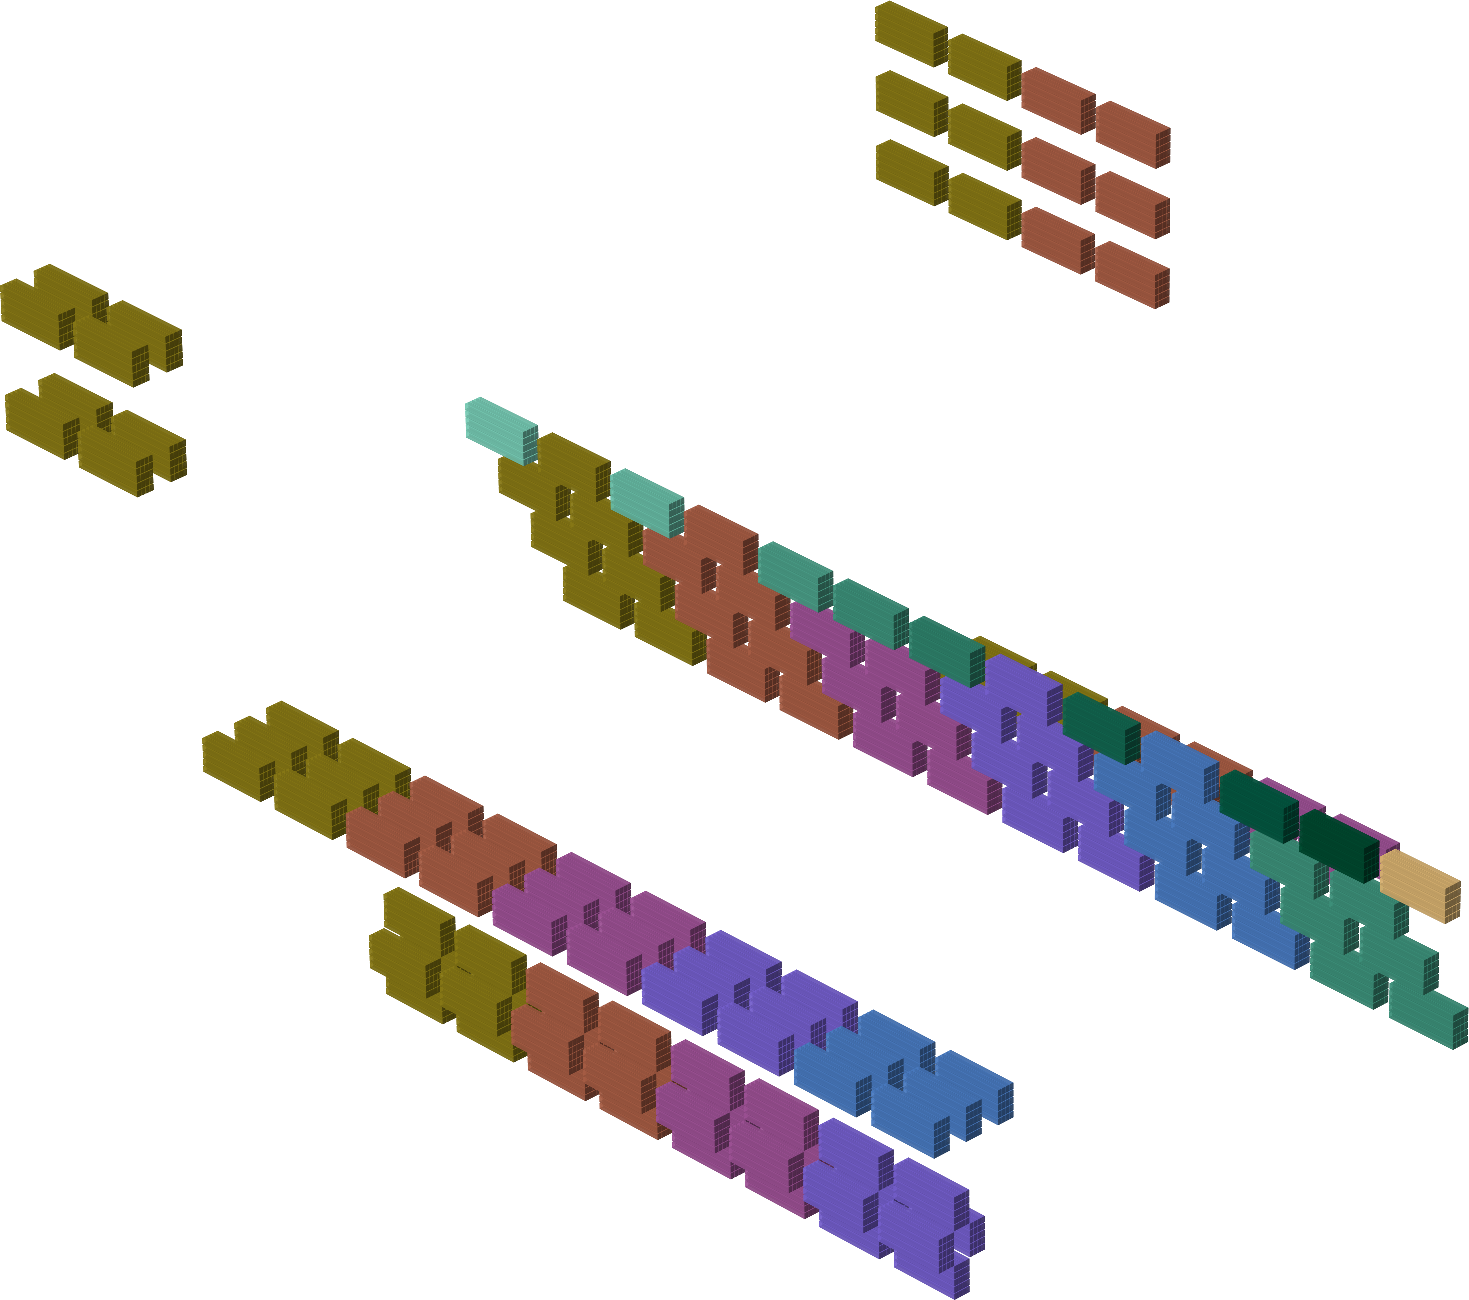
\includegraphics[width=10cm]{src/colorspace_patterns/pattern16-225.png}%
    \end{adjustbox}
\caption{'User LightForm 8'.}
\end{figure}
\end{minipage}
\begin{minipage}[b]{0.68\linewidth}
\vspace{1cm}
\begin{lrbox}{\mybox}%
\begin{lstlisting}[basicstyle=\ttfamily\tiny,escapechar=\%]
userLightform8XPosArray
.BYTE $FE,$FC,$FA,$55      ;                                                            6 6
.BYTE $0D,$0F,$11,$55      ;                                                               
.BYTE $06,$05,$07,$06,$55  ;                                                               
.BYTE $DF,$E1,$55          ;       5                                                    6 6
.BYTE $E5,$E5,$E5,$55      ;                                                               
.BYTE $1A,$1C,$1C,$1A,$55  ;       5                                                       
userLightform8YPosArray            ;                                                                   
.BYTE $02,$04,$06,$55      ;       5                                                       
.BYTE $06,$06,$06,$55      ;                                                               
.BYTE $0D,$0E,$0E,$0F,$55  ;                                                               
.BYTE $0E,$0E,$55          ;                                                               
.BYTE $FA,$FC,$FE,$55      ;                                1                              
.BYTE $F7,$FA,$F7,$FA,$55  ;                                                               
.BYTE $55                  ;                              1                                
.BYTE $55                  ;                                                               
.BYTE $55                  ;                            1                  2 2 2           
.BYTE $55                  ;                                                               
.BYTE $55                  ;                                                               
.BYTE $55                  ;                                                               
.BYTE $55                  ;                                                               
.BYTE $55                  ;                                                               
.BYTE $55                  ;                                                               
.BYTE $55                  ;                                        3                      
.BYTE $55                  ; 4 4                                   3 3                     
.BYTE $55                  ;                                        3                      
\end{lstlisting}
\end{lrbox}%
\scalebox{0.8}{\usebox{\mybox}}
\subfile{colorspace_patterns/tables/pattern16.tex}
\end{minipage}
%
\clearpage
\textbf{Lines 1189-1231. \icode{\textbf{PaintPixel}}} 
\begin{lstlisting}[basicstyle=\ttfamily\scriptsize, caption=The routine responsible for painting patterns.]
PaintPixel
        LDX previousPixelYPosition
        PHA 
        LDY previousPixelXPosition
        TXA 
        AND #$80
        BNE ReturnEarlyFromPaintPixel
        CPX #NUM_COLS + $0A
        BPL ReturnEarlyFromPaintPixel
        TYA 
        AND #$80
        BNE ReturnEarlyFromPaintPixel

        CPY #NUM_COLS
        BPL ReturnEarlyFromPaintPixel

        LDA backgroundLinePtrLoArray,X
        STA linePtrLo
        LDA backgroundLinePtrHiArray,X
        STA linePtrHi
        LDA foregroundPixelsLoPtrArray,X
        STA foregroundLoPtr
        LDA foregroundPixelsHiPtrArray,X
        STA foregroundHiPtr

        PLA 
        STA pixelValueToPaint

        LDA beginDrawingForeground
        BNE ActuallyPaintPixel

        LDA (linePtrLo),Y
        AND #$EF
        SEC 
        SBC pixelValueToPaint
        BMI ActuallyPaintPixel

        CMP #$01
        BEQ ActuallyPaintPixel
        RTS 

        ; Each pixel is a four bit nibble. The nibble is then an index
        ; into presetColorValuesArray giving the color for the 'pixel'.
ActuallyPaintPixel   
        LDA pixelValueToPaint
        STA (linePtrLo),Y
        AND #$0F
        PHA 
        TYA 
        CLC 
        ROR 
        BCC PaintForegroundPixels
        TAY 
        PLA 
        STA pixelValueToPaint
        LDA (foregroundLoPtr),Y
        AND #$F0
        ORA pixelValueToPaint
        STA (foregroundLoPtr),Y
        RTS 
\end{lstlisting}
\clearpage

\rhead[]{\icode{PaintPixel}}
\textbf{Lines 1189-1231. \icode{\textbf{PaintPixel}}:} We've already encountered this routine
in \hyperref[sec:listing_commentary]{\textcolor{blue}{ our walk through of the listing.}}. This is the version that shipped 
with the commercial edition of Psychedelia so has a necessary extra complication to deal with the fact that we 
are going to paint one of up to 16 possible patterns. What we want to figure out here is the X and Y position we should
paint for each element in the pattern's data structure.
\clearpage

%
\begin{minipage}[b]{0.48\linewidth}
\begin{figure}[H]
    \centering
    \begin{adjustbox}{width=4cm,margin=0cm 0cm}
      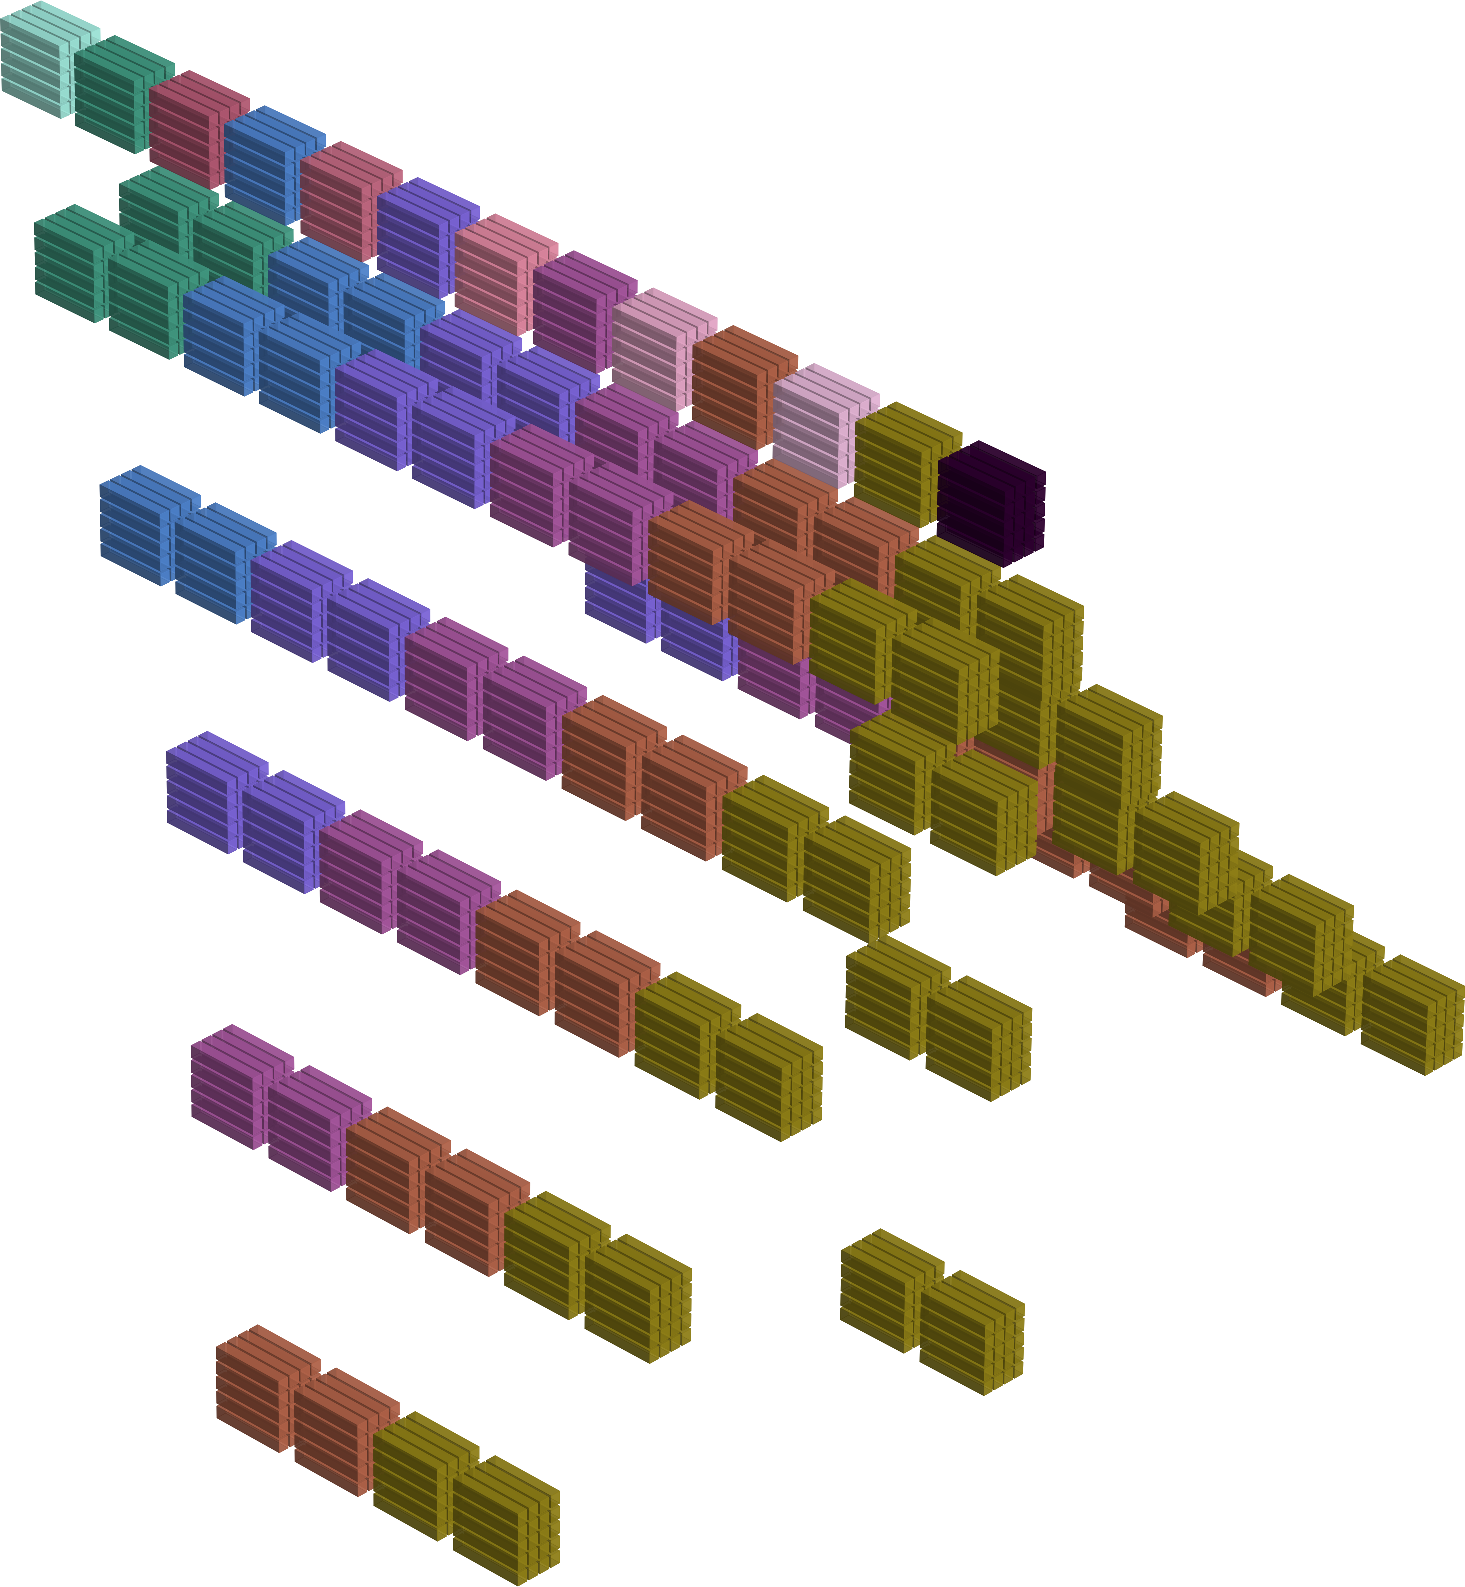
\includegraphics[width=10cm]{src/colorspace_patterns/pattern17-45.png}%
    \end{adjustbox}
    \begin{adjustbox}{width=4cm,margin=0cm 0cm}
      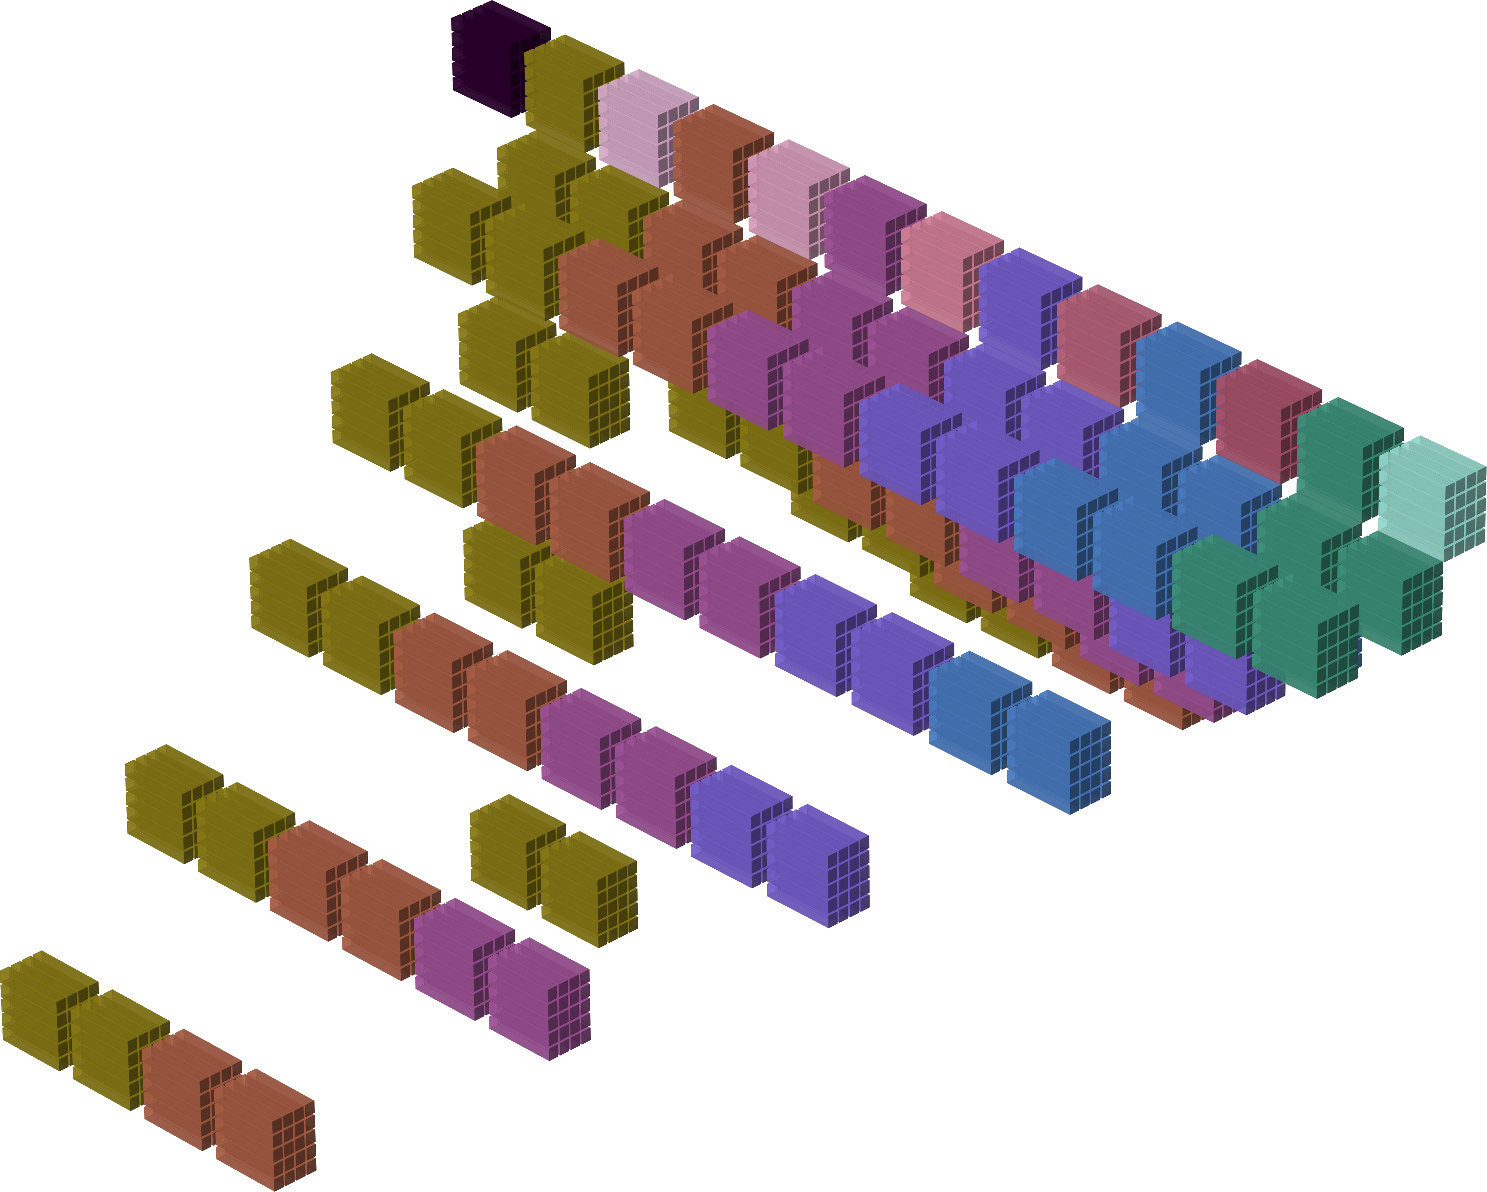
\includegraphics[width=10cm]{src/colorspace_patterns/pattern17-225.png}%
    \end{adjustbox}
\caption{'User LightForm 9'.}
\end{figure}
\end{minipage}
\begin{minipage}[b]{0.48\linewidth}
\begin{lrbox}{\mybox}%
\hspace{1cm}
\begin{lstlisting}[basicstyle=\ttfamily\tiny,escapechar=\%]
userLightform9XPosArray
.BYTE $FF,$01,$55         ;                        
.BYTE $FD,$03,$55         ;                        
.BYTE $FB,$05,$55         ;           1 1          
.BYTE $F8,$08,$55         ;                        
.BYTE $F5,$0B,$55         ;         2  6  2        
.BYTE $00,$00,$00,$55     ;                        
userLightform9YPosArray           ;       3         3      
.BYTE $02,$02,$55         ;            6           
.BYTE $04,$04,$55         ;    4               4   
.BYTE $06,$06,$55         ;                        
.BYTE $08,$08,$55         ; 5                     5
.BYTE $0A,$0A,$55         ;            6           
.BYTE $04,$07,$0B,$55
\end{lstlisting}
\end{lrbox}%
\scalebox{0.8}{\usebox{\mybox}}
\subfile{colorspace_patterns/tables/pattern17.tex}
\end{minipage}
%
%
\begin{minipage}[b]{0.48\linewidth}
\vspace{2cm}
\begin{figure}[H]
    \centering
    \begin{adjustbox}{width=4cm,margin=0cm 0cm}
      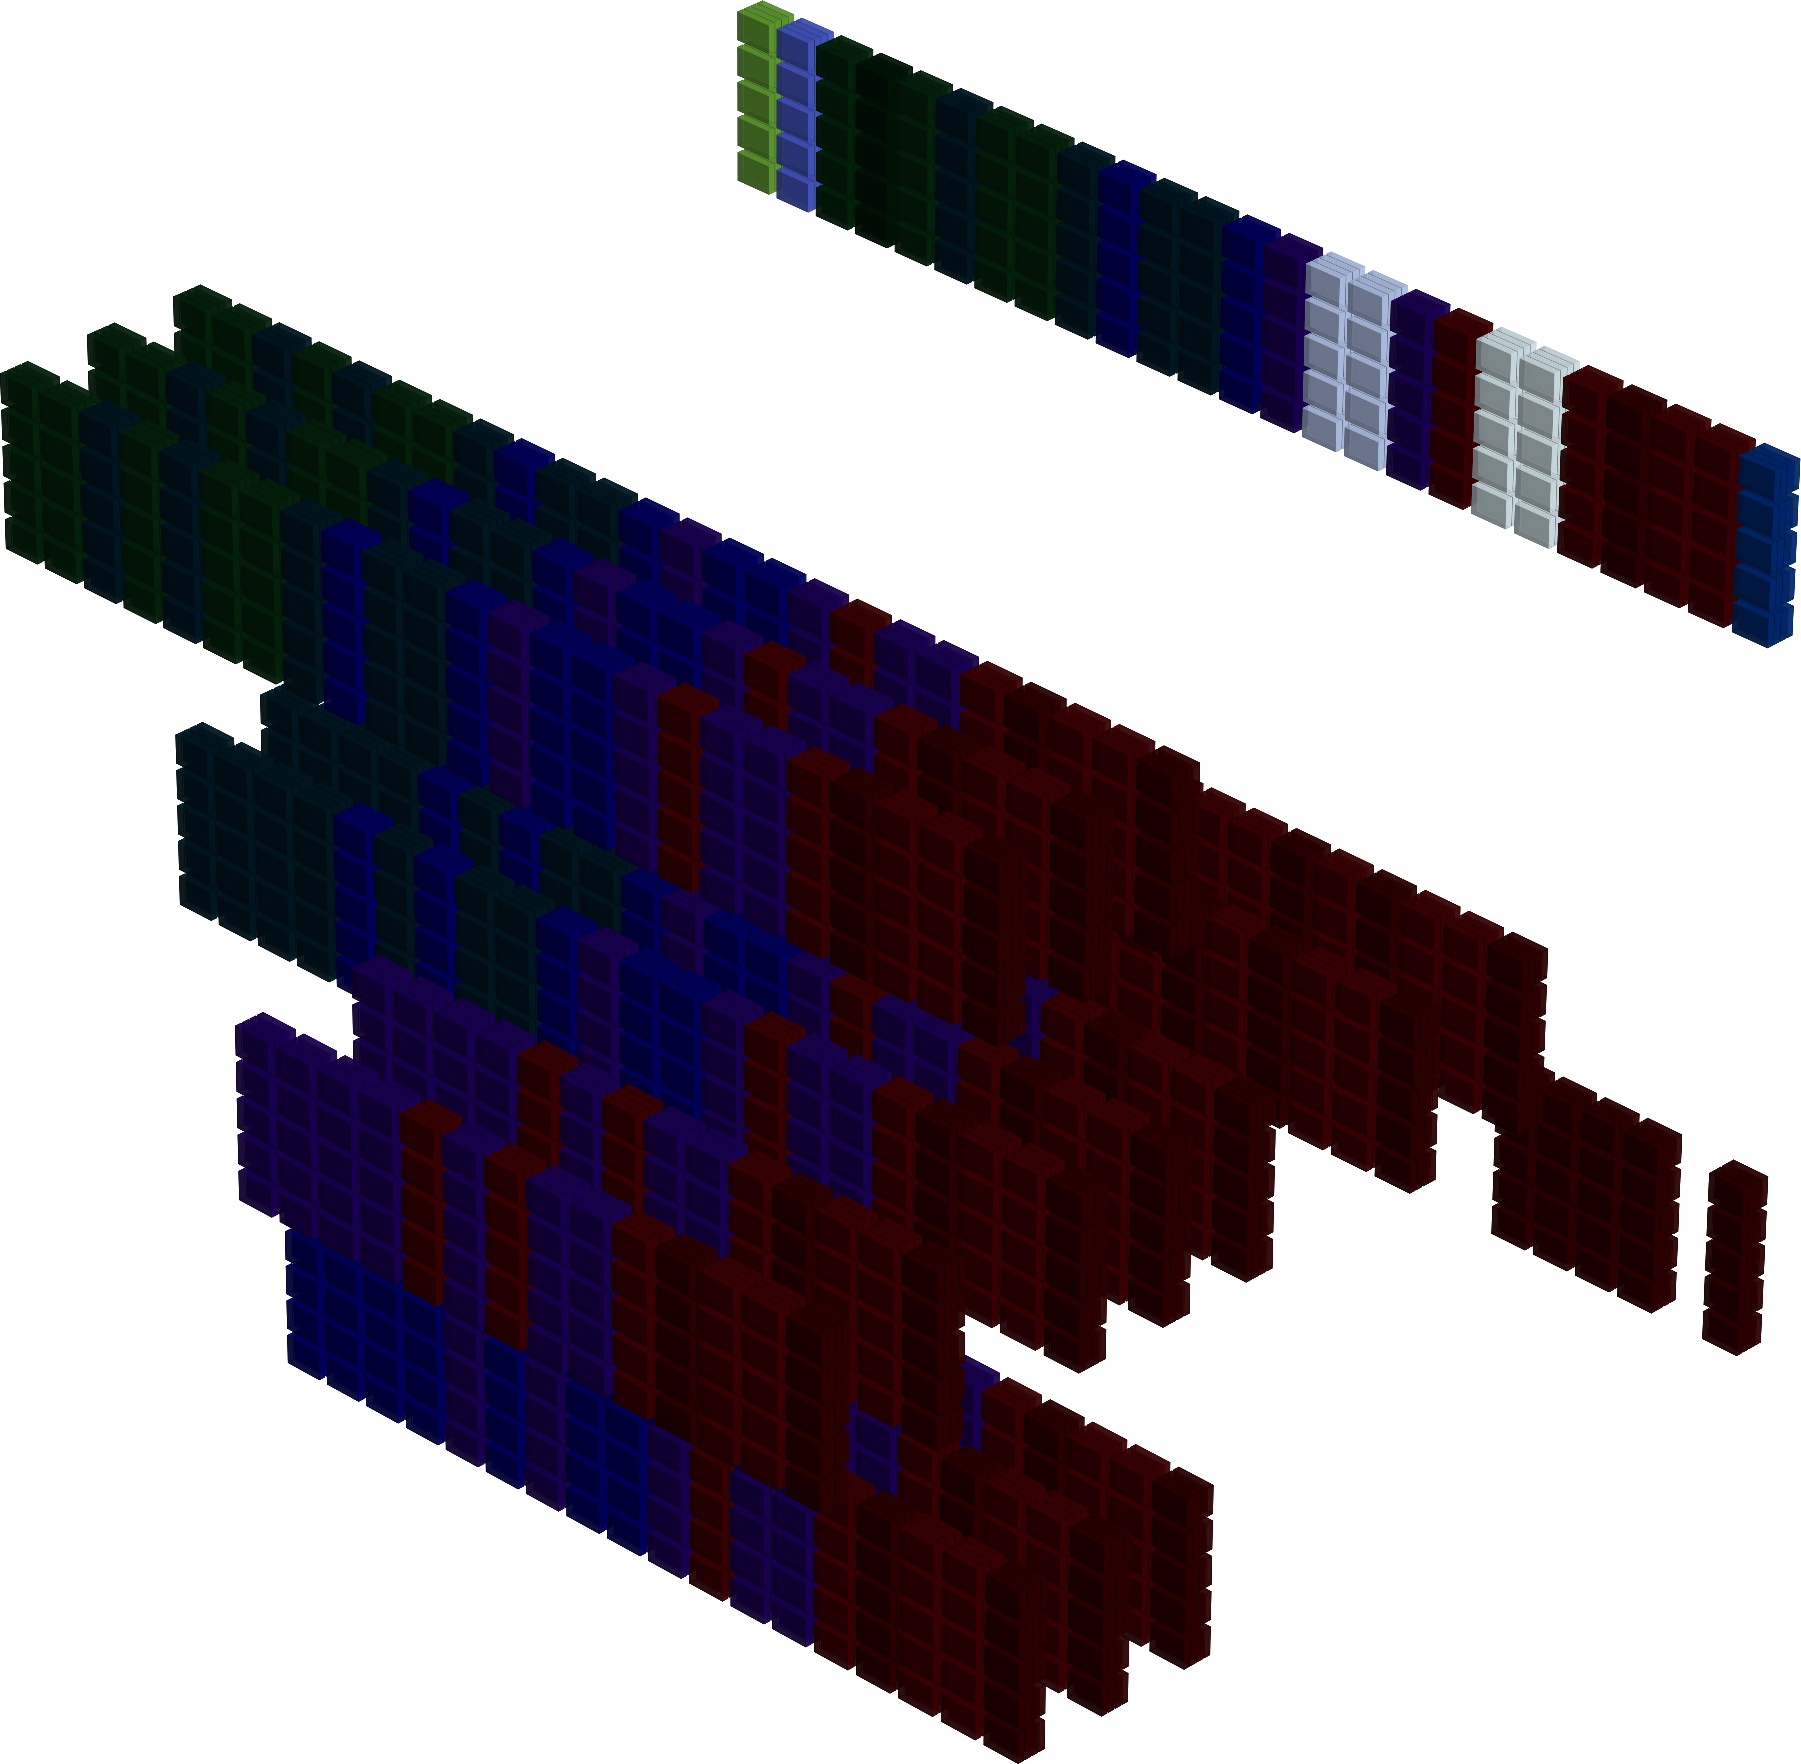
\includegraphics[width=10cm]{src/colorspace_patterns/pattern18-45.png}%
    \end{adjustbox}
    \begin{adjustbox}{width=4cm,margin=0cm 0cm}
      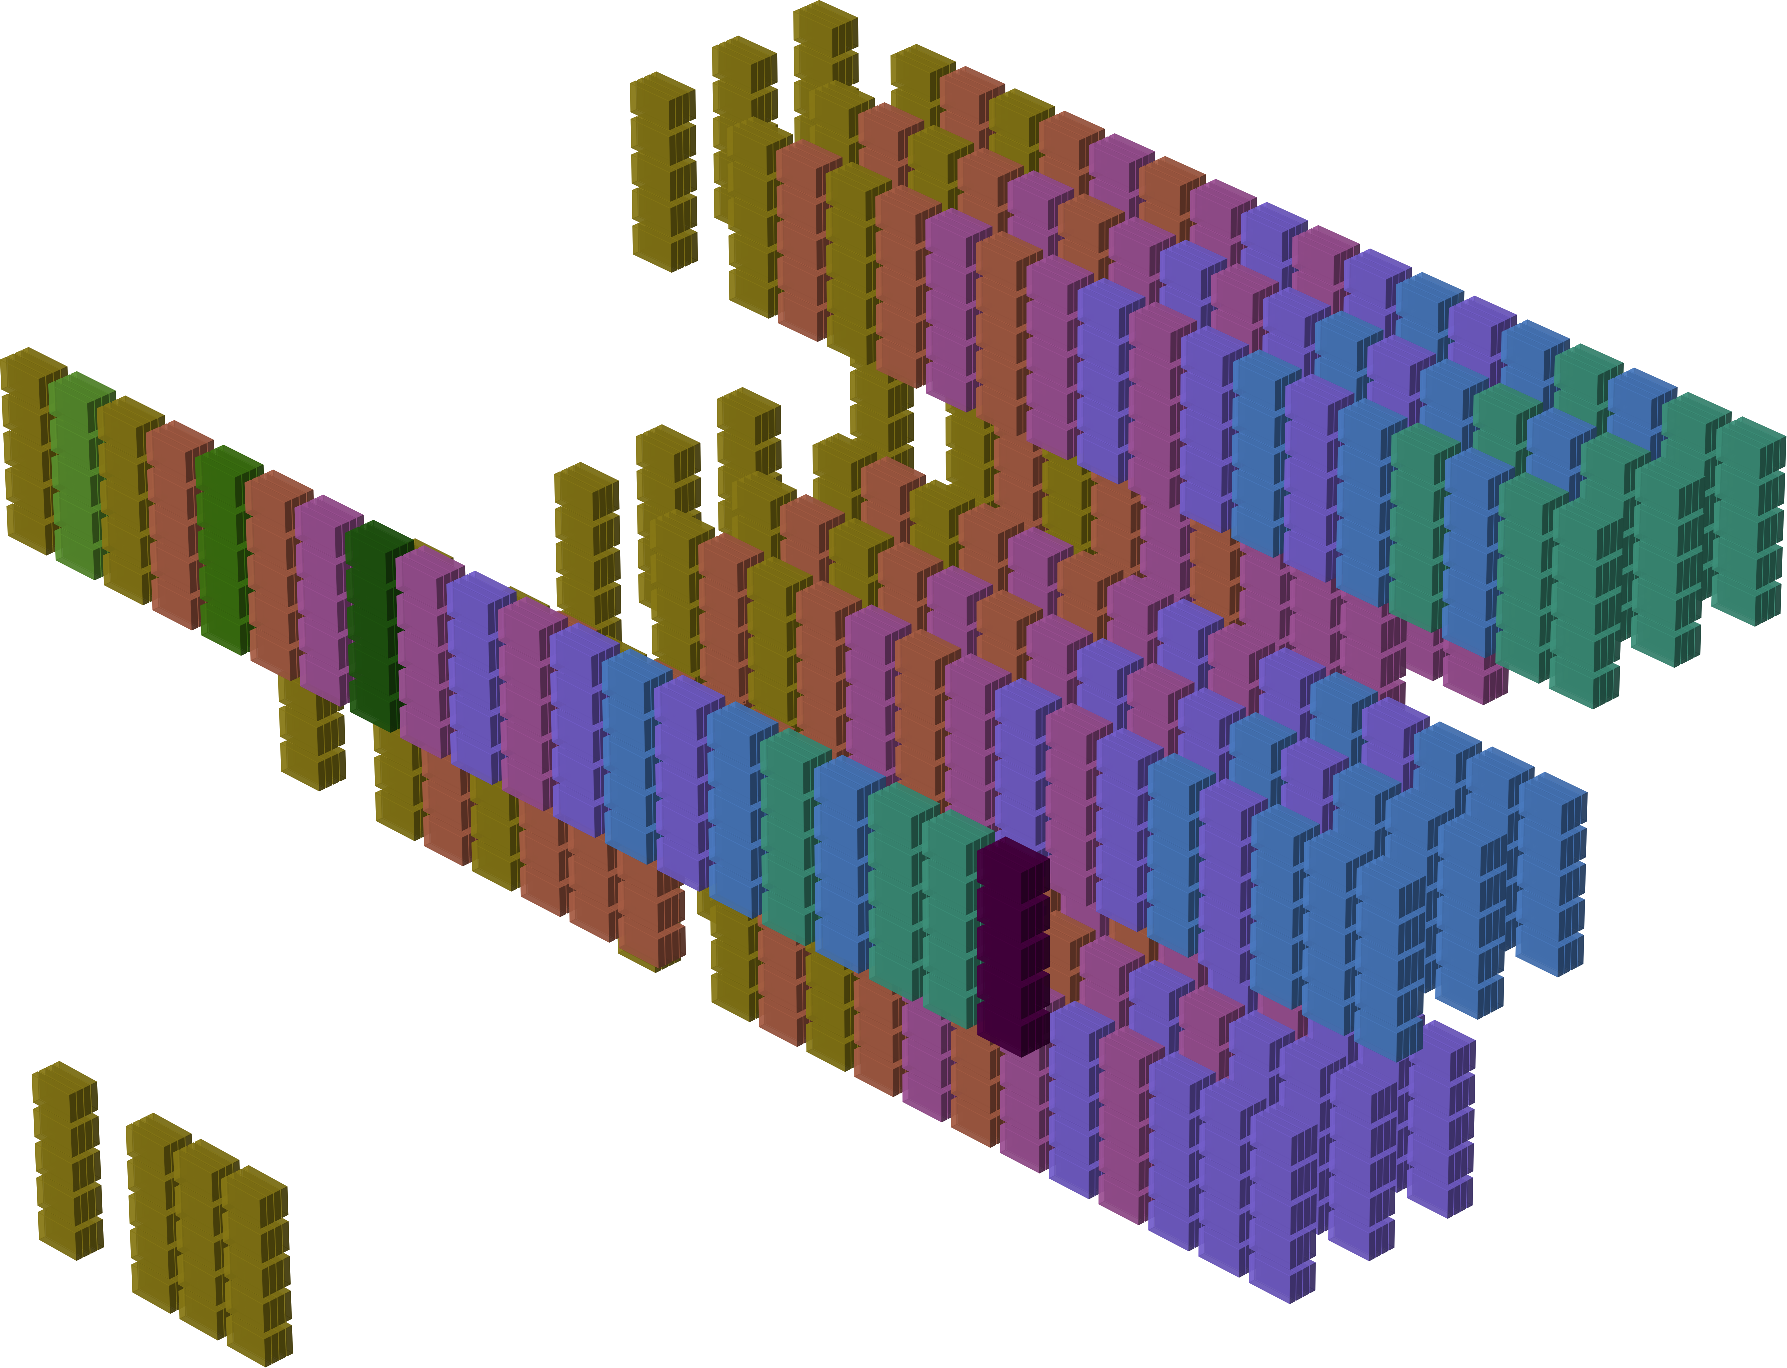
\includegraphics[width=10cm]{src/colorspace_patterns/pattern18-225.png}%
    \end{adjustbox}
\caption{'User LightForm 10'.}
\end{figure}
\end{minipage}
\begin{minipage}[b]{0.58\linewidth}
\vspace{2cm}
\begin{lrbox}{\mybox}%
\hspace{1cm}
\begin{lstlisting}[basicstyle=\ttfamily\tiny,escapechar=\%]
userLightform10XPosArray
.BYTE $EA,$E7,$E4,$55    ;       1  1  1                      
.BYTE $E7,$EA,$ED,$55    ;                                    
.BYTE $E5,$E8,$EB,$55    ; 4   4    2  2  2     5   5         
.BYTE $E2,$DE,$55        ;                                    
.BYTE $F3,$F7,$55        ;        3  3  3                    6
.BYTE $00,$55
userLightform10YPosArray
.BYTE $00,$00,$00,$55
.BYTE $02,$02,$02,$55
.BYTE $04,$04,$04,$55
.BYTE $02,$02,$55
.BYTE $02,$02,$55
.BYTE $04,$55
\end{lstlisting}
\end{lrbox}%
\scalebox{0.8}{\usebox{\mybox}}
\subfile{colorspace_patterns/tables/pattern18.tex}
\end{minipage}
%
%
\begin{minipage}[b]{0.48\linewidth}
\begin{figure}[H]
    \centering
    \begin{adjustbox}{width=5cm,margin=0cm 0cm}
      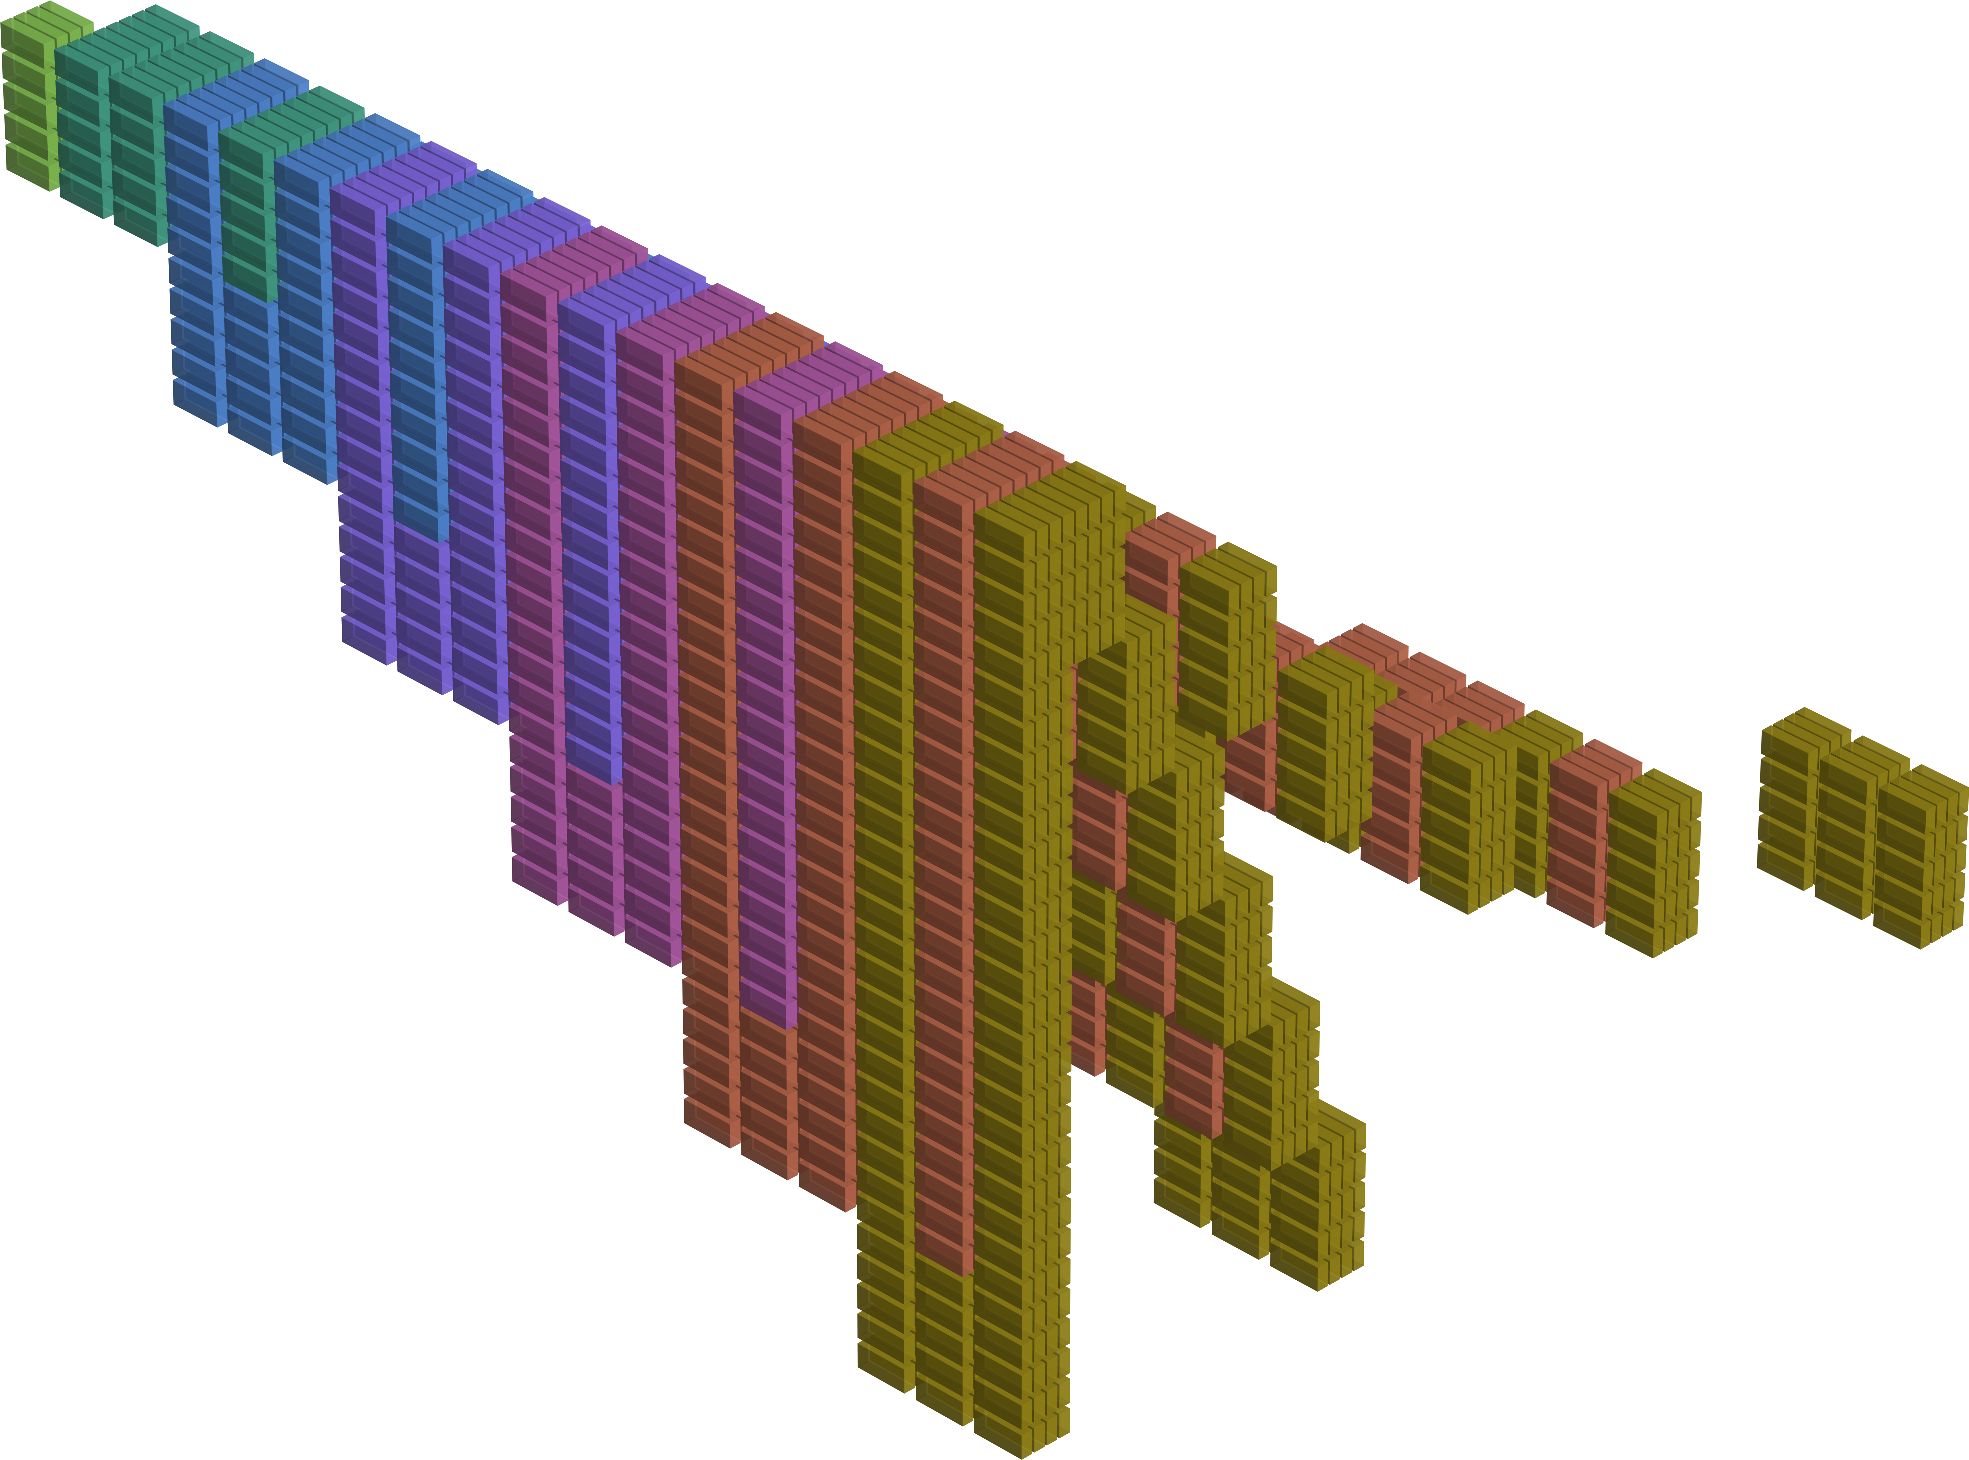
\includegraphics[width=10cm]{src/colorspace_patterns/pattern19-45.png}%
    \end{adjustbox}
    \begin{adjustbox}{width=5cm,margin=0cm 0cm}
      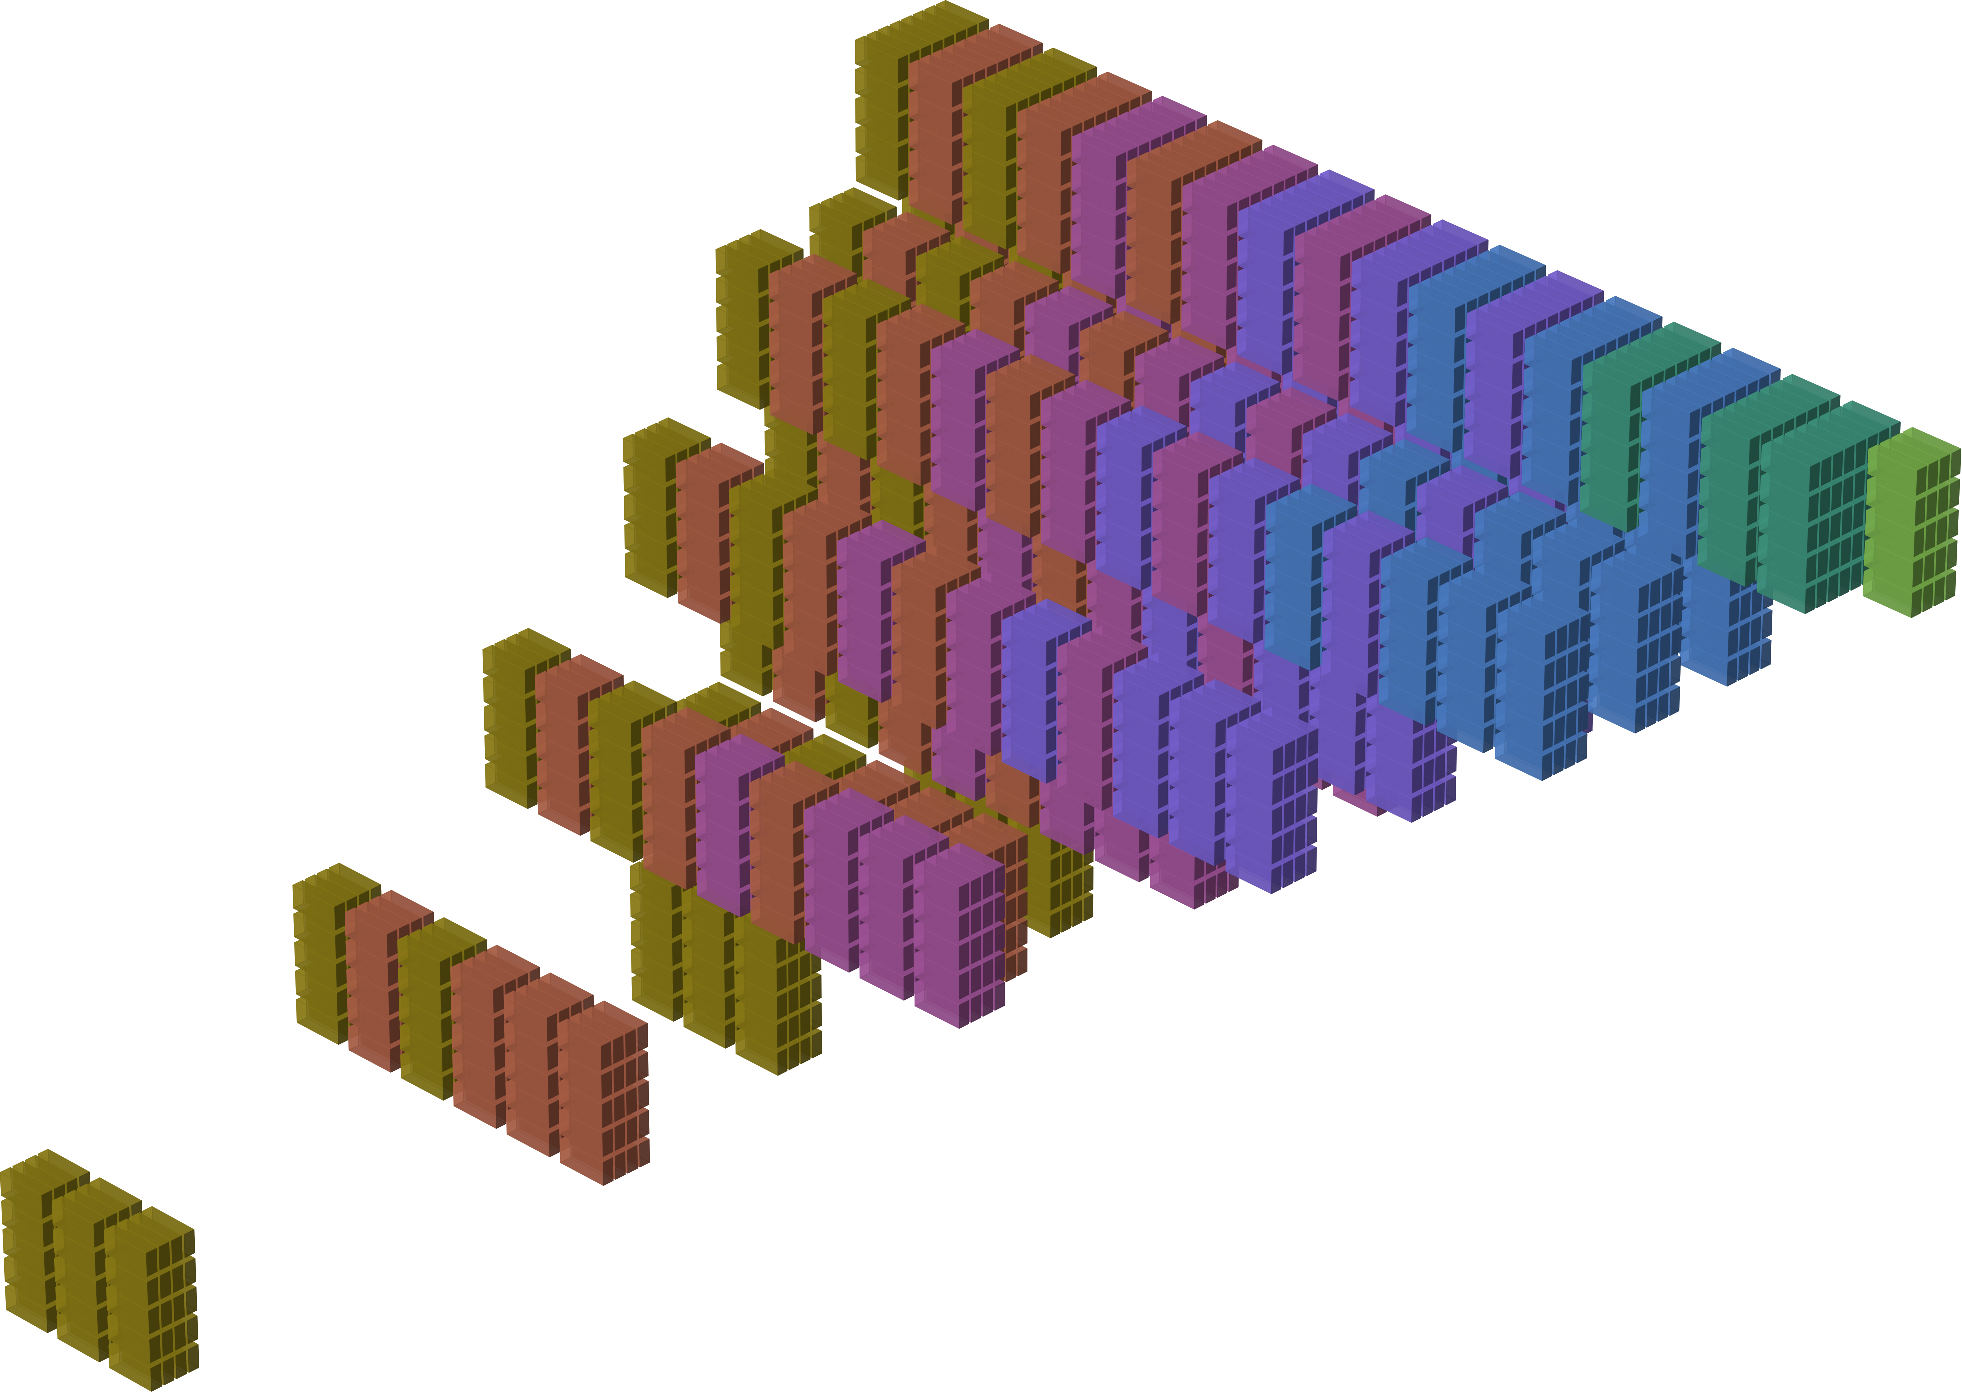
\includegraphics[width=10cm]{src/colorspace_patterns/pattern19-225.png}%
    \end{adjustbox}
\caption{'User LightForm 11'.}
\end{figure}
\end{minipage}
\begin{minipage}[b]{0.48\linewidth}
\begin{lrbox}{\mybox}%
\hspace{1cm}
\begin{lstlisting}[basicstyle=\ttfamily\tiny,escapechar=\%]
userLightform11XPosArray
        .BYTE $01,$55           ;  1                  
        .BYTE $00,$02,$04,$55   ; 2 2 2               
        .BYTE $00,$03,$06,$55   ; 3  3  3             
        .BYTE $00,$04,$09,$55   ; 4   4    4          
        .BYTE $00,$05,$0D,$55   ; 5    5       5      
        .BYTE $00,$06,$13,$55   ; 6     6            6
userLightform11YPosArray
        .BYTE $00,$55
        .BYTE $01,$01,$01,$55
        .BYTE $02,$02,$02,$55
        .BYTE $03,$03,$03,$55
        .BYTE $04,$04,$04,$55
        .BYTE $05,$05,$05,$55
\end{lstlisting}
\end{lrbox}%
\scalebox{0.8}{\usebox{\mybox}}
\subfile{colorspace_patterns/tables/pattern19.tex}
\end{minipage}
%
%
\begin{minipage}[b]{0.48\linewidth}
\vspace{2cm}
\begin{figure}[H]
    \centering
    \begin{adjustbox}{width=4cm,margin=0cm 0cm}
      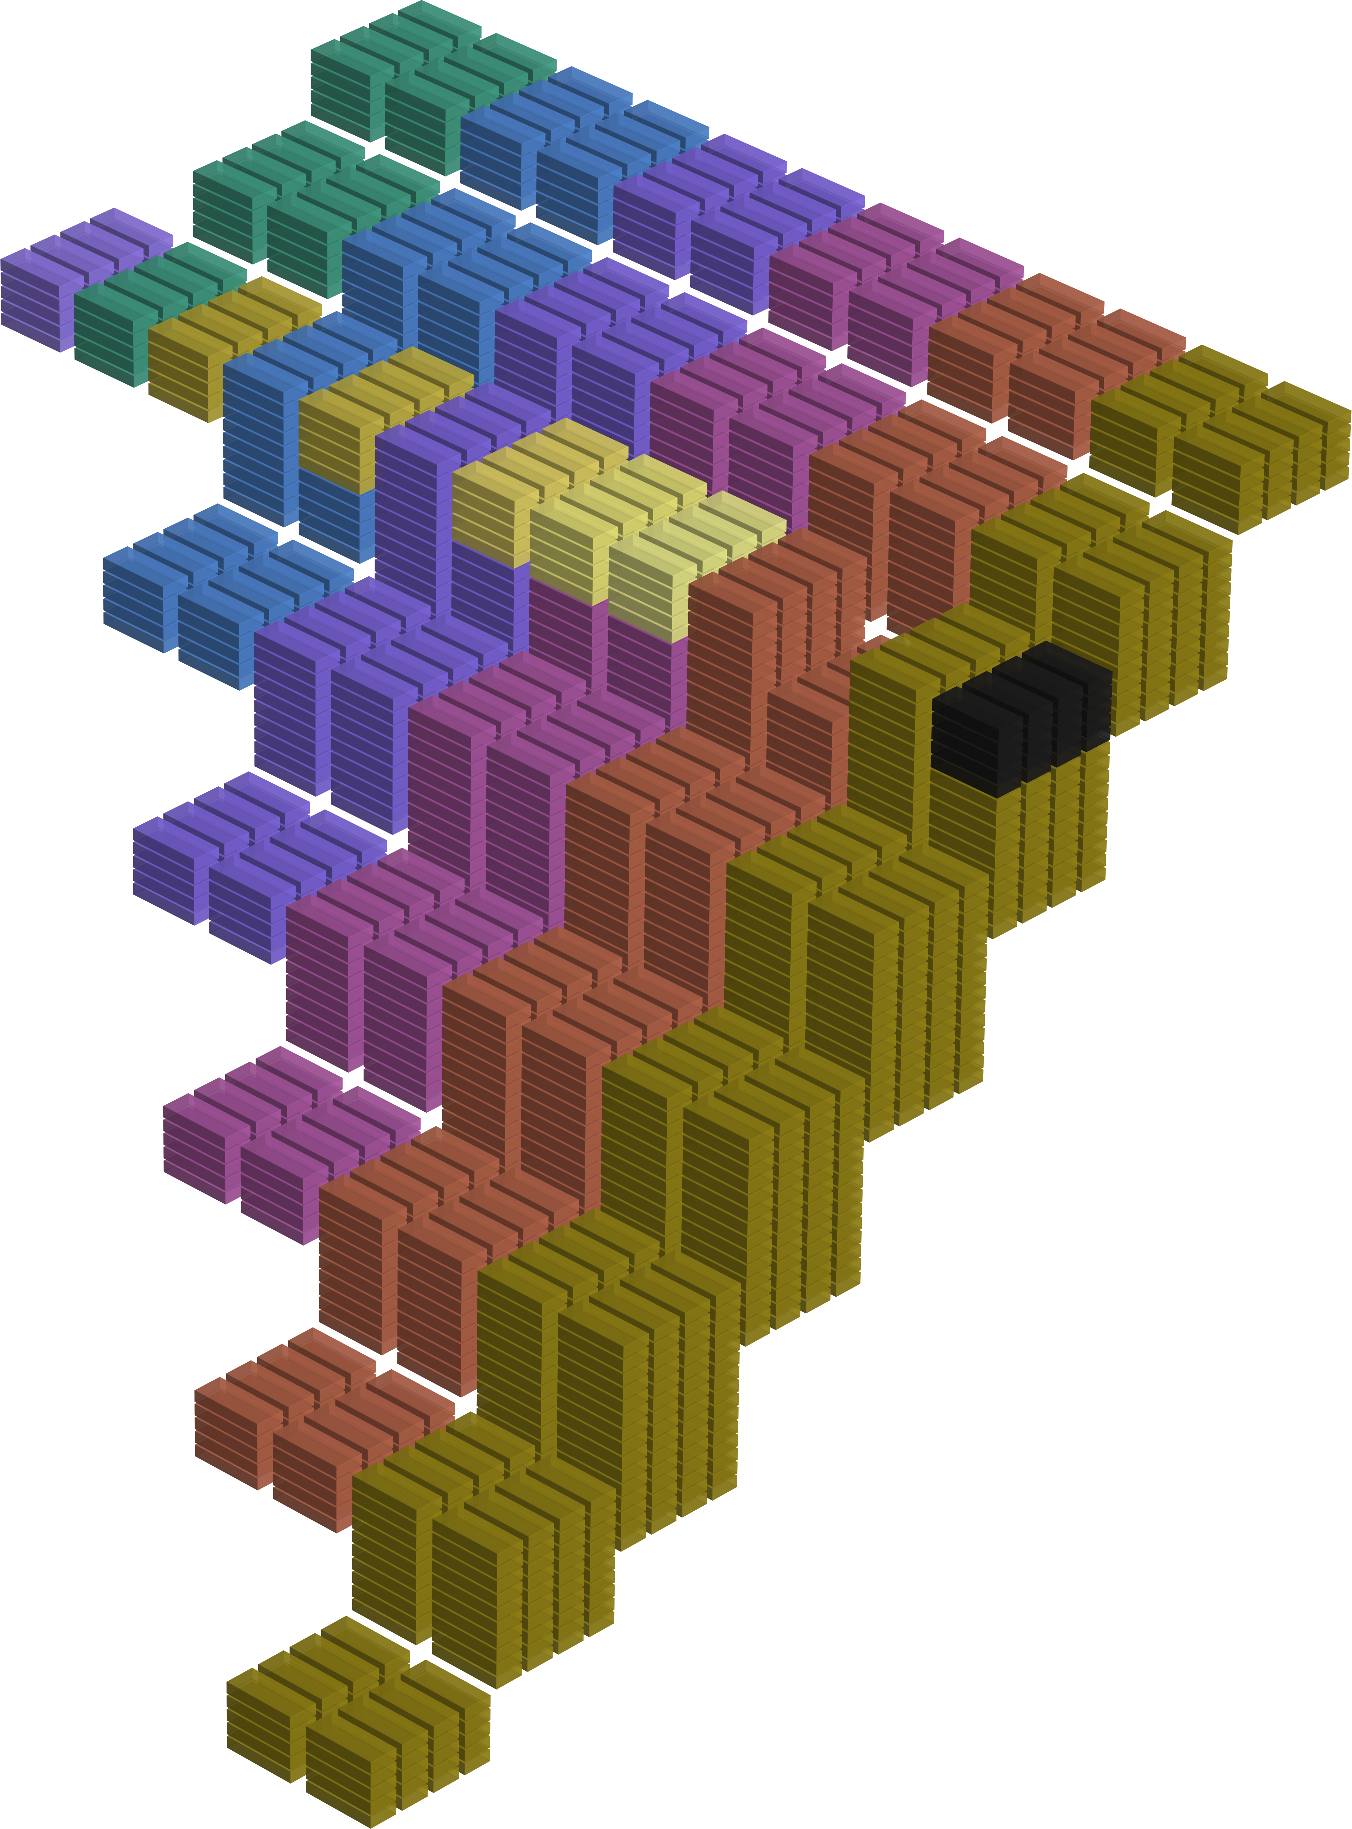
\includegraphics[width=10cm]{src/colorspace_patterns/pattern20-45.png}%
    \end{adjustbox}
    \begin{adjustbox}{width=4cm,margin=0cm 0cm}
      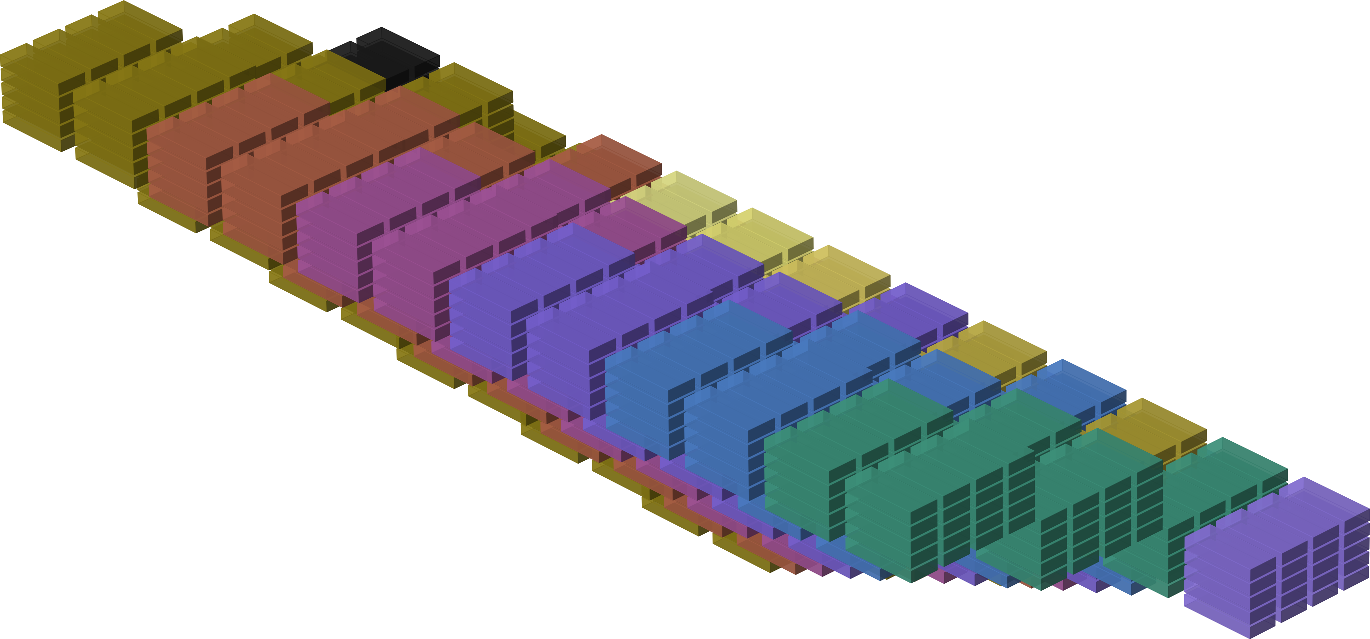
\includegraphics[width=10cm]{src/colorspace_patterns/pattern20-225.png}%
    \end{adjustbox}
\caption{'User LightForm 12'.}
\end{figure}
\end{minipage}
\begin{minipage}[b]{0.48\linewidth}
\vspace{2cm}
\begin{lrbox}{\mybox}%
\hspace{1cm}
\begin{lstlisting}[basicstyle=\ttfamily\tiny,escapechar=\%]
userLightform12XPosArray
.BYTE $01,$02,$55      ;        1
.BYTE $01,$00,$FF,$55  ;       1 
.BYTE $00,$FF,$FE,$55  ;       2 
.BYTE $FF,$FE,$FD,$55  ;      2  
.BYTE $FE,$FD,$FC,$55  ;     23  
.BYTE $FD,$FC,$FB,$55  ;     3   
userLightform12YPosArray;   34  
.BYTE $FF,$FE,$55      ;    4   
.BYTE $00,$01,$02,$55  ;   45   
.BYTE $02,$03,$04,$55  ;   5    
.BYTE $04,$05,$06,$55  ;  56    
.BYTE $06,$07,$08,$55  ;  6     
.BYTE $08,$09,$0A,$55  ; 6      
\end{lstlisting}
\end{lrbox}%
\scalebox{0.8}{\usebox{\mybox}}
\subfile{colorspace_patterns/tables/pattern20.tex}
\end{minipage}
%
\clearpage
\textbf{Lines 1189-1231. \icode{\textbf{CheckKeyboardInput}}} 
\begin{lstlisting}[basicstyle=\ttfamily\scriptsize]
;-------------------------------------------------------
; CheckKeyboardInput
;-------------------------------------------------------
CheckKeyboardInput   
        ...
MaybeSpaceKeyPressed   
        CMP #KEY_SPACE
        BNE MaybeShiftOrControlPressed

        ; Update selected pattern.
        INC currentPatternIndex
        LDA currentPatternIndex
        CMP #$18
        BNE b4E15
        LDA #$00
        STA currentPatternIndex
b4E15   AND #$18
        BEQ b4E26
        LDA currentPatternIndex
        SEC 
        SBC #$08
        STA lastKeyPressed
        LDX #USER_LIGHTFORM_000
        JMP UpdateStatusLineAndDisplaySelectedValue

b4E26   LDX currentPatternIndex
        JMP UpdateStatusLine
\end{lstlisting}
\clearpage

\rhead[]{\icode{CheckKeyboardInput}}
\textbf{Lines 1189-1231. \icode{\textbf{SpacePressed}}:} This is the routine that detects when the player has selected a new
\clearpage
%
%
\begin{minipage}[b]{0.48\linewidth}
\begin{figure}[H]
    \centering
    \begin{adjustbox}{width=5cm,margin=0cm 0cm}
      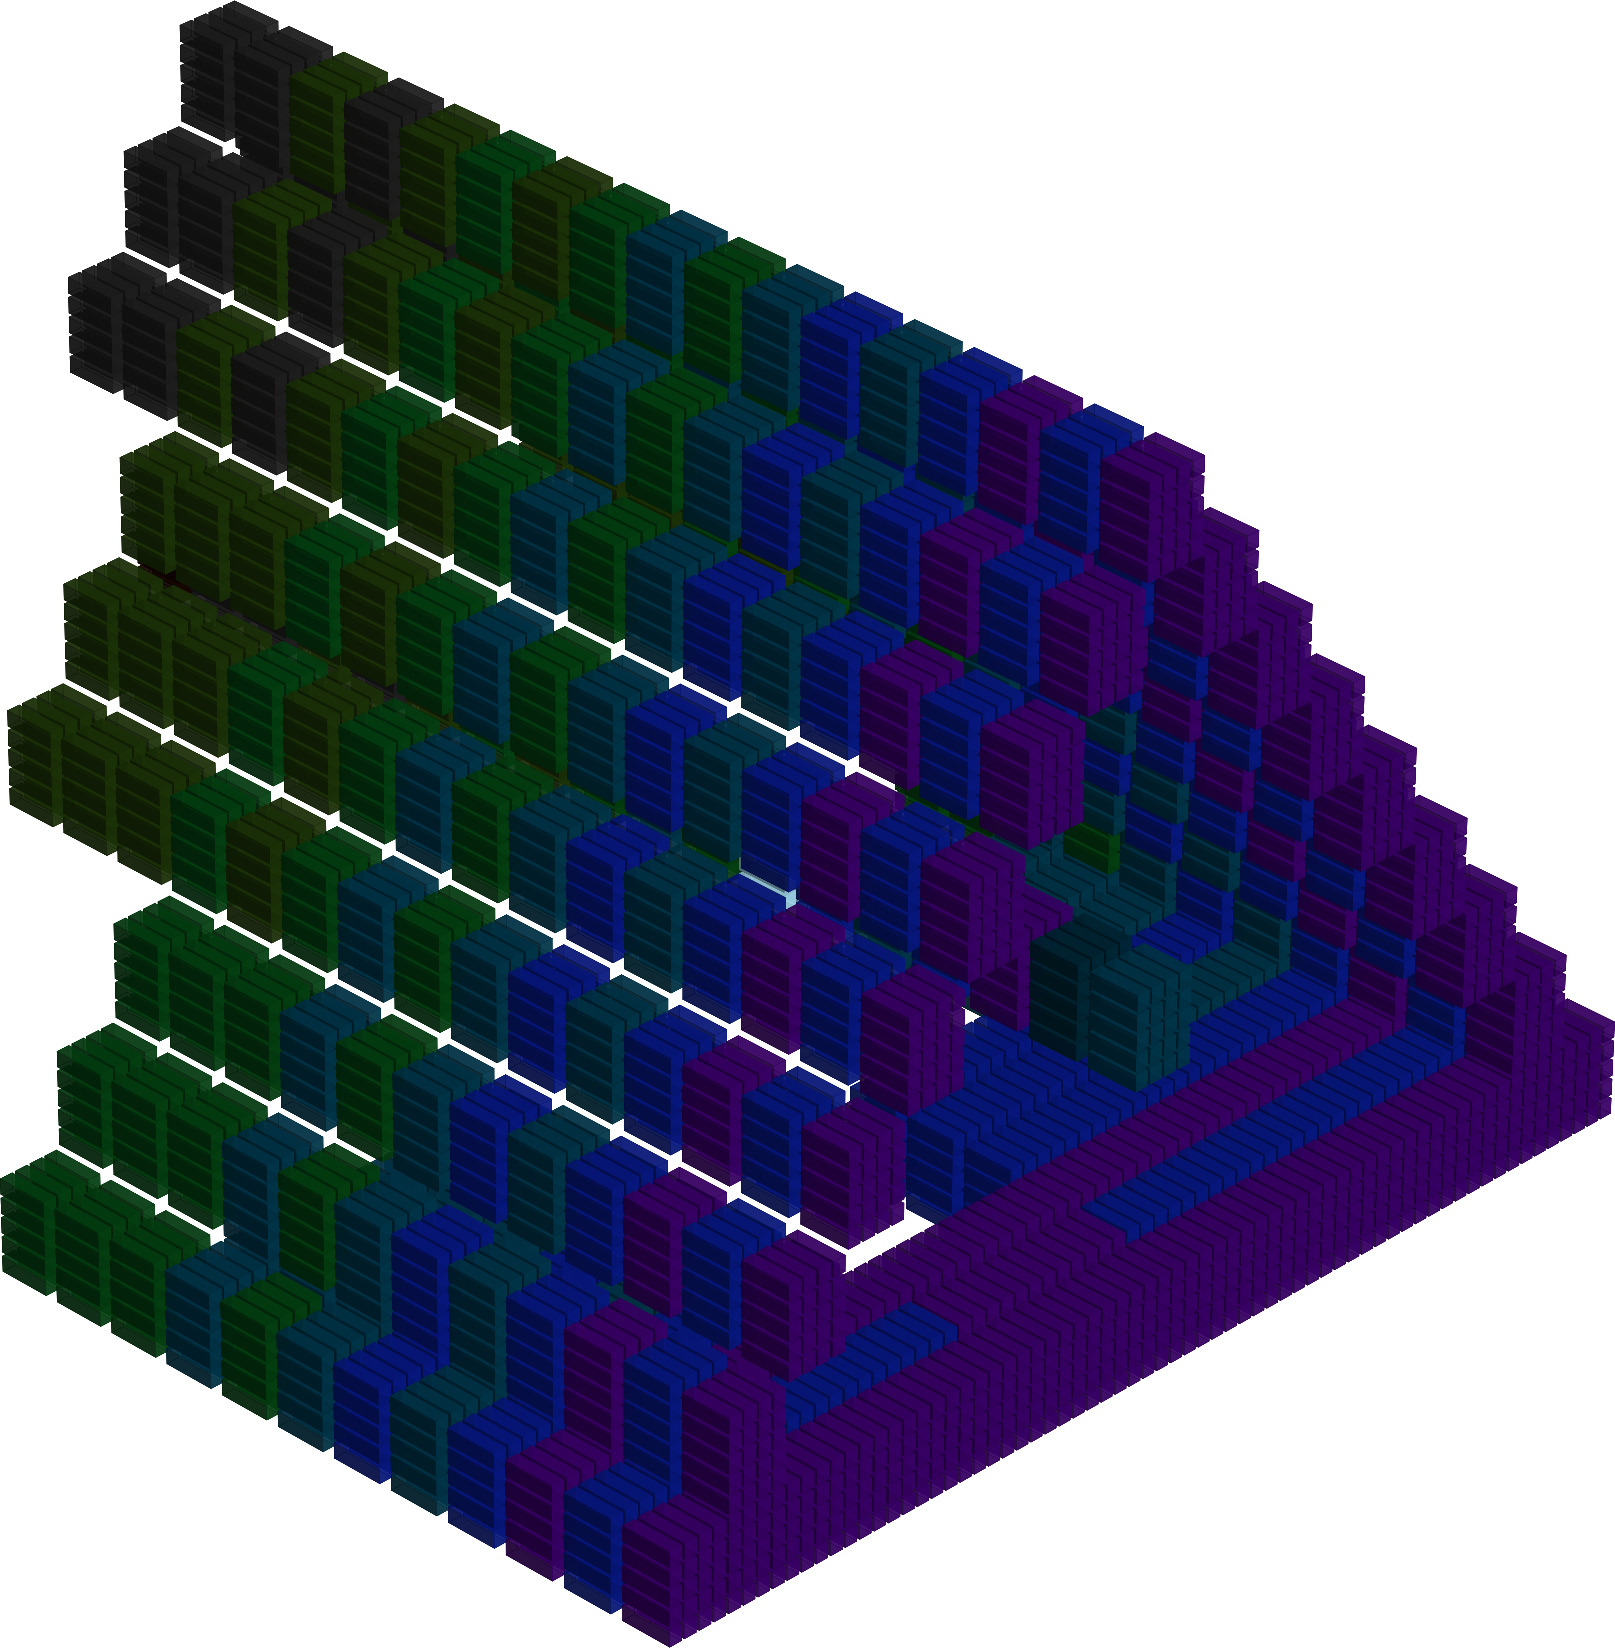
\includegraphics[width=10cm]{src/colorspace_patterns/pattern21-45.png}%
    \end{adjustbox}
    \begin{adjustbox}{width=5cm,margin=0cm 0cm}
      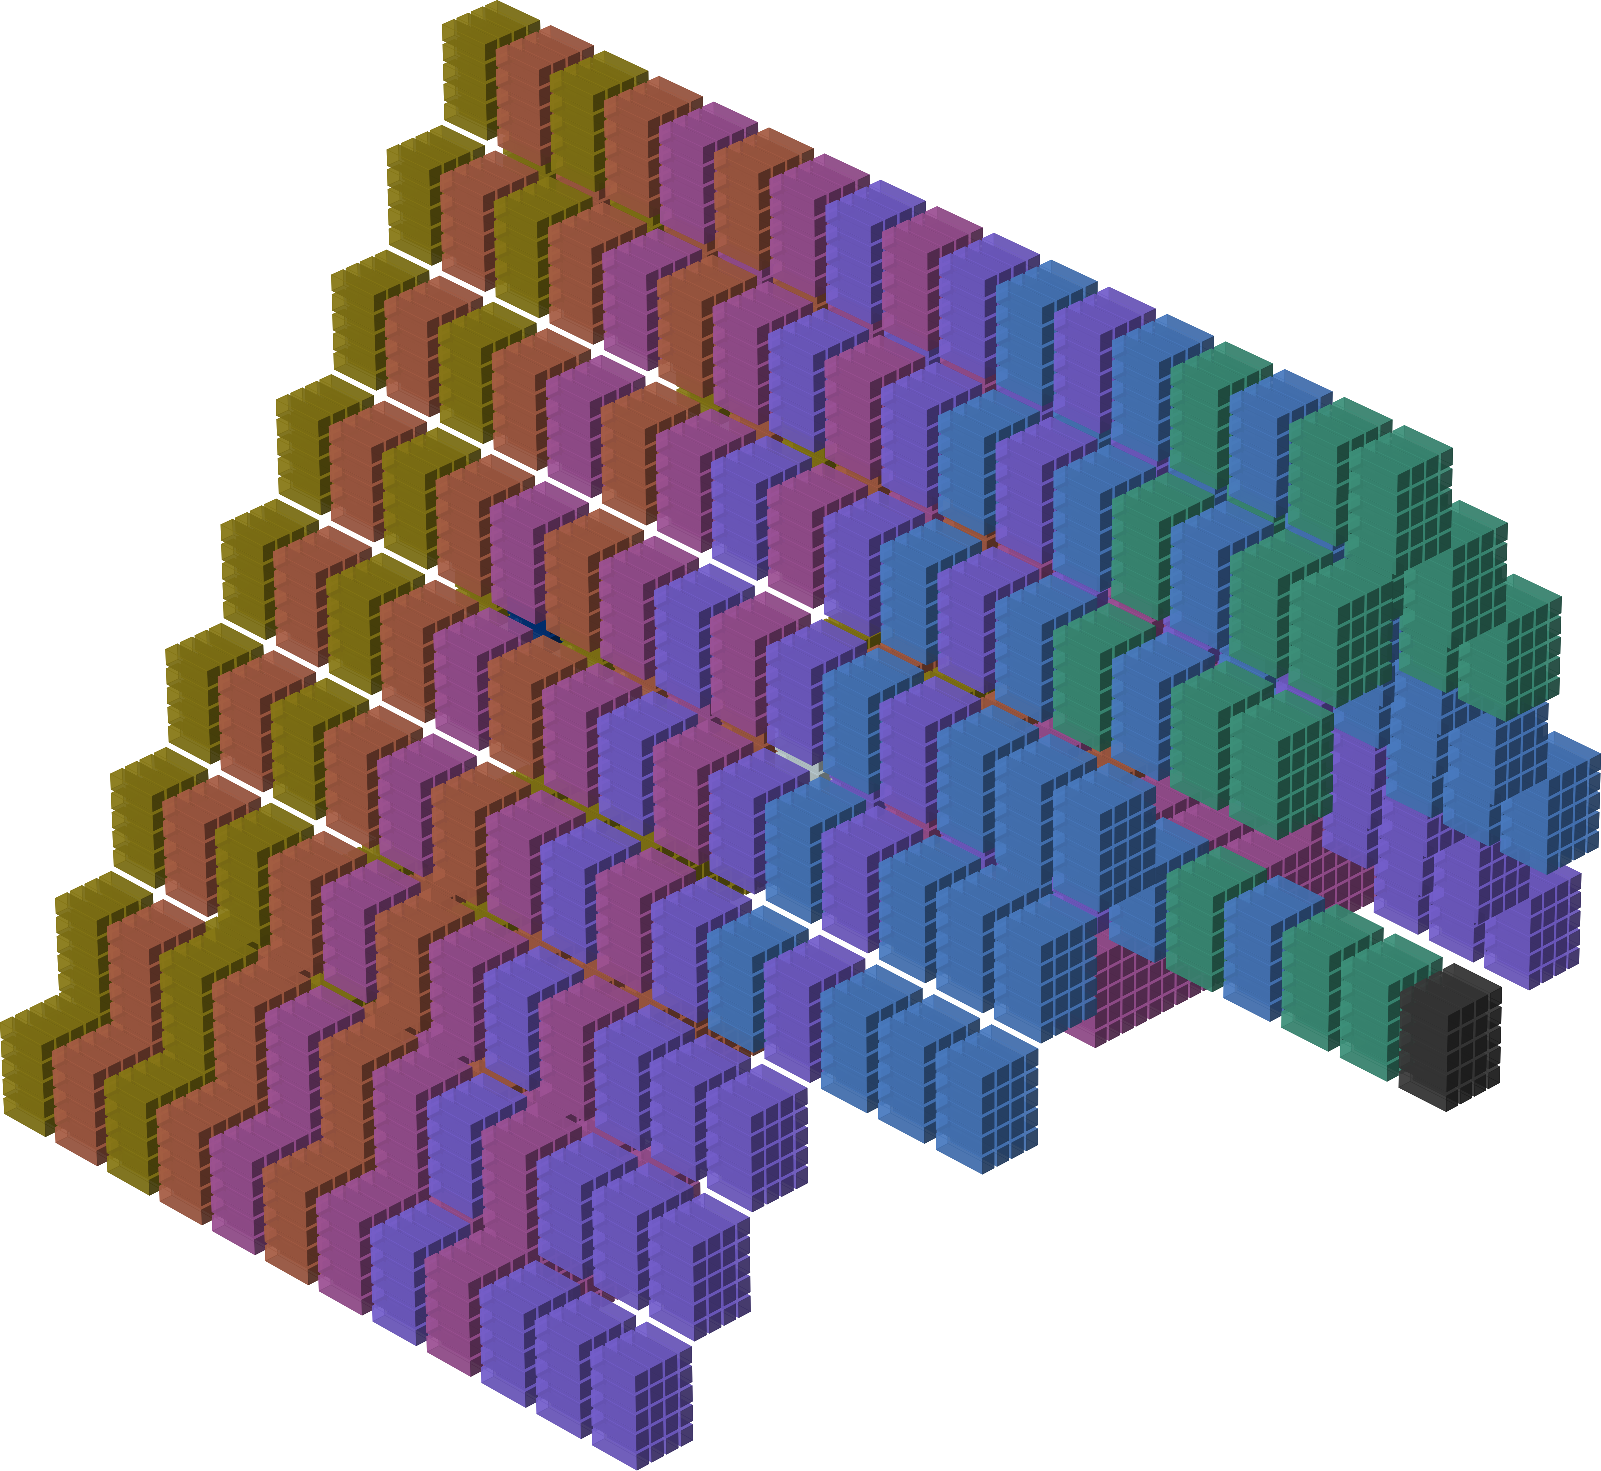
\includegraphics[width=10cm]{src/colorspace_patterns/pattern21-225.png}%
    \end{adjustbox}
\caption{'User LightForm 13'.}
\end{figure}
\end{minipage}
\begin{minipage}[b]{0.48\linewidth}
\begin{lrbox}{\mybox}%
\hspace{1cm}
\begin{lstlisting}[basicstyle=\ttfamily\tiny,escapechar=\%]
userLightform13XPosArray
        .BYTE $00,$FF,$01,$FE,$02,$55              ;         1        
        .BYTE $FD,$03,$FC,$04,$FB,$05,$55          ;        1 1       
        .BYTE $FA,$06,$F9,$07,$F8,$08,$55          ;       1   1      
        .BYTE $F9,$FA,$FB,$FC,$FD,$07,$06,$05,$55  ;      2     2     
        .BYTE $04,$03,$02,$01,$55                  ;     2       2    
        .BYTE $00,$FF,$FE,$55                      ;    2         2   
userLightform13YPosArray                           ;   3           3  
        .BYTE $FB,$FC,$FC,$FD,$FD,$55              ;  3             3 
        .BYTE $FE,$FE,$FF,$FF,$00,$00,$55          ; 34444466655554443
        .BYTE $01,$01,$02,$02,$03,$03,$55
        .BYTE $03,$03,$03,$03,$03,$03,$03,$03,$55
        .BYTE $03,$03,$03,$03,$55
        .BYTE $03,$03,$03,$55
\end{lstlisting}
\end{lrbox}%
\scalebox{0.8}{\usebox{\mybox}}
\subfile{colorspace_patterns/tables/pattern21.tex}
\end{minipage}
%
%
\begin{minipage}[b]{0.48\linewidth}
\vspace{0.5cm}
\begin{figure}[H]
    \centering
    \begin{adjustbox}{width=4cm,margin=0cm 0cm}
      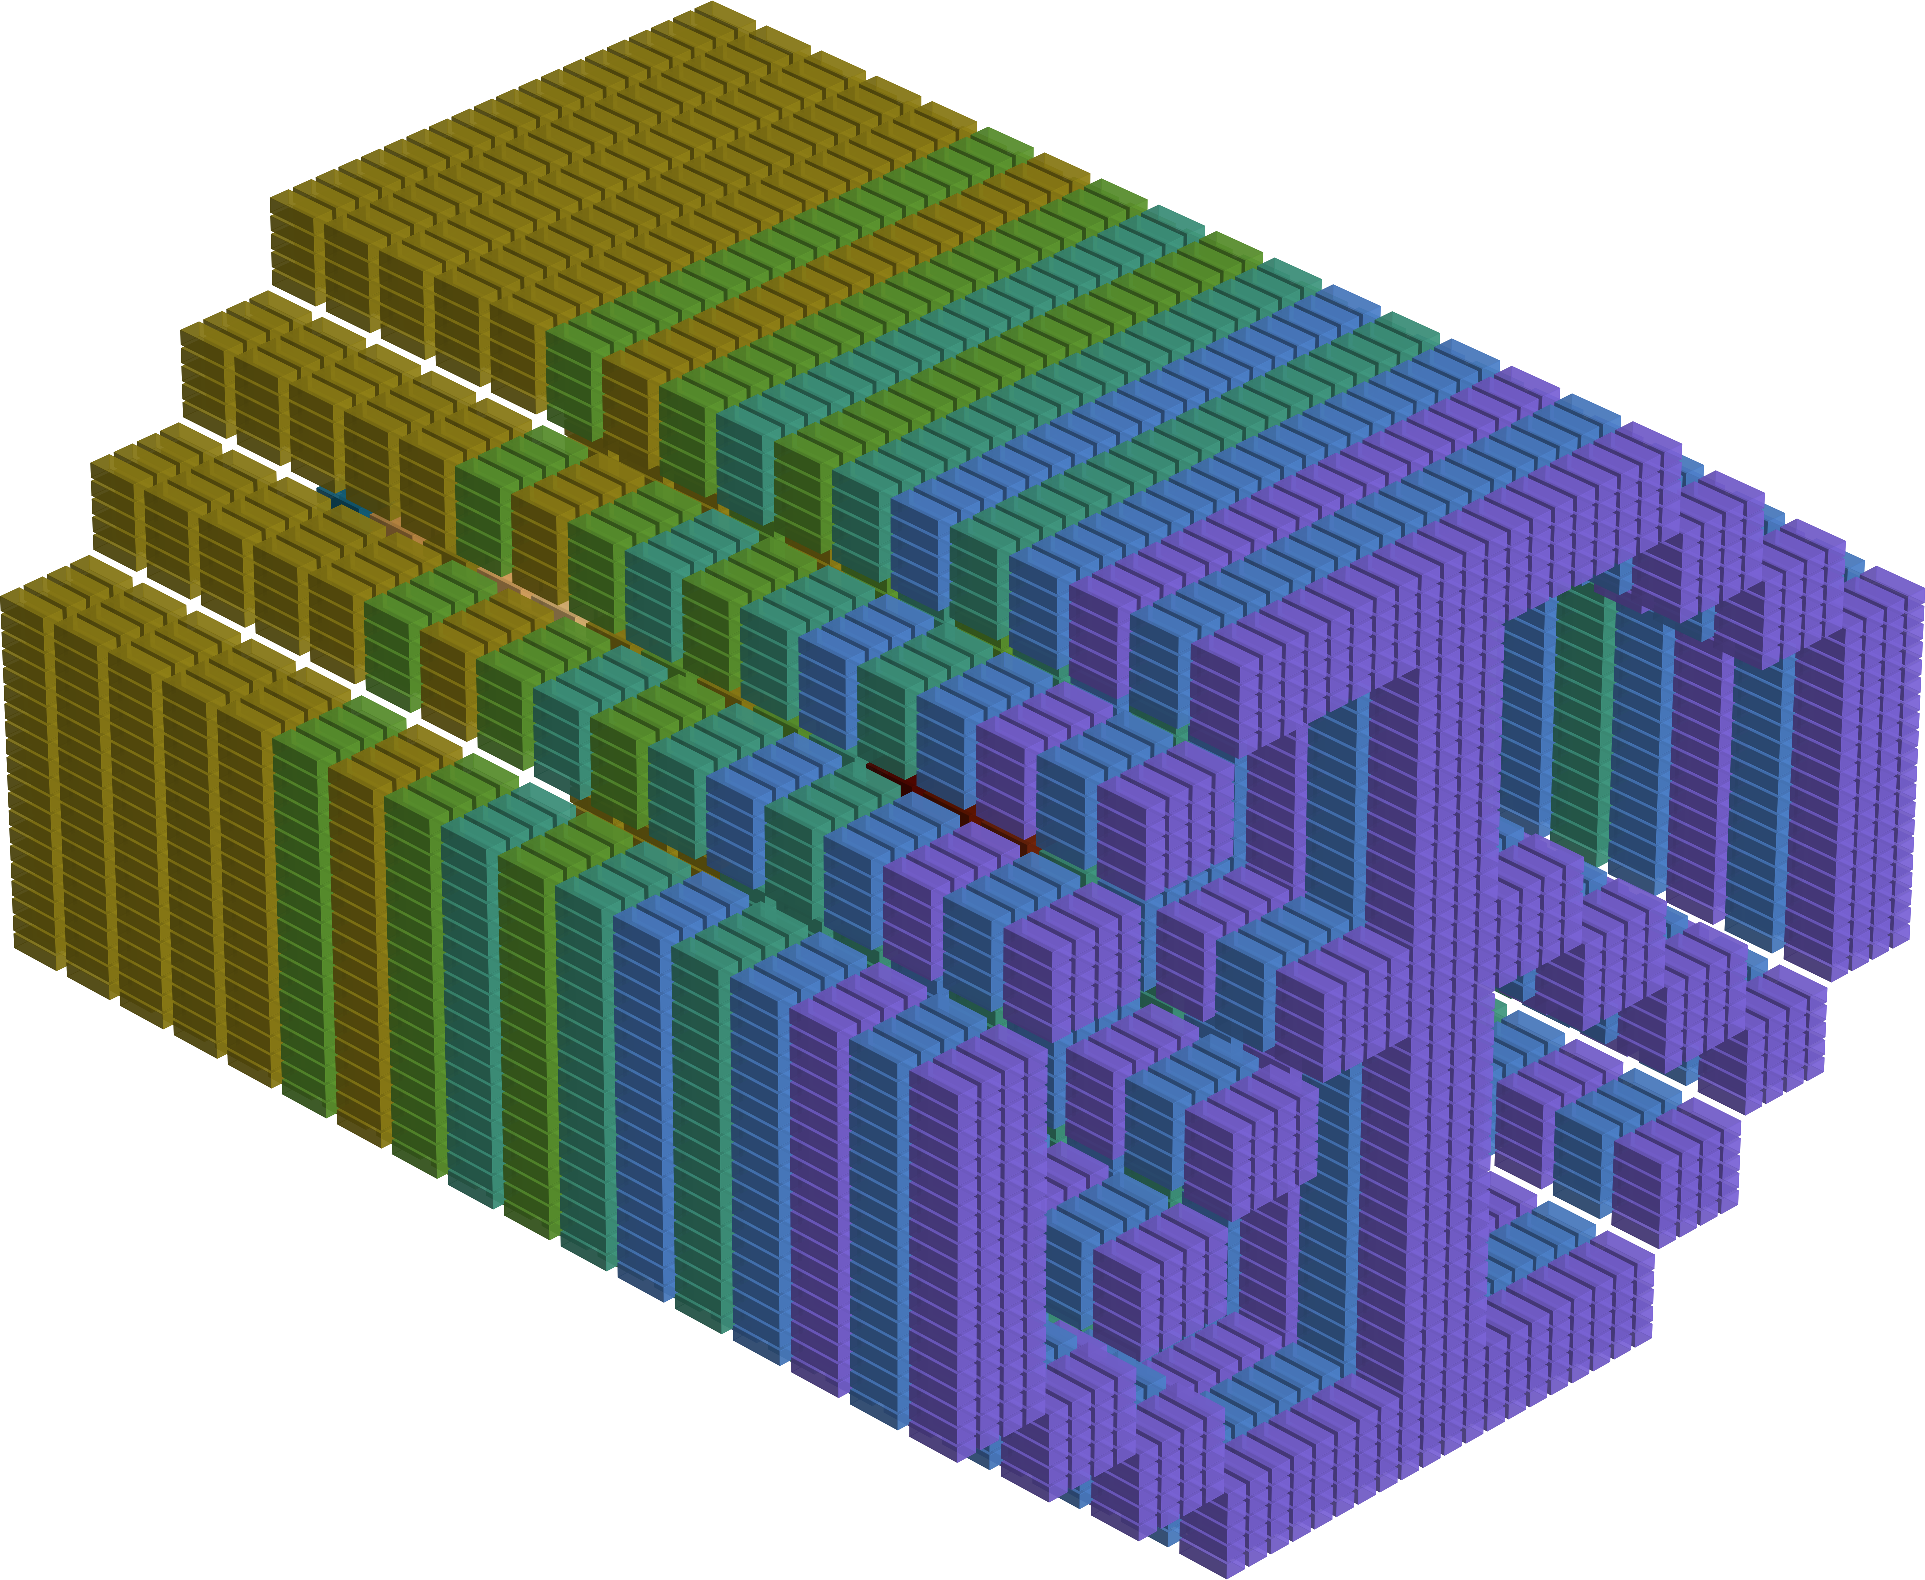
\includegraphics[width=10cm]{src/colorspace_patterns/pattern22-45.png}%
    \end{adjustbox}
    \begin{adjustbox}{width=4cm,margin=0cm 0cm}
      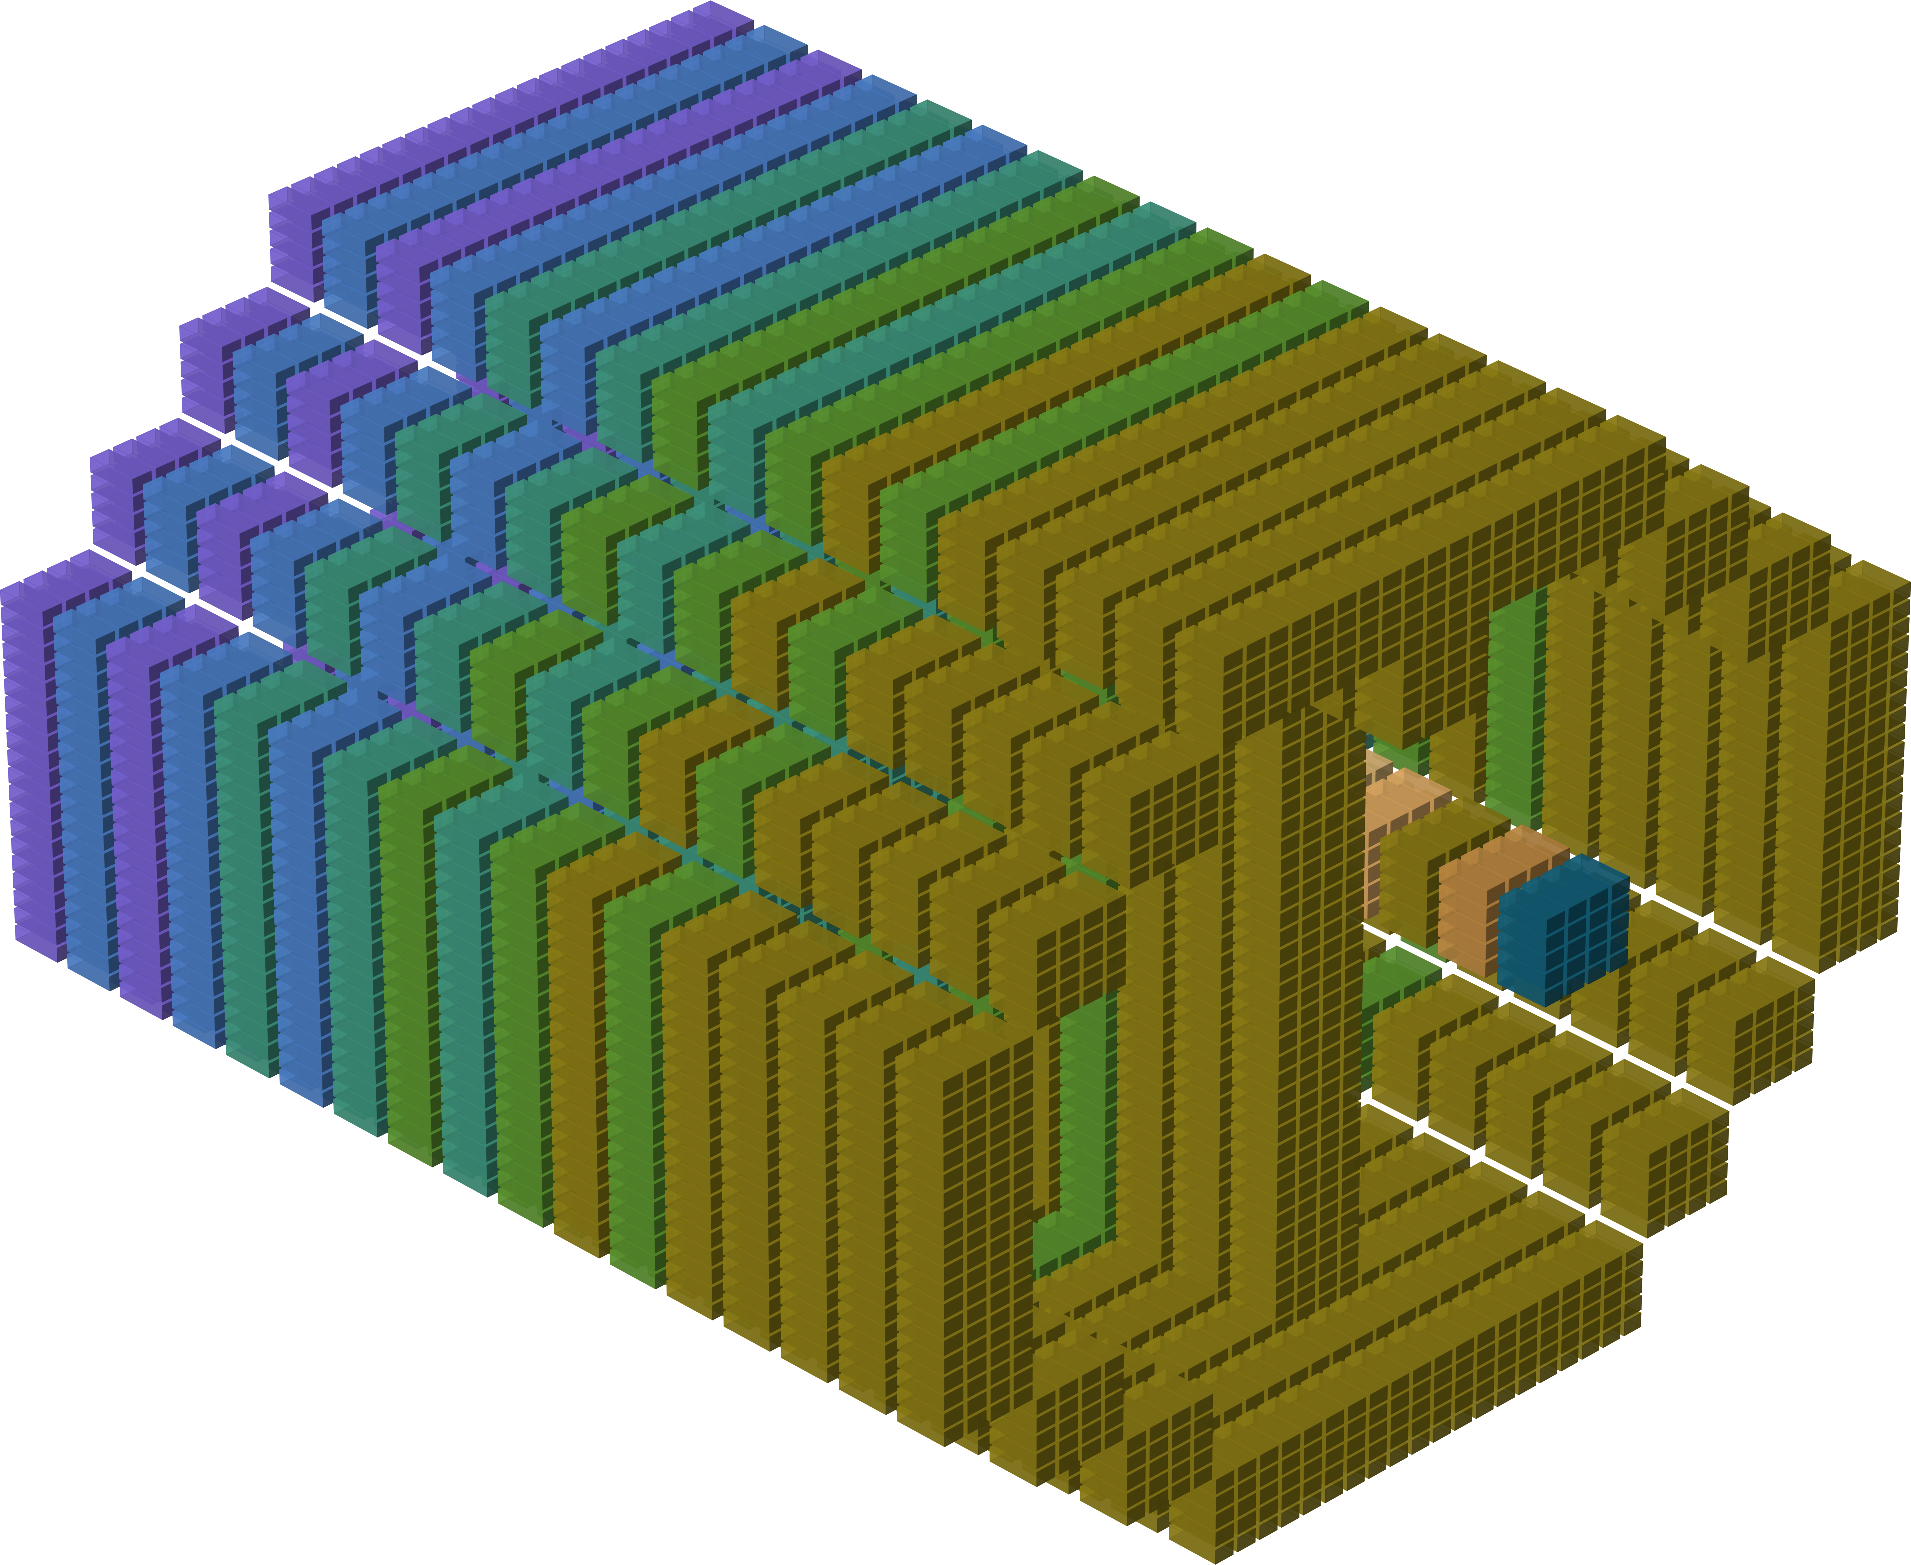
\includegraphics[width=10cm]{src/colorspace_patterns/pattern22-225.png}%
    \end{adjustbox}
\caption{'User LightForm 14'.}
\end{figure}
\end{minipage}
\begin{minipage}[b]{0.68\linewidth}
\vspace{0.5cm}
\begin{lrbox}{\mybox}%
\begin{lstlisting}[basicstyle=\ttfamily\tiny,escapechar=\%]
userLightform14XPosArray
  .BYTE $FC,$FC,$FC,$FD,$FE,$FF,$00,$01,$02,$FC,$FD,$FE,$FF,$00     ;    11111   
  .BYTE $01,$03,$03,$02,$04,$05,$06,$06,$06,$06,$05,$04,$01,$55     ;   1  1  1  
  .BYTE $01,$01,$01,$01,$01,$01,$01,$55                             ;  1   2   1 
  .BYTE $55                                                         ; 1    2    1
  .BYTE $FF,$FE,$02,$03,$04,$55                                     ; 1    24   1
userLightform14YPosArray                                            ; 1  4 2 4  1
  .BYTE $00,$01,$02,$03,$04,$05,$05,$05,$05,$FF,$FE,$FD,$FC,$FC     ; 1 4  2  4 1
  .BYTE $FC,$FC,$05,$FC,$FD,$FE,$FF,$00,$01,$02,$03,$04,$FD,$FE     ;  1   2   1 
  .BYTE $FE,$FF,$00,$01,$02,$03,$04,$55                             ;   1  2  1  
  .BYTE $55                                                         ;    11111   
  .BYTE $01,$02,$00,$01,$02,$55
\end{lstlisting}
\end{lrbox}%
\scalebox{0.8}{\usebox{\mybox}}
\subfile{colorspace_patterns/tables/pattern22.tex}
\end{minipage}
%
%
\begin{minipage}[b]{0.48\linewidth}
\begin{figure}[H]
    \centering
    \begin{adjustbox}{width=5cm,margin=0cm 0cm}
      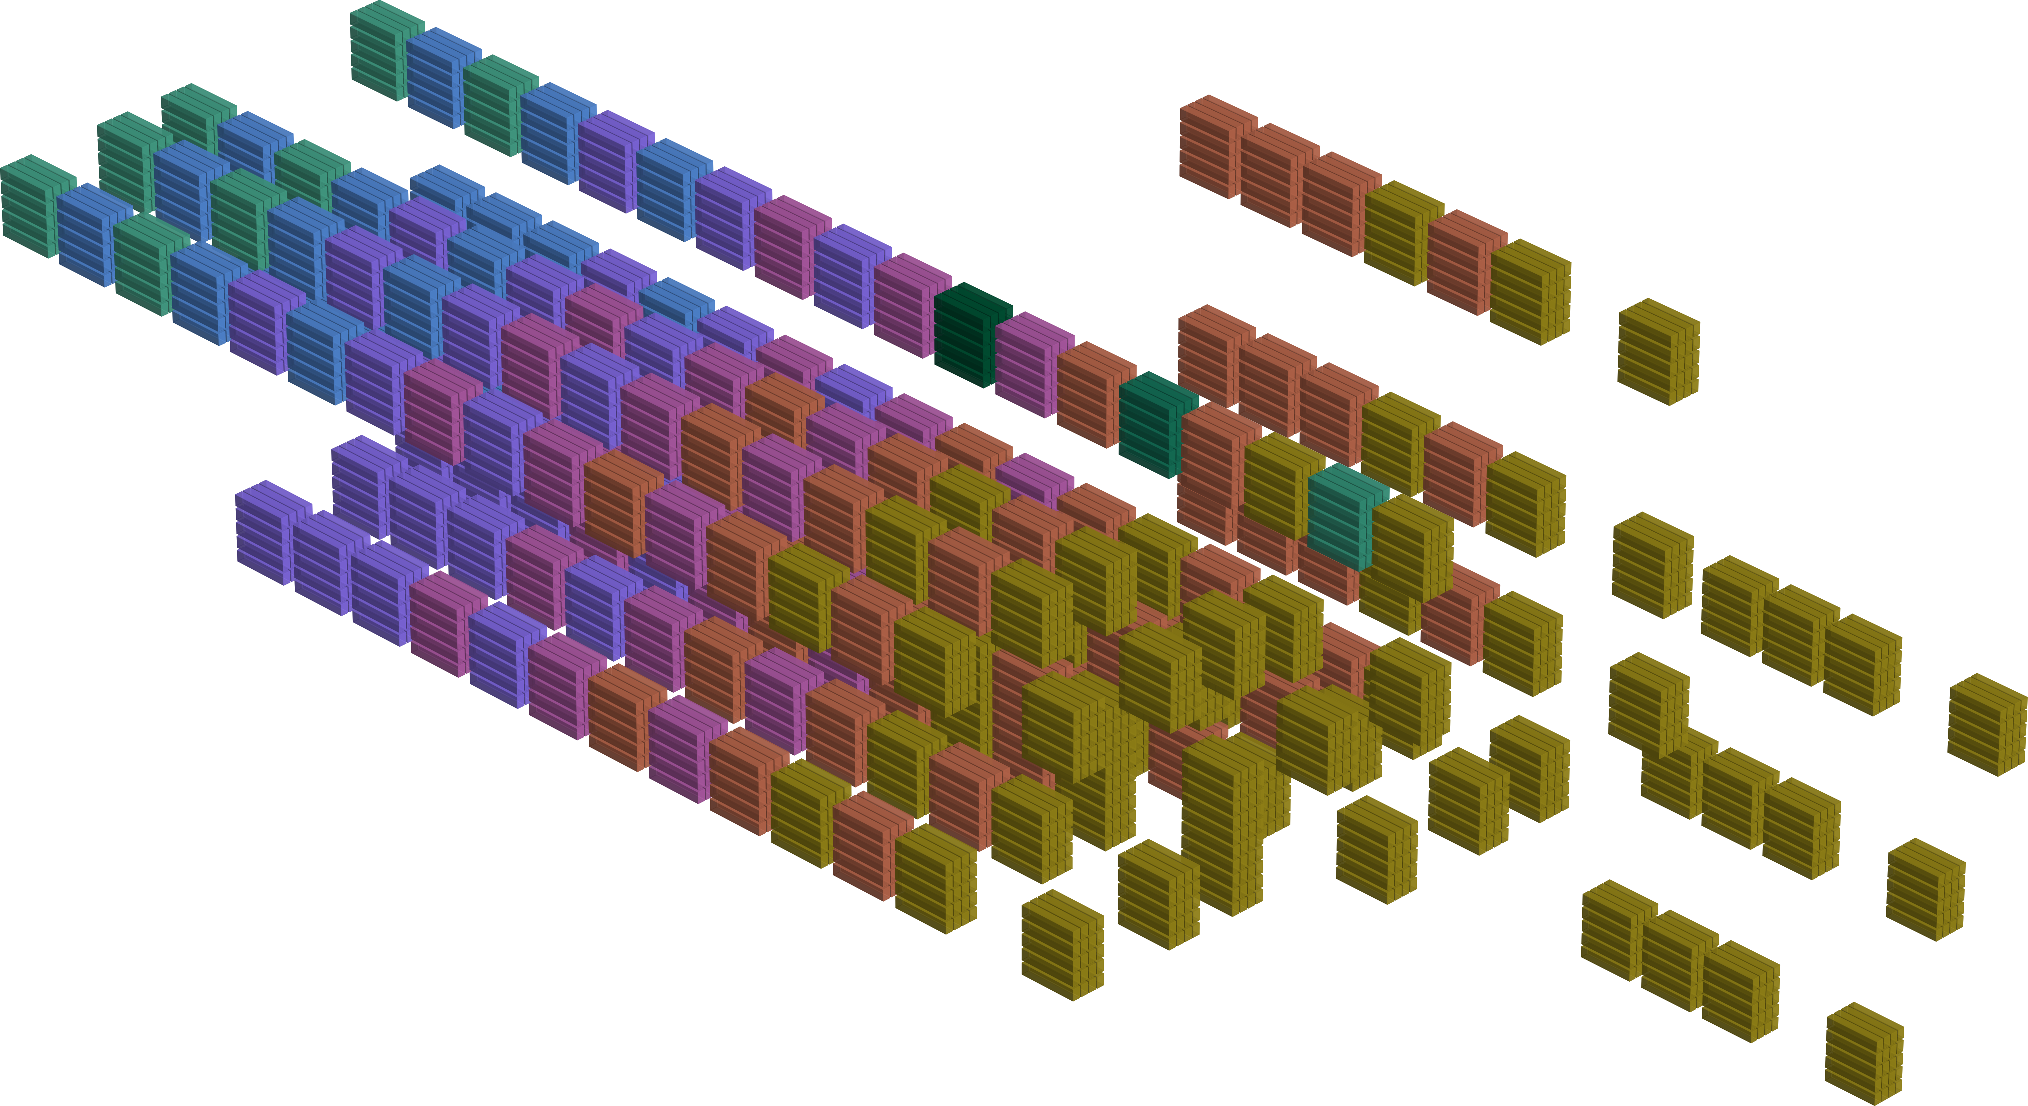
\includegraphics[width=10cm]{src/colorspace_patterns/pattern23-45.png}%
    \end{adjustbox}
    \begin{adjustbox}{width=5cm,margin=0cm 0cm}
      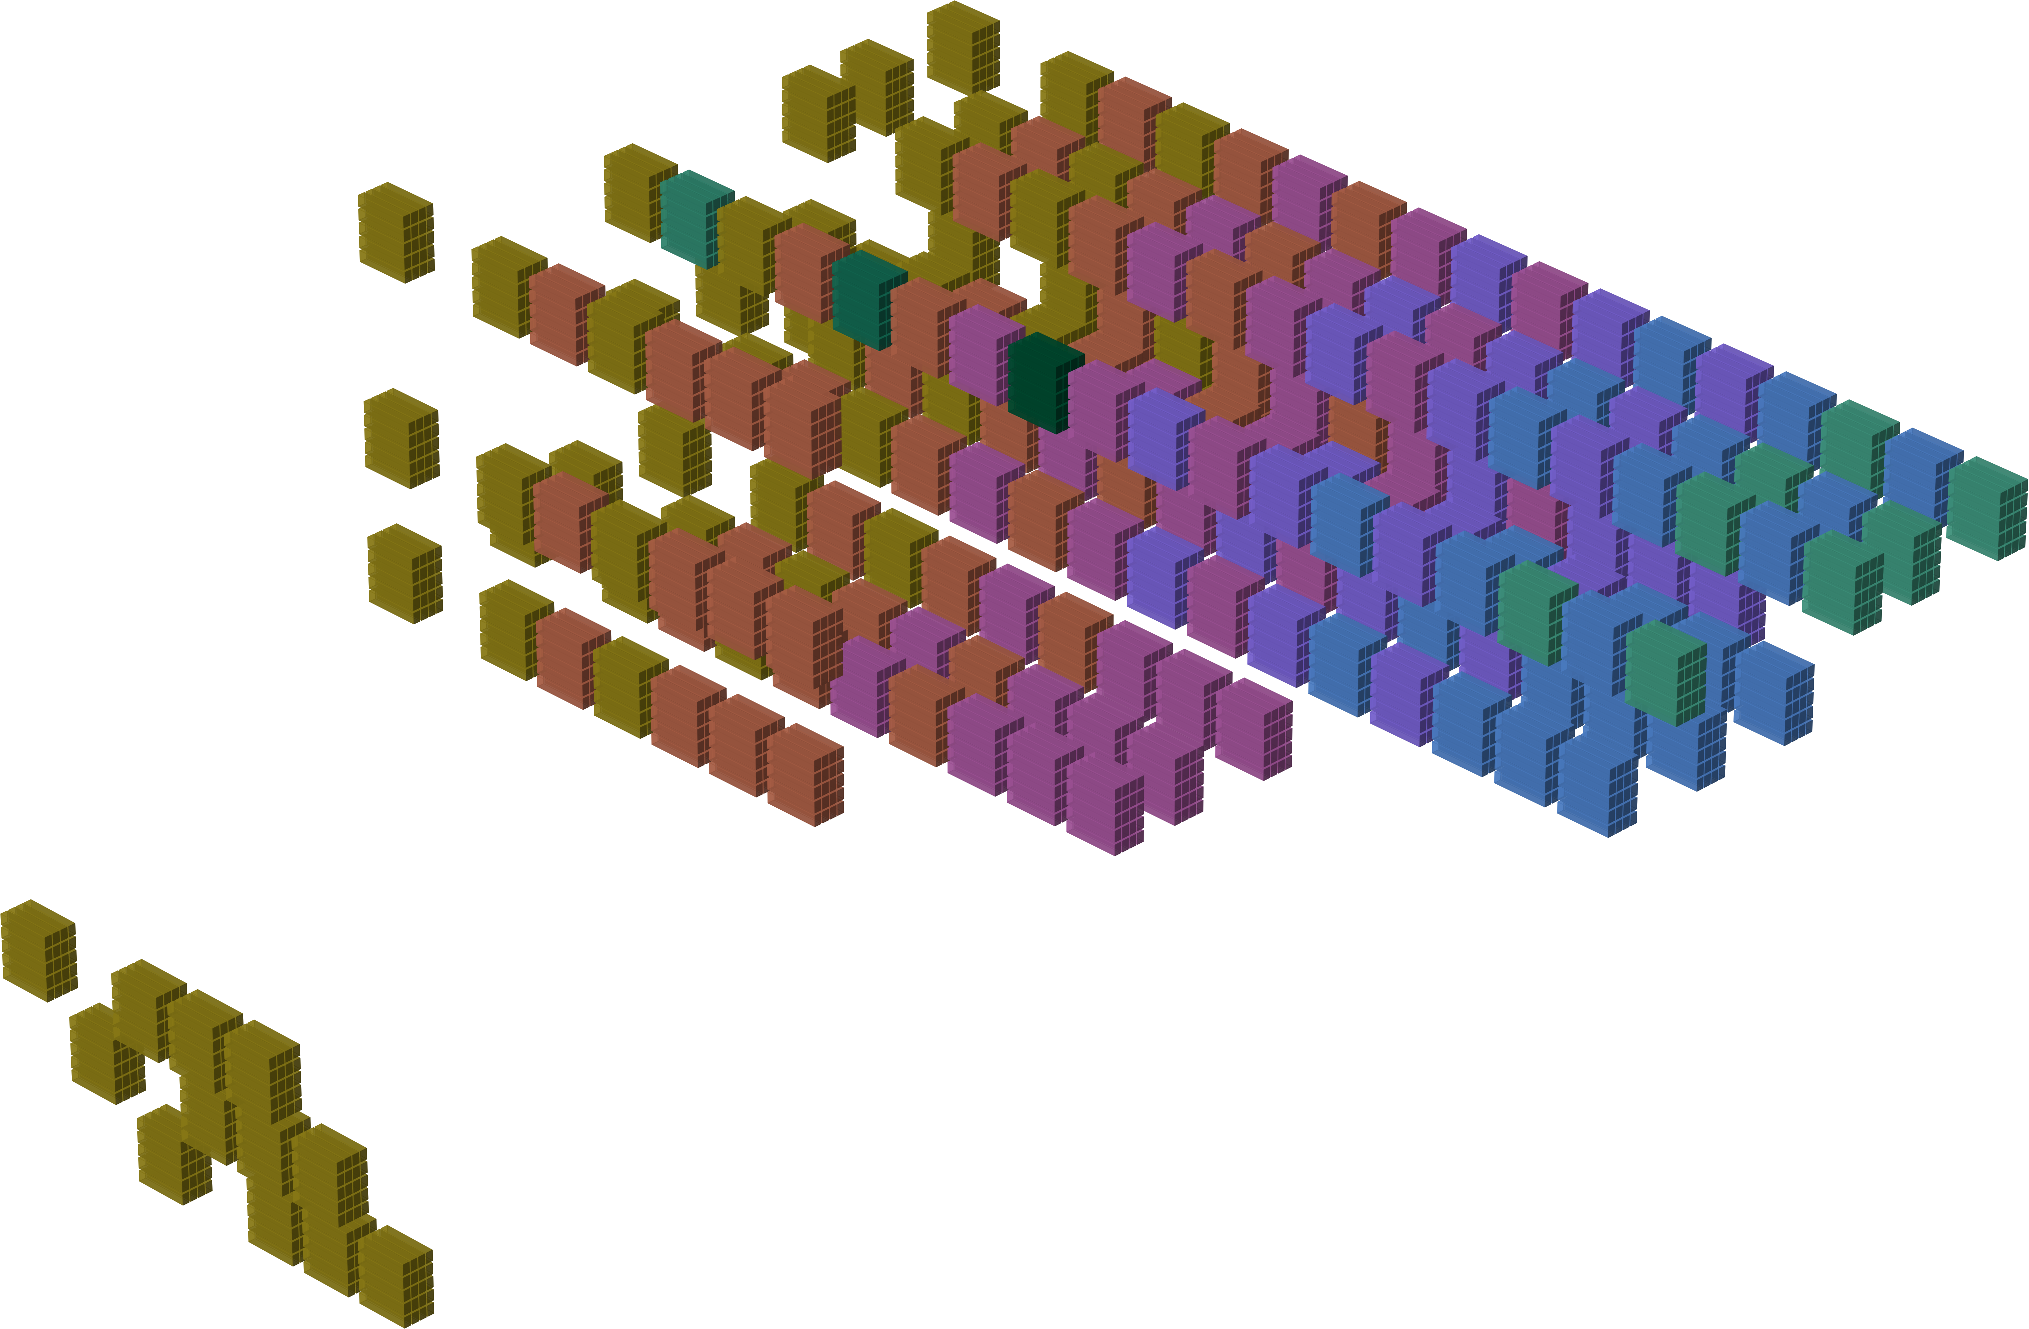
\includegraphics[width=10cm]{src/colorspace_patterns/pattern23-225.png}%
    \end{adjustbox}
\caption{'User LightForm 15'.}
\end{figure}
\end{minipage}
\begin{minipage}[b]{0.48\linewidth}
\begin{lrbox}{\mybox}%
\hspace{1cm}
\begin{lstlisting}[basicstyle=\ttfamily\tiny,escapechar=\%]
userLightform15XPosArray
.BYTE $F5,$F8,$FA,$55 ;                    5            
.BYTE $FA,$FD,$00,$55 ; 1  1 1                          
.BYTE $F5,$F8,$FA,$55 ;                                 
.BYTE $FF,$02,$04,$55 ;      2  2  2       5            
.BYTE $08,$08,$08,$55 ; 3  3 3                          
.BYTE $10,$12,$14,$55 ;           4  4 4   5            
userLightform15YPosArray
.BYTE $00,$00,$00,$55 ;                                 
.BYTE $02,$02,$02,$55 ;                                6
.BYTE $03,$03,$03,$55 ;                                 
.BYTE $04,$04,$04,$55 ;                              6  
.BYTE $FF,$02,$04,$55 ;                                 
.BYTE $0B,$09,$07,$55 ;                            6    
\end{lstlisting}
\end{lrbox}%
\scalebox{0.8}{\usebox{\mybox}}
\subfile{colorspace_patterns/tables/pattern23.tex}
\end{minipage}
%
